\documentclass[fleqn,usenatbib,useAMS]{mnras}
\usepackage{amsmath,amssymb}
\usepackage{xspace}
% \newcommand{\vdag}{(v)^\dagger}
% \newcommand\aastex{AAS\TeX}
% \newcommand\latex{La\TeX}
\usepackage{graphicx}
\usepackage{orcidlink}
\usepackage{comment}

% aliases for the DC1 PZ paper
\defcitealias{Schmidt20}{Schmidt \& Malz, et al.}
\newcommand{\citeDCp}{(\citetalias{Schmidt20} \citeyear{Schmidt20})\xspace}
\newcommand{\citeDCt}{\citetalias{Schmidt20} (\citeyear{Schmidt20})\xspace}
\newcommand{\citeDCa}{\citetalias{Schmidt20} \citeyear{Schmidt20}\xspace}

\newcommand{\PersonalTag}[3]{{\color{#2}{$^{#1}$ [#3}]}}
%\newcommand{\PersonalTag}[3]{}
\newcommand{\aim}[1]{\PersonalTag{Alex}{violet}{#1}}
\newcommand{\alice}[1]{\PersonalTag{Alice}{olive}{#1}}
\newcommand{\rachel}[1]{\PersonalTag{Rachel}{orange}{#1}}
\newcommand{\tianqing}[1]{\PersonalTag{Tianqing}{blue}{#1}}
\newcommand{\refresponse}[1]{{\color{black}{#1}}}
\newcommand{\revone}[2]{{\color{black}{#2}}}
\newcommand{\refresponsetwo}[1]{{\color{black}{#1}}}
\newcommand{\cwr}[1]{{\color{black}{#1}}}


% make a macro for yourself for making placeholder-y notes!
% color choices: black, blue, brown, cyan, darkgray, gray, green, lightgray, lime, magenta, olive, orange, pink, purple, red, teal, violet, white, yellow

\newcommand{\code}[1]{\texttt{#1}\xspace}
\newcommand{\cmnn}{\code{CMNN}}
\newcommand{\fzb}{\code{FlexZBoost}}
\newcommand{\gpz}{\code{GPz}}
\newcommand{\pzflow}{\code{PzFlow}}
\newcommand{\trainz}{\code{TrainZ}}
\newcommand{\rail}{\code{RAIL}}

\title[Diagnosing Spec-$z$ Imperfection on Photo-$z$]{Diagnosing the Effects of \cwr{Spectroscopic Training Set Imperfection} on Photometric Redshift Performance}

\author[]{%
Alice~Crafford\orcidlink{0009-0006-4576-2588},$^{1}$
Alex~I.~Malz\orcidlink{0000-0002-8676-1622},$^{2,1}$
Tianqing~Zhang\orcidlink{0000-0002-5596-198X},$^{1,3}$
Rachel~Mandelbaum\orcidlink{0000-0003-2271-1527},$^{1}$\thanks{E-mail: rmandelb@andrew.cmu.edu}
Olivia~Lynn\orcidlink{0000-0001-5028-146X},$^{1}$ \newauthor
Federico~Berlfein\orcidlink{0009-0004-4113-9938},$^{1}$
Johann~Cohen-Tanugi\orcidlink{0000-0001-9022-4232},$^{4}$
John~Franklin~Crenshaw\orcidlink{0000-0002-2495-3514},$^{5,6,7}$
Qianjun~Hang,$^{8}$\newauthor
Irene~Moskowitz\orcidlink{0000-0002-2206-8589},$^{9}$
Drew~Oldag\orcidlink{0000-0001-6984-8411},$^{10}$
Samuel~J.~Schmidt\orcidlink{0000-0002-5091-0470},$^{11}$
Ziang~Yan,$^{12,13}$\newauthor
and the LSST Dark Energy Science Collaboration
\\
$^{1}$McWilliams Center for Cosmology and Astrophysics, Department of Physics, Carnegie Mellon University, Pittsburgh, PA, USA\\
$^{2}$Space Telescope Science Institute, Baltimore, MD, USA\\
$^{3}$Department of Physics and Astronomy and PITT PACC, University of Pittsburgh, Pittsburgh, PA 15260, USA\\
$^{4}$Laboratoire de Physique de Clermont Auvergne, Universit\'e Clermont Auvergne and CNRS, Clermont-Ferrand, France\\
$^{5}$Kavli Institute for Particle Astrophysics and Cosmology, Stanford University, Stanford, CA, USA\\
$^{6}$Department of Physics, Stanford University, Stanford, CA 94305, USA\\
$^{7}$SLAC National Accelerator Laboratory, 2575 Sand Hill Road, Menlo Park, CA 94025, USA\\
$^{8}$Department of Physics \& Astronomy, University College London, Gower Street, London WC1E 6BT, UK\\
$^{9}$Department of Physics and Astronomy, Rutgers, The State University of New Jersey, Piscataway, NJ 08854, USA\\
$^{10}$DIRAC Institute, Department of Astronomy, University of Washington, Seattle, WA 98195, USA\\
$^{11}$Department of Physics, University of California, One Shields Avenue, Davis, CA 95616, USA\\
$^{12}$Faculty of Physics and Astronomy, Astronomical Institute (AIRUB), Ruhr University Bochum, German Centre for Cosmological\\Lensing, 44780 Bochum, Germany\\
$^{13}$Graduate School of Science, Nagoya University, Furocho, Chikusa-ku, Nagoya, Aichi 464-8602, Japan
}



\begin{document}

\maketitle


% \footnote{Released on March, 1st, 2021}}

% \author[0009-0006-4576-2588]{Alice Crafford}
% \affiliation{McWilliams Center for Cosmology and Astrophysics, Department of Physics, Carnegie Mellon University, Pittsburgh, PA, USA}

% \author[0000-0002-8676-1622]{Alex I. Malz}
% \affiliation{Space Telescope Science Institute, Baltimore, MD, USA}
% \affiliation{McWilliams Center for Cosmology and Astrophysics, Department of Physics, Carnegie Mellon University, Pittsburgh, PA, USA}

% \author[0000-0002-5596-198X]{Tianqing Zhang}
% \affiliation{McWilliams Center for Cosmology and Astrophysics, Department of Physics, Carnegie Mellon University, Pittsburgh, PA, USA}
% \affiliation{Department of Physics and Astronomy and PITT PACC, University of Pittsburgh, Pittsburgh, PA 15260, USA}

% \author[0000-0003-2271-1527]{Rachel Mandelbaum}
% \affiliation{McWilliams Center for Cosmology and Astrophysics, Department of Physics, Carnegie Mellon University, Pittsburgh, PA, USA}

% \author[0000-0001-5028-146X]{Olivia Lynn}
% \affiliation{McWilliams Center for Cosmology and Astrophysics, Department of Physics, Carnegie Mellon University, Pittsburgh, PA, USA}

% \author[0009-0004-4113-9938]{Federico Berlfein}
% \affiliation{McWilliams Center for Cosmology and Astrophysics, Department of Physics, Carnegie Mellon University, Pittsburgh, PA, USA}

% \author[0000-0001-9022-4232]{Johann Cohen-Tanugi}
% \affiliation{Laboratoire de Physique de Clermont Auvergne, universit\'e de Clermont Auvergne and CNRS, France}

% \author[0000-0002-2495-3514]{John Franklin Crenshaw}
% \affiliation{Kavli Institute of Particle Astrophysics and Cosmology}
% \affiliation{Department of Physics, Stanford University, Stanford, CA, USA 94305-4085}
% \affiliation{SLAC National Accelerator Laboratory 2575 Sand Hill Road Menlo Park, California 94025, USA}

% \author{Qianjun Hang}
% \affiliation{Department of Physics \& Astronomy, University College London, Gower Street, London WC1E 6BT, UK}

% \author[0000-0002-2206-8589]{Irene Moskowitz}
% \affiliation{Department of Physics and Astronomy, Rutgers, The State University of New Jersey, Piscataway, NJ 08854, USA}

% \author[0000-0001-6984-8411]{Drew Oldag}
% \affiliation{DIRAC Institute, University of Washington, Seattle, WA 98195, USA}

% \author[0000-0002-5091-0470]{Samuel J. Schmidt}
% \affiliation{Department of Physics, University of California, One Shields Avenue, Davis, CA 95616, USA}

% \author{Ziang Yan}
% \affiliation{Ruhr University Bochum, Faculty of Physics and Astronomy, Astronomical Institute (AIRUB), German Centre for Cosmological Lensing, 44780 Bochum, Germany}
% \affiliation{Graduate School of Science, Nagoya University, Furocho, Chikusa-ku, Nagoya, Aichi, 464-8602, Japan}

% \author{the LSST Dark Energy Science Collaboration}
%% Withdrew authorship request at her own choice for personal reasons, emailed Rachel
%\author{Julia Gschwend}
%\affiliation{Laboratorio Interinstitucional de e-Astronomia (LIneA), Rua General Jose Cristino, 77, Rio de Janeiro, Brazil}

% \author{August Muench}
% \affiliation{American Astronomical Society \\
% 1667 K Street NW, Suite 800 \\
% Washington, DC 20006, USA}

% \collaboration{20}{(AAS Journals Data Editors)}

% \author{F.X Timmes}
% \affiliation{Arizona State University}
% \affiliation{AAS Journals Associate Editor-in-Chief}

% \author{Amy Hendrickson}
% \altaffiliation{AASTeX v6+ programmer}
% \affiliation{TeXnology Inc.}

% \author{Julie Steffen}
% \affiliation{AAS Director of Publishing}
% \affiliation{American Astronomical Society \\
% 1667 K Street NW, Suite 800 \\
% Washington, DC 20006, USA}


 
\begin{abstract}%
Most LSST extragalactic science will rely on photometric redshifts (photo-$z$) to extract distance information for the galaxies. 
However, an incomplete or non-representative training set can introduce bias into photo-$z$ estimation. 
It is necessary to understand how various forms of training set imperfection, such as incompleteness and non-trivial spectroscopic target selection, affect photo-$z$ estimation algorithms, and to identify metrics best-suited to quantify the impact.
% with which we can most effectively identify these effects. 
This work aims to systematically study metrics for diagnosing how various photo-$z$ methods react to certain types of training set incompleteness and non-representativeness. 
We use methods available through the open-source Python library Redshift Assessment Infrastructure Layers (\texttt{RAIL}; \citealt{2025arXiv250502928T}) to systematically test the algorithms \texttt{CMNN}, \texttt{GPz}, \texttt{FlexZBoost}, and \texttt{PZFlow} on mock training data degraded in accordance with several existing spectroscopic sky surveys, as well as under conditions of inverse redshift incompleteness\refresponse{, which approximately mimics observed patterns of incompleteness at high redshift}. 
We employ the algorithm \texttt{TrainZ} as a control.
Finally, we quantify photo-$z$ algorithm performance using a variety of statistical metrics  implemented externally to RAIL. 
We determine that the Kullback-Liebler Divergence, Wasserstein Distance, and Probability Integral Transform are particularly informative metrics with which to assess the impact of training set imperfection on algorithmic performance. 
We also find that inverse redshift incompleteness effects alone lack the complexity to realistically represent anticipated training data. 
\end{abstract}

%\rachel{I suggest updating the title to `Diagnosing the Effects of Imperfect Spectroscopic Training Sets on Photometric Redshift Performance' to highlight the metrics and analysis methods rather than the specific failure modes for the estimators and simulation used in this work.}

\begin{keywords}
  galaxies: distances and redshifts -- methods: statistical
\end{keywords}

\section{Introduction} \label{sec:intro}
%\alice{We can write this at the end}

The Vera C.~Rubin Observatory Legacy Survey of Space and Time (LSST, \citealt{ivezic2019}) will collect the largest-ever imaging survey dataset in the next decade. LSST will detect and observe $\sim 10^{9}$ galaxies\revone{ in the universe}{}, which is transformative for many extragalactic science cases. 
Spectroscopic measurements will not be available for most galaxies in LSST due to its depth and sheer data volume; 
therefore, it will be necessary to estimate the redshift of the galaxies based on their photometry. 
Such techniques are referred to as photometric redshifts, or photo-$z$ \citep[for a review, see][]{2019NatAs...3..212S,2022ARA&A..60..363N}. 

Most \refresponse{data-driven photo-$z$ algorithms} require a training set (photometry cross-matched with precise redshift measurements from spectroscopic surveys). 
Because photo-$z$ point estimates are subject to nontrivial statistical and systematic uncertainties, redshifts are best characterized by posterior probability density functions (PDFs) that enable quantification of non-Gaussian error;
the designation of posterior conveys that data-driven algorithms typically estimate redshifts conditioned on photometric data rather than the probability of the observed photometry conditioned on redshift, which is only possible with a physical model.
\citeDCt explored the quality of photo-$z$ PDFs for different estimators under idealized conditions, i.e.~a perfectly representative and complete training set of generous size\revone{}{ yet nonetheless uncovered several major areas for improvement in the field of photo-$z$}. 

\revone{However}{Most obviously}, a realistic training set will likely never be a representative subsample as the faint galaxy samples used for cosmological measurements in LSST, due to different sensitivities of spectroscopic instruments along with the spectroscopic survey selection functions \citep{Stylianou22}, \refresponse{and the specific training set conditions to which various estimation algorithms are sensitive or performant is not yet adequately understood. } \cwr{The mismatch between the training set and the photometric sample to which the photometric redshift estimators are to be applied induces a statistical effect known as `covariate shift'.} 
This experiment picks up from \citeDCt by testing empirical estimators under realistically imperfect assumptions of training set size, completeness, and representativity \cwr{to assess their sensitivity to this covariate shift}.

\revone{}{However, the other findings of \citeDCt were more subtle.
First, the most commonly used metrics of photo-$z$ performance were shown to \refresponsetwo{have a failure mode wherein they responded favorably to a pathological approach to photo-$z$ that does not use the galaxy photometry.  Since the key factor} we wish to assess about a given estimator and prior information \refresponsetwo{is how well they extract redshift information from photometry, this finding highlighted} a need for exploration and vetting of potential performance metrics for the purpose of identifying promising estimators and characterizing their sensitivity to training set imperfection.
Second, the statistical metrics available for exploration depend on what truth information is accessible;
if true redshifts are known, they may be compared to photo-$z$ point estimates, but without true posterior PDFs, there are limited options for evaluating estimated posterior PDFs.}

\revone{}{This work is a follow-up to \citeDCt, but it is not a data challenge aiming to vet estimators against one another;
rather, we aim to inform the way in which such a vetting should be done in order to best select and optimize photo-$z$ algorithms.
To that end, our experiments focus on the metrics by which photo-$z$ estimation is assessed, rigorously testing those against one another in controlled experiments of training set imperfection on a non-exhaustive subset of estimators, considering the sensitivity of the metrics to the degree and type of imperfection in relation to the differences between algorithm types.
The metric(s) used to choose and tune algorithms for various science cases should reflect the inherent and thus anticipated worsening of redshift information recovery as data quality drops regardless of the choice of estimator\refresponsetwo{. I}t should be possible to interpret an estimator's favorable metric value in terms of some information-maximizing property of the \refresponsetwo{estimator} itself rather than a \refresponsetwo{failure of the metric to respond well to changes in the estimator's performance due to some quirk in how the metric was designed}.}

Our work uses the open-source Python package Redshift Assessment Infrastructure Layers (RAIL\revone{}{; \citealt{2025arXiv250502928T}})\revone{,  to facilitate}{ that was designed to enable the photo-$z$ community to address the concerns highlighted by \citeDCt by facilitating} data generation and large-volume analysis of photo-$z$ algorithms. 
RAIL provides a library of modules to generate mock photometric catalogs as training sets, a collection of data-driven and template-fitting algorithms to estimate photo-$z$ PDFs, and statistical metrics to evaluate the performance of individual runs. 
All RAIL functionality is written into stages, with the vision that users may connect different stages and turn them into an end-to-end data processing pipeline. 

One of the capabilities of RAIL is to generate a realistic photometric catalog through its ``creation'' modules. 
The creation modules have two main functionalities: (a) the engines emulate the photometry-redshift relation learned from sophisticated simulations, such as \citet{Korytov2019} and \citet{Troxel2023}; (b) the degraders add LSST-like noise and apply spectroscopic selections to the truth catalog to produce a realistic catalog for training and testing purposes. 
These functionalities enable the study of the training set incompleteness and non-representativity effects on the \refresponse{photo-$z$}, as its more extensive collection of tunable degradation stages allows us to approach the realistic complexity of the datasets that will be collected by LSST.  
RAIL \revone{is also}{also provides a shared API to access} a library of more than a dozen photo-$z$ estimation algorithms, including data-driven, template-fitting, and image-based algorithms. 
In this study, we apply five different photo-$z$ estimation algorithms implemented in RAIL on the degraded training set, to study their sensitivity to different types and levels of imperfection in the training set. 

In this study, we are interested in different statistical metrics that help quantify the imperfections in photo-$z$ due to imperfect training sets\revone{.  
We are particularly interested in}{, especially} the metrics that compare the estimated posterior PDF to the true posterior PDF of the galaxy, which is defined as the conditional probability \refresponsetwo{distribution} of the redshift given the photometry \revone{}{in the absence of bias due to an estimator or prior information;
this quantity was inherently unavailable in the study of \citeDCt but is accessible for photometry forward-modeled by RAIL's creation functionality and critical to evaluating estimators of photo-$z$ PDFs}.  
We apply seven such metrics to the estimated PDF to study their behavior\revone{.}{, aiming to determine whether they are suitable for assessing the sensitivity of estimators to imperfect prior information and for comparing estimators to one another.
A good metric should be sensitive to how well an estimator extracts redshift information from imperfect photometry under imperfect prior information, demonstrating sensitivity to when either of these inputs worsens, for any estimator;
if we can draw conclusions demonstrating that it holds for the choice of estimator, our findings can inform not only assessments of training set requirements but also optimization of the values of tuning parameters of an estimator and even the choice of estimator itself.}  
\refresponse{In all cases, we are quantifying the performance of individual galaxy photo-$z$ with basic statistical methods.  
This sets the stage for future studies that must also consider science-driven metrics and the performance for galaxy ensembles rather than individual photo-$z$.}

The paper is organized as follows. Section~\ref{sec:methodsdata} introduces the methodology, including the data generation, degradation, and photo-$z$ estimation methods.  It also describes the data used for training the truth catalog emulator.  Section~\ref{sec:metrics} describes the different statistical methods used to \refresponse{quantify} photo-$z$ quality, and provides some intuition regarding their interpretation.  Section~\ref{sec:results} describes the results of our experiments and our observation of how different patterns in training set degradation are reflected in different statistical metrics for each photo-$z$ algorithm. In Section~\ref{sec:conclusion}, we discuss our conclusions from these experiments, and their implications for the future.  


% The RAIL stage infrastructure was used in order to perform much of our experiment. 
% This comprehensive analysis was designed to use many combinations of training set degradation and estimation technique, in order to approximate realistic data complexities

% \aim{TODO for Alex: 
% Based on the rest of the paper, here are things to definitely be sure to address in the introduction beyond the basic background (or at least somewhere before the places where they come up):
% \begin{itemize}
%     % \item What is the significance of PDFs as opposed to point estimates?  (before \S~\ref{sec:estimators})
%     % \item Posterior vs. likelihood (before \S~\ref{sec:metrics})
%     % \item What is RAIL? What are stages? What is a degrader? (before \S~\ref{sec:overview})
% \end{itemize}
% }

\begin{figure*}
  \centering
  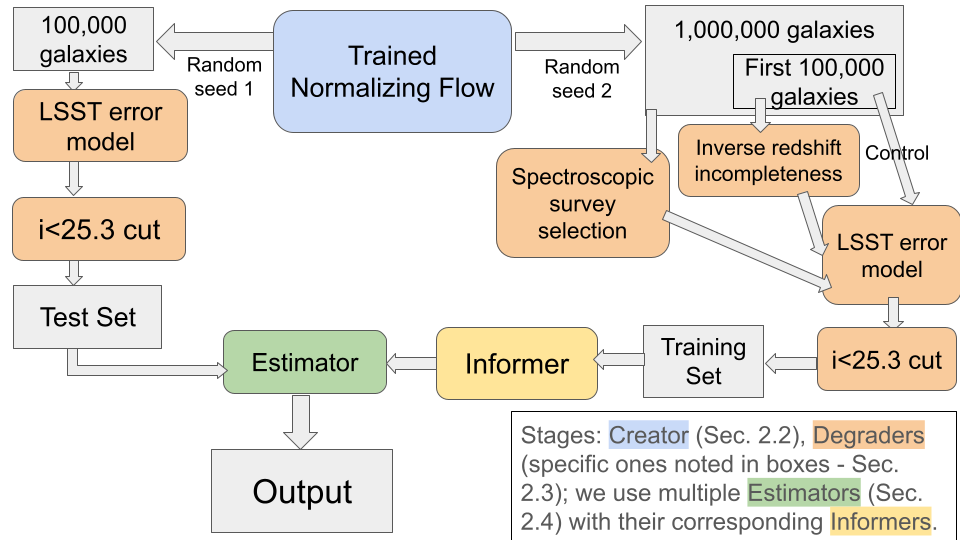
\includegraphics[width=0.75\textwidth]{RAIL_Pipeline_Workflow.png}
  \caption{A flowchart depicting the pipeline structure used to perform creation, degradation, and estimation. \refresponse{Boxes with rounded corners are RAIL stages, while boxes with sharp corners are data products.}
  Creation \refresponse{stages} are shown in \cwr{blue}, degradation stages in peach, the informer stage \refresponse{that trains a given photo-$z$ estimation method} in yellow, and the estimator stage in green. \refresponse{The sections where more information may be found for the RAIL stages used are indicated in the legend, and Sec.~\ref{sec:overview} describes the overall workflow in detail.}}
  \label{fig:pipeline} 
\end{figure*}

\section{Methods \& Data} \label{sec:methodsdata}

%\aim{I like at least outlining what readers will find in each subsection, but some folks leave it out.} 
Here we discuss the various features available in RAIL \refresponse{\citep{2025arXiv250502928T}} that have been employed in this work. 
In Section~\ref{sec:overview}, we summarize the pipeline structure used for our experiments.  We provide brief explanations of the simulated data in Section~\ref{sec:data} and our degradation methods in Section~\ref{sec:degraders}.
We provide visualizations of our degraded training data, and some relevant information on the surveys used to construct our spectroscopically degraded datasets. 
The photo-$z$ estimators we have examined are described in Section~\ref{sec:estimators}. 

\subsection{Overview of experimental design}
\label{sec:overview}

% \alice{will write this and try to make a flowchart with google draw or slides, or software from her tablet}

% \aim{I think most of this section can actually be the preamble of Section~\ref{sec:methodsdata} or split up among the subsections below rather than being repeated there.}


%\aim{It's needed, either here or earlier.
%I suggest moving what's above this point in this section to the introduction.}

%A pipeline of RAIL stages was constructed in order to enable the process of performing a large number of tests. The algorithms TrainZ, CMNN, GPz, PZFlow, and FlexZBoost were each tested on the same set of nine differently degraded training datasets. 

%For all estimators and all training sets, the same test set was used. 

Our experiment employs RAIL-based  pipelines to efficiently examine a large number of test cases\refresponse{, with a workflow shown in Fig.~\ref{fig:pipeline}}. We employ RAIL's dataset creation and photo-$z$ estimation subpackages, and perform evaluation externally to RAIL. 

In our creation phase, first, training and test set samples were drawn from mock data generated with the PZFlow implementation of a normalizing flow \citep{Crenshaw24}. This normalizing flow was trained on the Rubin-Roman simulation data (see Sec.~\ref{sec:data}). The same test set was used in all cases across all estimators \refresponse{(left branch of Fig.~\ref{fig:pipeline})}, while a large number of different training sets were \refresponse{created as in the right-hand branch of that figure and examined to understand the impact of different forms of spectroscopic incompleteness}. 


Our various training sets were obtained using different combinations of RAIL degradation stages. Our experiment \refresponse{was carried out using 3 types of training sets: training sets degraded with RAIL's inverse redshift incompleteness degrader, those degraded with spectroscopic selection from various surveys, and a control training set with neither form of degradation (designed to mimic the idealized case of a representative training set)}. \refresponse{For practical reasons, a larger initial pool of 1 million galaxies was needed when applying spectroscopic survey selections, as those severely downselect the galaxies, whereas the control and inverse redshift completeness training sets could be produced with a smaller initial population of $10^5$ galaxies.} 

\refresponse{As shown in Fig.~\ref{fig:pipeline}, after any other forms of degradation, all datasets  including the test set and control training set} were passed through RAIL's LSST error model degrader, \refresponse{applied with parameters corresponding to LSST 10 yr-depth \citep{ivezic2019}. The LSST error model stage interface through the Python package \texttt{PhotErr}, which is described in Appendix~B of \citep{Crenshaw24}.}
% \alice{TODO for Alex: cite relevant paper here}\aim{I think Ivezic 2009 is probably the right one}. 
This introduces realistic LSST-like error bars and noise into our data. Finally, we perform an $i$-band magnitude cut on all data, to avoid training and testing on objects that would not be selected for cosmological analysis with the LSST. 

In our estimation stage, each of the five estimators listed in Section~\ref{sec:estimators} were trained \refresponse{(the ``Informer'' stage)} on each degraded training set and the control training set, and tested on our standardized test set.
After our introduction of noise and magnitude cuts, our resulting test set contained approximately 31,000 galaxies.
The training set size varied based on the degradation method, with our smallest catastrophically incomplete case containing only 195 objects, and our largest training set containing over 80,000. \refresponse{A typical photo-$z$ training set needs to have on the order of 10,000 training galaxies \citep[page 12 of ][]{Newman2015}, therefore, we warn that the results with a smaller training set will suffer from sampling noise.  In a real survey, the size of the training set is usually larger than this size, so the results of extremely small training might not show a realistic effect. }

In order to analyze estimation results, a variety of different performance metrics were employed, discussed in detail in Section~\ref{sec:metrics}. Performance metrics were implemented outside RAIL infrastructure, with \texttt{numpy} (\citealt{NumPy}), \texttt{scipy} (\citealt{SciPy}), or by hand. 

%\aim{If this is the overview, you might want to say that you considered several metrics, but you don't have to say what they are here.}

\subsection{Data and sample selection}
\label{sec:data}

%\rachel{will ask Federico to describe the Rubin/Roman simulation}

% \subsubsection{Roman-Rubin Simulation}

\subsubsection{Truth catalog emulation}
\label{sec:truthcat}

Data from Tile 10307 from the Rubin-Roman simulation public data preview (\citealt{https://doi.org/10.26131/irsa569}; \citealt{2025MNRAS.544.3799O}) was used to train our normalizing flow. 
This data is reported in fluxes, as opposed to the magnitudes desired for this work, so all data was first converted to magnitudes using the standard SDSS definition of magnitude and LSST magnitude zero points. 
%\alice{cite this, and fact-check with TQ, Federico}
Tile 10307 contains approximately 3.5 million objects. 
Before training, all galaxies with \cwr{true} magnitudes fainter than 28 \cwr{in any band} were removed, leaving approximately 1.4 million objects. 
Of these remaining objects, 1 million were randomly selected and used to train the normalizing flow accessible through the RAIL creator stage employing PZFlow \citep{Crenshaw24}.

The normalizing flow is a sophisticated model for the joint probability density of redshift and magnitudes that we use as the basis for our mock data, which can be thought of as an interpolation of the seven-dimensional probability space of redshift and magnitude defined by the training set, which was the Roman-Rubin simulation in our case.
After generating a model with PZFlow's normalizing flow creator, initial training and test sets, comprised of true redshifts and magnitudes, were sampled. 
%\aim{Check colors vs. magnitudes as the data.} \alice{I'm quite confident it was magnitudes! As a user I've only worked with magnitude data when implementing PZFlow.}
%\tianqing{TODO for Alice: use a paragraph to talk about the true redshift. write this}
%\alice{conditional probability of redshift, given photometry. Do this with normalizing flow }
For our test set, 100,000 galaxies were sampled from the model, passed through the LSST error model with default parameters, and then subjected to an $i$-band magnitude cut of $i<25.3$. {We want to note that our flow models are trained on about 1.1 deg$^2$ of catalog, so we expect the truth catalog to have significant sample variance. } \refresponse{However, we do not expect the sample variance to significantly impact our conclusion. Future work is needed to propagate sample variance to the RAIL photo-$z$ results \citep{sanchez2020}.}

%\aim{I think the preceding to have significant sample variance.  two paragraphs can be deferred to \S~\ref{sec:degraders} if that section is reframed to be about degradation rather than the code itself.}
%\alice{talk about true posteriors}

\subsubsection{True posterior PDFs}
\label{sec:data:true_pdf}

In this work, we compare the estimated Probability Density Function (PDF) of the photo-$z$ to the ``true PDF'' of a galaxy. 
Normally, the true galaxy redshift would be one number. 
However, the concept of ``true PDF'' is physically motivated since a collection of galaxies at different redshifts could yield the exact same magnitude due to galactic physics. 
Therefore, we define the true PDF of galaxy redshift as the conditional probability distribution of redshift given the magnitudes in each band. 
%\aim{Was the PZFlow model defined in the space of colors or magnitudes? 
%I'm not sure we're consistent throughout the text\dots}
%\alice{Like above, I'm quite sure we defined the truth in magnitude space; I've not done anything as a user with colors. Furthermore the data is 7-dimensional (redshift and 6 magnitudes), and it would be 6-dimensional if we were working in color-space right?}
Statistically speaking, the true PDF of a galaxy with a set of magnitudes $m$ is
\begin{equation}
    P(z|m) = \frac{P(z, m)}{P(m)},
\end{equation}
where $P(z, m)$ is the joint probability density of the redshift-magnitude space, and $P(m)$ is the marginalized probability of the set of observed magnitudes $m$.  \cwr{In this work we are using a simulated dataset with some $P(z, m)$ that may differ in practice from realistic $P(z, m)$ due to uncertainties in galaxy populations and their evolution.  However, since we use the simulation for both training and testing set, any limitations in the simulated sample would apply to both and would not induce a training-testing set mismatch.}
% We use the PZFlow model for emulating the truth catalog to obtain the true PDF for each galaxy, as the PZFlow engine models the joint probability P(z, c) of the truth catalog. 

We obtained the true posteriors for our test set using RAIL's \texttt{FlowPosterior} stage. 
With its creation capabilities, PZFlow yields true model posteriors by evaluating conditional probabilities for each galaxy from the same joint probability space of redshift-magnitude data from which the actual redshifts and magnitudes of the test set were drawn. 
We provided PZFlow with our test set magnitudes, and used this functionality to generate our true redshift posteriors.;
as \texttt{FlowPosterior} generates unique conditional probabilities for each galaxy (as opposed to one single distribution applied to all galaxies), it obtains the true posterior for each galaxy from the cross-section of the conditional probability distribution $P(z|u_i,g_i,..., y_i)$ corresponding to its specific photometry. 
% \aim{Alice: I have made an attempt right before this comment. @alex please take a look and change things if needed!
% TODO for Alex: we'll need to describe the NF algorithm a little and the notion of the joint/conditional probability spaces to explain this}

\subsection{Training set degradation}
\label{sec:degraders}

% \aim{While degraders are the code structure used to implement these forms of training set imperfection, we might want to reframe this as forms of imperfection and then say in text how they were implemented with degraders.}

% \rachel{I will take the lead on fleshing this out}

RAIL's degradation algorithms are used to introduce systematic error into training sets of photometric data. 
Differences between training data and test data, such as training set incompleteness and non-representativity, affect photo-$z$ algorithm performance, but the specific training set conditions to which various estimation algorithms are sensitive or performant is not yet adequately understood. 
In this work, we \cwr{begin with a simple case of training set incompleteness at high redshifts in Section~\ref{sec:invz}.  We have next chosen} to examine the effects of training set degradation based on data collected by previous surveys, detailed in Section~\ref{sec:survs}, as existing survey data will likely be used in future science involving photo-$z$ estimation. 
 In all of these cases, we assume LSST-like photometric noise as described in Section~\ref{sec:lssterrmod}. \refresponsetwo{Note that in a real spectroscopic survey, the selections are done on photometry with noise from the corresponding imaging survey for the target selection. In this work, we ignored this photometric noise and assumed that the spectroscopic selection is done on perfect photometry, then applied the photometric noise degrader.} %\alice{This makes it sound a little like we are examining LSST-like noise separately from other degradation types. This is not exactly true; all of our data, including the control and test sets, went through the LSST error model degrader, so LSST error degradation was the baseline we compared everything else to.}. 

\begin{comment}
After the test set degradation described in Section \ref{sec:truthcat}, we were left with a dataset containing approximately 31,000 objects, each with a unique true posterior. 
For our control training set, the same degradation procedure was applied, but the initial 100,000 galaxies were sampled from the model with a different random seed, and true posteriors were naturally not generated. 

\refresponsetwo{The galaxy training set generated by the normalizing flow is degraded by one of two types of degraders.  The }

\refresponse{The galaxy training set generated by the normalizing flow is degraded by the following degraders:
\begin{enumerate}
    \item inverse redshift incompleteness (Section~\ref{sec:invz}): models for the spectroscopic incompleteness in the training galaxies,
    \item spectroscopic survey selection (Section \ref{sec:survs}): models for the selection functions in various spectroscopic surveys  
    \item LSST Error model (see Section~\ref{sec:lssterrmod}): LSST 10 year photometric error.
\end{enumerate}}

All training sets degraded with inverse redshift incompleteness followed this same procedure, but with the inverse redshift incompleteness degradation performed before the application of the LSST error model. 
This order was chosen only to reduce runtime; 
performing the inverse redshift incompleteness selection before LSST error degradation decreased the number of objects passing through the LSST error model.

For the training sets degraded with spectroscopic survey selection, a larger initial training set was necessary, as post-degradation datasets were too small to provide adequate training data otherwise. 
1 million galaxies were initially drawn from the model, then subject to the same series of degradations, with spectroscopic survey degradation in place of inverse redshift incompleteness. 
Again the order was chosen to decrease computational runtime, as the LSST error model stage takes longer to run than the spectroscopic survey degradation stages. 
This process is depicted visually in Figure~\ref{fig:pipeline}. {Note that in a real spectroscopic survey, the selections are done on photometry with noise from the corresponding imaging survey for the target selection. In this work, we ignored this photometric noise and assumed that the spectroscopic selection is done on perfect photometry.}
\end{comment}


\begin{figure*}
  \centering
  \includegraphics[width=1.0\textwidth]{Invz_Degradation.png}
  \caption{Regions in redshift-magnitude space  remaining populated after inverse redshift incompleteness degradation, performed with several different values of $z_0$ (as labeled at the top of each column). 
  The colormap indicates the density of surviving data, while the pink points have no inverse redshift incompleteness degradation and are our test set. \refresponse{The top 6 rows show the 6 LSST passbands, while the bottom row shows the 1D histograms of redshift before and after the degradation.} %\rachel{not sure what is meant by `test training set', should this perhaps be `control training set' or `test set'?} \alice{oops! Sorry, typo} (see Fig.~\ref{fig:pipeline}) . 
  }
  \label{fig:invz trainsets} 
\end{figure*}

\subsubsection{Inverse Redshift Incompleteness}
\label{sec:invz}

First introduced in \citet{Stylianou22},  \refresponse{the inverse redshift incompleteness degrader can be used to generate semi-realistic spectroscopic survey success rate which has lower completeness after a pivot redshift, either from fainter magnitude of the high-redshift galaxies, or that the spectroscopic features fall outside of the spectrograph’s wavelength coverage. } Inverse redshift incompleteness degradation is implemented as a function of some pivot redshift value $z_0$. 
Each galaxy in a dataset is assigned a survival probability as a function of this value, given by $1 - \text{min}(1, \frac{z_0}{z})$, where $z$ is the galaxy's redshift. 
Galaxies are then removed from a dataset according to this probability distribution, with the intent of replicating the incompleteness at higher redshifts seen in training data from real sky surveys. 
As \citet{Stylianou22} was completed before RAIL was released, we test the RAIL implementation with the same pivot values to confirm that we can recover results consistent with the original implementation, demonstrating the validity of our pipeline in the one case previously explored in the literature. We also include some higher values of pivot redshift in our work, in order to recover trends in performance as $z_0$ is changed. 
We test pivot values of $z_0 = \{0.1, 0.3, 0.6, 1.0, 1.4$\}. The impact of this degrader on the magnitude versus redshift relation is shown in Fig.~\ref{fig:invz trainsets}. \refresponse{The inverse redshift incompleteness skew the overall redshift distribution with different $z_0$ values. The $z_0 = 0.1$ model selects few objects overall due to an extremely low pivot redshift, although this is an extreme scenario. }
%\aim{Re: previous sentence, we don't actually know that until the results section so shouldn't mention it yet, just that we include this test for a reason.}

\begin{figure*}
  \centering
  \includegraphics[width=1.0\textwidth]{Spec_Survey_Degradation.png}
  \caption{Regions in redshift-magnitude space  remaining populated after spectroscopic survey degradation. 
  The colormap indicates the density of surviving data, while the pink data have received no spectroscopic survey degradation and are our test set (see Fig.~\ref{fig:pipeline}). Note the variation in degrees of test set coverage and localization of data in redshift-magnitude space across different surveys. \refresponse{The top 6 rows show the 6 LSST passbands, while the bottom row shows the 1D histograms of redshift before and after the degradation.}}
  % \tianqing{
  % (a) unify the x and y axes so the tick labels only shows once per column/row. 
  % (b) tick marks font size needs to be larger. 
  % (c) gap between panels needs to be smaller 
  % (d) the margin between labels and the panel needs to be smaller, 
  % (e) tick marks go inward. 
  % (f) label font size matches the manuscript's size. 
  % }
  %\aim{Suggestion: order the columns by number of galaxies for all the survey-specific cases.}}
  \label{fig:spec trainsets} 
\end{figure*}

\subsubsection{Survey-Based Degradation}
\label{sec:survs}

RAIL contains degradation stages designed to mimic the incompleteness and non-representativity patterns in spectroscopic data collected or used by past surveys. 
%\aim{I recommend putting these items in the same order as Figure~\ref{fig:spec trainsets}.}
We employed six such degraders: 
%\rachel{Still need to write HSC}
%Still need to write HSC. 
\begin{enumerate}
\item The Sloan Digital Sky Survey (SDSS) Baryon Oscillation Spectroscopic Survey (BOSS, \citealt{2013AJ....145...10D}): 
We use the target selection described in \cite{2016MNRAS.455.1553R}.  
BOSS is a wide-area survey targeting relatively bright, typically red, galaxies for the purpose of measuring large-scale structure rather than targeting a flux-limited sample for training photometric redshift methods, so it is particularly non-representative of anticipated LSST samples. 
Its spectroscopic success rate is very high, so the main impact of this degrader is to apply the targeting criteria to the photometry.\footnote{Caveat: Very few galaxies in our training data survive BOSS degradation, due to these heavy color and magnitude cuts. Due to its tiny size, one would expect estimates made using only BOSS training data to perform even more poorly by our metrics than those made with GAMA training data, so it is included in our analysis largely to contrast with GAMA. We recognize that both surveys result in catastrophically and unrealistically incomplete training data, however the ways in which some estimators respond to the two cases were surprising.} 
%\rachel{Need to motivate the `pseudo-BOSS' framing used in later figures, and also make those figures self-consistent (some say `BOSS' and others `pseudo-BOSS').}
%
\refresponse{Since our degrader implements an approximate version of the BOSS target selection, we refer to this case hereafter as `pseudo-BOSS'. }
\item The Galaxy And Mass Assembly (GAMA, \citealt{2022MNRAS.513..439D}) survey: 
This survey observed a relatively bright sample of galaxies (compared to LSST samples) over a few hundred square degrees.  
For this survey, we use the approximate 90\% completeness limit of $r<19.87$ and do not apply any spectroscopic incompleteness for the selected galaxies. 
%
\item The Hyper Suprime-Cam (HSC) survey \citep{2018PASJ...70S...4A}:
    Unlike the other degraders, this one is associated with a photometric survey (HSC), and corresponds to the merged spectroscopic sample used by the HSC team to train photometric redshifts.  It was implemented in \citet{2023ApJ...950...49M} as the union of multiple different spectroscopic surveys\footnote{For details of quality cuts imposed on the samples, please see \url{https://hsc-release.mtk.nao.ac.jp/doc/index.php/catalog-of-spectroscopic-redshifts__pdr3/}}, as described in \citet{2020arXiv200301511N}.  
    These include all of the above-mentioned samples for which there are individual degraders, though the HSC GAMA dataset is from an earlier release, data release 2 \citep{2015MNRAS.452.2087L}, and the HSC SDSS dataset is from a later release that includes the extended Baryon Oscillation Spectroscopic Survey \citep{2020ApJS..249....3A}.  
    It also includes the following additional samples: UDSz\footnote{\url{https://www.nottingham.ac.uk/astronomy/UDS/UDSz/}} \citep{2013MNRAS.433..194B,2013MNRAS.428.1088M}; 3D-HST\footnote{\url{https://archive.stsci.edu/prepds/3d-hst/}} \citep{2014ApJS..214...24S,2016ApJS..225...27M}; FMOS-COSMOS\footnote{\url{https://member.ipmu.jp/fmos-cosmos/FC_catalogs.html}} \citep{2015ApJS..220...12S}; VIPERS\footnote{\url{http://vipers.inaf.it/}} public data release 1 (PDR1; \citealt{2014A&A...562A..23G}); SDSS quasar sample from data release 14 \citep{2018A&A...613A..51P}; WiggleZ\footnote{\url{https://wigglez.swin.edu.au/site/forward.html}} data release 1 \citep{2010MNRAS.401.1429D}; DEEP3\footnote{\url{https://sites.uci.edu/deep3/}} \citep{2011ApJS..193...14C,2012MNRAS.419.3018C}; PRIMUS\footnote{\url{https://primus.ucsd.edu/}} data release 1 \citep{2011ApJ...741....8C,2013ApJ...767..118C}; the 2dF Galaxy Redshift Survey (2dFGRS\footnote{\url{http://www.2dfgrs.net/}}; \citealt{2003astro.ph..6581C}); the 6dF Galaxy Redshift Survey (6dFGRS\footnote{\url{http://www.6dfgs.net/}}; \citealt{2004MNRAS.355..747J,2009MNRAS.399..683J}); the Complete Calibration of the Color-Redshift Relation (C3R2\footnote{\url{https://sites.google.com/view/c3r2-survey/home}}) survey \citep{2017ApJ...841..111M,2019ApJ...877...81M}; the DEIMOS 10k sample \citep{2018ApJ...858...77H}; the Large Early Galaxy Census (LEGA-C\footnote{\url{https://www.eso.org/sci/publications/announcements/sciann17120.html}}) survey data release 2 \citep{2018ApJS..239...27S}; and VANDELS\footnote{\url{http://vandels.inaf.it/}} data release 1 \citep{2018A&A...616A.174P}. 
    In practice, this heterogeneous spectroscopic degrader applies both a cut on the photometry to reflect the targeting criteria of the spectroscopic datasets, and downsampling to reflect the spectroscopic success rate.  
    Both cuts are done in bins in the 2D space of $g-z$ color and $i$-band magnitude. 
    %
 \item The zCOSMOS survey: 
    We use the spectroscopic redshift success rate as a function of redshift and $i_\text{AB}$-band magnitude for the zCOSMOS-bright survey ($i_\text{AB}<$22.5) from the first two years of observations \citep[figure 3 of][]{2009ApJS..184..218L}.
\item The DEEP2 galaxy redshift survey \citep{2013ApJS..208....5N}: 
This survey covers 4 fields totaling 2.8 deg$^2$ down to $R_\text{AB}=24.1$.  
There are additional color cuts in three fields to target galaxy samples with $z \gtrsim 0.7$.  
While not precisely correct, the cuts on $B-R$ and $R-I$ in the DEEP2 targeting photometry are applied instead to $g-r$ and $r-i$ in our mock LSST dataset.  
The spectroscopic success rate is applied as a function of magnitude based on \citet{2013ApJS..208....5N}\footnote{Caveat: According to private correspondence with members of the DEEP2 team, the publicly available cut values may not be those that actually correspond to the survey data; as an official correction has not yet been issued, we nonetheless proceed with the posted values. \refresponse{We refer to our dataset implementing these cuts as 'pseudo-DEEP2' in order to avoid potential confusion.} 
%\aim{I took a stab at the caveat about the public-facing website the cut values came from and that it might differ from the actual survey}
}.
%\rachel{Need to forward-reference the `pseudo-DEEP2' framing used in later figures, and make them homogeneous in how they refer to this degrader.}
   %
    \item The VIMOS VLT Deep Survey (VVDS; \citealt{2013A&A...559A..14L} for the final release of the full survey): 
    We use the spectroscopic redshift success rate as a function of $i_\text{AB}$ in the range $[17, 24]$ from Figure~16 in \cite{2005A&A...439..845L} for the VVDS 2h field.  
    The redshift success rate is applied independently rather than jointly with magnitude, which results in a pessimistic view. This degrader results in a sample that is like some combination of the cuts for VVDS bright and VVDS deep rather than either alone due to $z$-dependent success rate.
%    
\end{enumerate}

%\aim{TODO for Alice: these vary in size by orders of magnitude. small training set size is also a form of imperfection!}

{We emphasize that our spectroscopic degraders are designed to approximate the photometric distribution of the target selection of spectroscopic surveys. The real spectroscopic success rate also depends on other galaxy properties such as star formation rate and stellar mass, which are not considered in this work. }

Referring to Figure \ref{fig:spec trainsets}, we see an illustration of the distributions of the corresponding surveys. Real spectroscopic success also depends on the physical properties of the galaxy, such as data from each of these surveys in redshift-magnitude space. The pseudo-BOSS survey represents a catastrophically poor training set case; it is both severely incomplete and not representative of the true distribution of galaxies in redshift-magnitude space. Though GAMA data is denser in the regions it covers, it also represents a very incomplete portion of our test data, with the vast majority of data concentrated below $z\approx0.7$ and a magnitude of 20. zCOSMOS is very complete for redshifts less than $z\approx1.5$, but contains no data for higher redshifts, and also lacks magnitude depth. pseudo-DEEP2 has good coverage of much of the test dataset, but has a large gap between $z\sim0.3$ and $z\sim0.6$, and less depth in magnitude. VVDSf02 and HSC are the most complete of the datasets examined here. The VVDSf02 training set contains the most data points, and they populate much of the redshift-magnitude space in our test set, though depth is slightly lacking in some bands. Though less dense than VVDSf02, HSC is the most representative of the surveys we examined, with data populating nearly all of the redshift-magnitude space covered by our test set.

The variety of different cuts described above produce significantly different post-degradation training set sizes (listed in leftmost column of Table \ref{tab:spec rej}), as stricter cuts cause more galaxies to be removed. The several surveys examined here provide us not only with variation in color and magnitude cuts, but also with significant variation in training set size, which is also a relevant form of imperfection. Our training set sizes vary from $\sim$200 objects (pseudo-BOSS) at the smallest to $\sim$80,000 objects (VVDSf02) at the largest. Though we recognize that training sets smaller than $\sim$10,000 objects (pseudo-BOSS and GAMA) are likely catastrophically and unrealistically incomplete, we examine both cases here, as some algorithms do not treat these two cases as we would expect. 

Though training set size is certainly a helpful form of imperfection to consider, it is also important to consider the distribution of training data in redshift-magnitude space relative to test data. For example, though our zCOSMOS case contains significantly more data than our HSC case, zCOSMOS data is densely isolated in a relatively small region of the redshift-magnitude space, whereas HSC data is spread over nearly all of the test set. 
Figure~\ref{fig:spec coverage} shows our attempt to quantify test set coverage under each type of survey degradation. Colored bars show the percentage of each band in our test set covered by each training set, while dashed lines show the average across all six bands for each survey training set. 
%\aim{TODO for Alice: move coverage section here}

\refresponse{We also note that a realistic training set for LSST will likely have spectroscopic and other reference samples from various sources matched to the photometric dataset, more like the HSC selection here and with of order $10^5$ galaxies.  Therefore, we do not expect the impact of the spectroscopic selection in a real survey to follow one of the single-survey selections, but rather the aggregate effect of all selections. }

\begin{figure}
\begin{center}
  \centering
  
\includegraphics[width=0.5\textwidth]{Coverage.pdf}
\caption{Bars correspond to approximate percentages of our test set covered by each spectroscopic training set, shown for each LSST band. The range of redshift-magnitude space captured in each band was covered with a discretized grid, with bins of width 0.1 in the redshift direction and 1 in the magnitude direction. The reported percentage is the percentage of the squares containing at least one test set galaxy that also contain at least one training set galaxy. Dashed lines correspond to the average coverage across all six bands for each spectroscopic degrader.}

\label{fig:spec coverage} 
\end{center}
\end{figure}


\subsubsection{LSST Error Model}
\label{sec:lssterrmod}


%\aim{cite the LSST Science Book (Ivezic 2009) rather than explaining the whole complicated equation}

Every training set used in our analysis was passed through the LSST error model degradation stage (section 3.2 of \citealt{ivezic2019}) after other degradation was applied, in order to approximate LSST-like photometric noise in training sets. Default parameters were used, corresponding to 10-year depth. 
%\rachel{Just to confirm: you used the default setting, corresponding to 10-year depth?  I think that is correct, but just want to check.  This should be stated explicitly.}\alice{Yes, we used default parameters!}

We also constructed a control training set using the LSST-like error as our only form of degradation. 
Every algorithm was trained once on a dataset designed to be representative of its test set, in order to provide a ``baseline'' for ideal training set conditions. 
Before making magnitude cuts, this data was degraded with the LSST error model only, and sampled from the same larger set of galaxies as the test set, using a different random seed. 

%\aim{This is a good place to introduce the idea of an experimental control that's representative but with the LSST error model degrader applied.}

\subsection{Estimators}
\label{sec:estimators}

% \aim{will take the lead on this: 
% Talk about different estimation algorithms briefly, and maybe why there are multiple. 
% Maybe state a hypothesis about which ones will perform best/reference previous results here. 
% (in each subsubsection, include discussion of the conditions under which we expect each to perform well/poorly)}


This study is not intended to be a comprehensive data challenge between all estimators under consideration for LSST;
rather, it is intended to examine how we can best assess the relative sensitivity of estimators as training set imperfection worsens, so we understand what test cases are meaningful and how to interpret assessment metrics in a full-scale, more realistic experiment with all estimators and their tuning parameters.
As a result, we have chosen a subset of photo-$z$ estimators representing categories of relevance\refresponse{:}
%
%\subsubsection{TrainZ}
%\label{sec:TrainZ}
%
\begin{enumerate}
    \item 
Our experiment uses \texttt{trainZ}, first introduced in \citeDCt, as an algorithmic experimental control. 
It assigns each test set galaxy a photo-$z$ PDF equal to the redshift distribution of the training set, without taking into account the photometry of the galaxies in the test set. 
{\texttt{trainZ} performs poorly in point estimate metrics and CDE loss}, yet it outperformed the real estimators by nearly all metrics in \citeDCt due to {the fact that the training set was representative of the test set. In this work, we expect \texttt{trainZ} to perform poorly due to the non-representative training set we employ. }
%
%\subsubsection{FlexZBoost}
%
\item \texttt{FlexZBoost} is a conditional density estimator introduced in \citet{Izbicki17} and demonstrated in the context of astronomy in \citet{Dalmasso20}.
It uses the distribution of training set galaxies close to each test set galaxy in color-space to approximate the distribution of redshifts of galaxies using a Fourier basis.
It is included in this study because it performed best by the only metric in \citeDCt that appropriately penalized \texttt{trainZ} and is thus likely to be used for LSST.
%
%\subsubsection{CMNN}
%
\item The Color-Matched Nearest Neighbor algorithm, implemented as \texttt{CMNN}, was first introduced in \citet{Graham18}.
It is included in this study because it is used throughout the \textsc{LSST} ecosystem for testing and optimization purposes, for example, for assessing the impact of observing strategy on photo-$z$ quality.
For each test set galaxy, \texttt{CMNN} identifies a subset of training set galaxies with similar colors and assigns the test set galaxy a photo-$z$ PDF equal to a Gaussian approximation to the redshift distribution of that set of galaxies;
for this reason, we will refer to it as a ``Gaussian estimator.''
\texttt{CMNN} differs from the standard k-nearest neighbor algorithm in that the subset is not defined as the fixed number k of nearest neighbors in the space of photometry.
Rather, the subset is defined by a distance that accounts for the observational errors of the test set galaxy, so the number of neighbors depends on the density of points in the training set as well as the precision of the test set galaxy's photometry. 
%
%\subsubsection{GPz}
%
\item Gaussian Process photo-$z$, implemented as \texttt{GPz}, models the space of photometry and redshift with a Gaussian process, as described in \citet{Almosallam15, Almosallam16}.
While the most up-to-date \texttt{GPz} applys a Gaussian process to the training set and evaluate a posterior PDF of a test set galaxy on a grid based on the same Gaussian process, \texttt{GPz} implemented in RAIL currently assumes the individual test set photo-$z$ PDFs are Gaussian distributions whose variances contain contributions from both aleatoric uncertainty due to the training set's sparsity and epistemic uncertainty due to the test set photometric errors;
% Similar to CMNN, GPz works in the same seven-dimensional color-magnitude space. Locating the points in this space given by test set photometry data, it draws a gaussian PDF estimate, based on the redshifts of weighted neighboring points. Thus GPz always gives gaussian outputs as its estimated redshift PDFs. 
we will also refer to \texttt{GPz} as a ``Gaussian estimator.''
\texttt{GPz} is included here to enable consistency checks with \citet{Stylianou22}, the only previous study to consider any of our test cases.
%
%\subsubsection{PzFlow}
% \label{sec:pzflow}
%
\item \texttt{pzFlow} \citep{Crenshaw24} models the joint probability distribution of photometry and redshift with a normalizing flow, an effective interpolation scheme of the seven-dimensional space.
Photo-$z$ PDFs are then evaluated as posteriors, at fixed photometry and evaluated on a grid of redshifts.
\texttt{pzFlow} is included in this study for self-consistency checks against the forward modeling approach, as the same underlying algorithm serves as the back-end for creating the mock data used for all test cases.
\end{enumerate}

\section{Performance Metrics}
\label{sec:metrics}

%In this section, we provide a brief explanation of each of the metrics used to assess our results.

% \tianqing{Should we have a subsubsection to introduce how ``true p(z)" is computed in this work?}
% \aim{Agreeing with TQ!





% I think it should go in \S~\ref{sec:data}.}


Various performance metrics 
% included in RAIL 
were used to examine the accuracy of the outputs of each algorithm under the chosen training set conditions. 
The use of several different performance metrics is important in our analysis in order to obtain a holistic understanding of algorithm sensitivity, as some metrics may not be able to detect the impact of imperfect training data 
% \rachel{not sure what is meant by `imperfect robustness'; reword?} 
while others could potentially flag opportunities for algorithmic improvement in this area.
All performance metrics were implemented with \texttt{scipy} \citep{SciPy} or \texttt{sklearn} \citep{scikit-learn}, or constructed by hand outside of RAIL infrastructure\footnote{Some of these are available in RAIL v1, a later version of the software than was used in this work.}. 

 Distribution-to-distribution metrics, described in Section~\ref{sec:distdist}, were used to compare estimator outputs \revone{}{$\hat{p}(z | x_{i}, \pi_{j})$ of redshift $z$ given the $i$th galaxy's photometry $x_{i}$ for each estimator $j$'s implicit prior $\pi_{j}$} to the test set true posteriors\revone{, and point-to-distribution}{ $p(z | x_{i})$.
\refresponsetwo{CDF-based metrics, described in Section~\ref{subsec:cdf}, were used similarly, but for cumulative distribution functions.}  Point-to-distribution
}
metrics, described in Section~\ref{sec:pointdist}, were used to compare to true (spectroscopic) redshifts also obtained from the test set. 
% Distribution-to-distribution metrics, described in Section~\ref{sec:distdist}, were used to compare estimator outputs to the test set true posteriors, and point-to-distribution metrics, described in Section~\ref{sec:pointdist}, were used to compare to true (spectroscopic) redshifts also obtained from the test set. 
Mode point estimates \revone{}{$\hat{z}_{i, j}$} obtained from estimator outputs \revone{}{$\hat{p}(z | x_{i}, \pi_{j})$} were also compared to the\revone{se}{ true (}spectroscopic\revone{}{)} redshifts \revone{}{$z_{i}$} using the metrics of Section~\ref{sec:outlier rejection}. 
%% \aim{I rearranged the subsubsections into the headings that were already outlined here, so you should check that it was done right.}

% \aim{We might want to divide the subsubsections into point-to-point, point-to-PDF, and PDF-to-PDF metrics rather than one metric at a time.
% This would also give the content in Section~\ref{sec:distshape} a better home, closer to the metrics it elaborates on without parts of it having to be repeated over and over again.}

\refresponse{In most cases, the detailed definition and implementation of the metric is described in Appendix~\ref{app:metrics}, and we summarize here the key aspects of the metric needed to understand the results.}

\subsection{Distribution-to-Distribution Metrics}
\label{sec:distdist}

%\aim{A brief preamble here is also a good place to reiterate where the notion of true PDFs came from.
%It would also be a good place to introduce the notation for true vs. estimated PDFs that's used in the definitions below.
%Also, you might want to make these equations on separate lines using the (commented out here) equation
% \begin{equation}
% \dots
% \end{equation}
%environment since they do get referred to again in \S~\ref{sec:pointdist}.}


%\aim{@alex how does this look for a preamble?}

Since we are able to generate true posterior distributions for our test data (see Section \ref{sec:truthcat}), it is valuable to compare \revone{}{each estimator's} output distributions to these true posteriors. 
Comparing \revone{distributions}{probability densities} to \revone{distributions}{probability densities} gives us the most complete picture of true algorithm performance, as whole distributions encode significantly more information than point estimates do. 
Though in some instances we may use point redshifts as our ``truth'' (see Section \ref{sec:pointdist}\revone{}{)}, under cases of realistic complexity it is rare that we will have access to spectroscopic point redshifts for all of our test data. 
\revone{It is also valuable to employ \texttt{RAIL}'s \texttt{FlowPosterior} stage in our work, as this new capability has not been explored much in previous work.}{}

% In our descriptions of distribution-to-distribution metrics below, we have used the notation $X_i(z)$ and $ x_i(z)$ to refer respectively to the PDFs in redshift space of our true posterior and estimated distributions, and $F_i(z)$ and $f_i(z)$ to refer to their CDFs. 
Both PDFs and \revone{}{their cumulative distribution functions (}CDFs\revone{}{)} may be obtained easily and efficiently from array-like statistical ensembles with the Python library \texttt{qp} \citep{malz_approximating_2018}.
\revone{}{It was also valuable to put into use \texttt{RAIL}'s \texttt{FlowPosterior} stage in our work, as this new capability has not been explored much in previous work.} \refresponsetwo{The distribution-to-distribution metrics we use are as follows:}

\refresponse{
\begin{itemize}
\item Root Mean Square Error (RMSE): The Root Mean Square Error, or Root Mean Square Deviation, is the quadratic mean of a set of differences between true values and predicted values. \refresponsetwo{As such, it is particularly sensitive to outliers.}
\item Kullback-Leibler Divergence (KLD): The KLD is another statistical \revone{distance}{measure of discrepancy}, used to measure the \revone{difference}{divergence} between a reference (true) probability distribution and \revone{a second}{an approximating} (estimated) distribution\revone{}{, in the form of the information lost by using the approximation instead of the truth}. 
\end{itemize}
}

    % \begin{equation}
    %  % \revone{
    %  % \frac{\text{max}(K)-\text{min}(K)}{n} \sum{K}  = \frac{\text{max}(K)-\text{min}(K)}{n} \sum_{i=1}^{n}X_i(z) \  \log\left(\frac{X_i(z)}{x_i(z)}\right)
    %  % }{
    %  \mathrm{KLD}_{i,j} = %\frac{\max_{k}\mathrm{KLD}_{i,j,k} - \min_{k}\mathrm{KLD}_{i,j,k}}{n} 
    %  \sum_{k=1}^{n} p(z_{k} | x_{i}) \ln\left[\frac{p(z_{k} | x_{i})}{p(z_{k} | x_{i}, \pi_{j})}\right]
    %  % }
    %  .
    %  \end{equation}
   % \aim{I took out something I didn't understand about the minima and maxima of the KLD values that I didn't understand but we should talk about before finalizing a resubmission.}
    % \begin{equation}
    %  % \revone{
    %  % \frac{\text{max}(K)-\text{min}(K)}{n} \sum{K}  = \frac{\text{max}(K)-\text{min}(K)}{n} \sum_{i=1}^{n}X_i(z) \  \log\left(\frac{X_i(z)}{x_i(z)}\right)
    %  % }{
    %  \mathrm{KLD}_{i,j} = \frac{1}{n}\left(\max_{k}\mathrm{KLD}_{i,j,k} - \min_{k}\mathrm{KLD}_{i,j,k}\right) .
    %  % \sum_{k=1}^{n} p(z_{k} | x_{i}) \ln\left[\frac{p(z_{k} | x_{i})}{p(z_{k} | x_{i}, \pi_{j})}\right]
    %  % }
     % \end{equation}
\subsection{CDF-based metrics}\label{subsec:cdf}
     
% \aim{these are dist-to-dist but get used for individual galaxies and ensembles.} \alice{?}

\revone{}{In our descriptions of metrics based on the CDF, the integral of a PDF, we denote the CDF of each galaxy $i$'s true and estimated posterior as $F_i(z)$ and $f_i(z)$ respectively.
When the CDF is estimated from samples, it is technically an empirical CDF (ECDF), which we denote as $\hat{F}(z)$ if it is derived from the true redshift posteriors and $\hat{f}_{j}(z)$ if derived from the $j$th estimator's redshift posteriors.
Both CDFs and ECDFs are obtained from the statistical ensembles output by RAIL stages using \texttt{qp} \citep{malz_approximating_2018}.} \refresponsetwo{The CDF-based metrics we use are as follows:}

\refresponse{
\begin{itemize}
\item Kolmogorov-Smirnov \revone{}{(KS)} Test Statistic: The KS defines a \refresponsetwo{maximum} distance between a \revone{cumulative distribution function}{CDF}, in our case \revone{the CDF}{that} of the true posterior generated for the test data, and an \revone{empirical distribution function}{ECDF}, in our case an estimator's output. \refresponsetwo{It is particularly sensitive to the central part of the distribution.}
\item Cramér-von Mises \revone{Criterion}{} (CvM): The Cramér-von Mises criterion is an alternative to the KS Test\revone{,}{ Statistic} in which the mean square distance between distribution functions is used\refresponsetwo{, potentially introducing sensitivity to other parts of the distribution beyond the center compared to the KS test}.
\item Earth-Mover's Distance (First Order Wasserstein Distance): The Wasserstein Distance is a measure of the distance-weighted integrated probability density of one distribution with respect to another distribution.
\end{itemize}
}
    
  
 
%The KS test can take on values between 0 and 1, with values closer to 0 indicating a more uniform PIT distribution. Therefore we expect more representative and complete training sets to yield lower KS test values. 

%We calculated this statistic using scipy.stats.kstest to compare the true CDF evaluated on a discrete grid to the estimated CDF, evaluated on the same grid. 

%\subsubsection{Cramér-von Mises (CvM) Criterion}
%The Cramér-von Mises criterion is an alternative to the KS Test, in which the mean square distance between distribution functions is used. Thus we also expect higher-quality training data to yield lower CvM values. Using the notation in Section \ref{ks}, the CvM criterion is defined as: 

%$\int_{-\infty}^{+\infty} [F_n(x) - F(x)]^2 \mathrm{d}F(x)$

%We calculated this statistic using scipy.stats.cramervonmises to compare the true CDF evaluated on a discrete grid to the estimated CDF.

% \subsubsection{Root Mean Square Error (RMSE)}

% \aim{fill in some technical info here}

% We used the mean squared error function in sklearn.metrics to compare the true PDF evaluated on a discrete grid to the estimated PDF, evaluated on the same grid. 

% \subsubsection{Kullback-Leibler Divergence (KLD)}

% \aim{fill in some technical info here}

% We used the KL-Divergence function form scipy.special to compare the true PDF evaluated on a discrete grid to the estimated PDF, evaluated on the same grid, element by element. Since the KL divergence is only defined for nonzero values, all zeros resulting in evaluating the PDFs over the chosen grid were set to $1\times10^{-300}$ . This resulted in a set $K$ of KL divergences for each galaxy. A continuity approximation was then made by hand via $\frac{max(K)-min(K)}{n} \sum{K} $, where $n$ is the number of elements in $K$. 

% \subsubsection{Wasserstein Distance}
% \aim{fill in some technical info here}
% \aim{This one wasn't included in RAIL, was it?}

\subsection{Distribution-to-Point Metrics}
\label{sec:pointdist}

Distribution-to-point metrics may be employed when true galactic redshifts are known to high enough precision that point estimates are appropriate, or in the absence of true posteriors with which to calculate distribution-to-distribution statistics. 
We examine two distribution-to-point metrics commonly referenced in previous literature. 
%\revone{In the descriptions below, we no longer employ the notation used in the previous section.}{\aim{I'm going to try to use the same notation as the previous section though there is a note here saying the notation will change.}}
%\aim{Briefly explain that the ``point" here is the truth and the estimates are PDFs, any new notation (z didn't appear above so some consistency should be enforced), and that the dist-to-dist metrics will be used again as meta-metrics.}

\refresponse{
\begin{itemize}
\item Probability Integral Transform (PIT): A statistic that quantifies whether the per-galaxy Bayesian posteriors are consistent with the corresponding population of true redshift values.
%\begin{description}
%    \item [Probability Integral %Transform (PIT)]
%    \label{sec:PIT}
%
%    \revone{For some random variable $X$ with a cumulative distribution function $F_{X}$, the}{The CDF $F_{Z}(z') = \int_{-\infty}^{z'} p_{Z}(z) \mathrm{d}z$ of a random variable $Z$ is itself a} random variable \revone{$Y := F_{X}(x)$ has a uniform distribution}{$Y:= F_{Z}(z')$}. 
%    In our case, estimators output Bayesian posteriors of the form \revone{$p = p(z\ |\ \mathrm{photometry})$}{$p(z | x_{i}, \pi_{j})$}, where the redshift $z$ is our random variable, from which \revone{cumulative distribution functions $F_z$}{per-galaxy CDFs $F_{Z_{i}}(z'_{i})$} may be obtained. 
%    If these posteriors are perfectly consistent with \revone{}{their corresponding population of} true redshift values, \revone{we may replace $z \rightarrow z_\text{true}$}{evaluation of each CDF at $z' = z_{\text{true}}$ yields values $y_{i}\sim Y_{i}$}, \revone{and}{where} the distribution of the random variable \revone{$Y := F_{z}(z_\text{true})$}{$Y$, known as the probability integral transform,} will be uniform. 
%    \revone{Thus we define a CDF for a single galaxy's distribution as\revone{: $ \int_{-\infty}^{z_\text{true}} {p(z\ |\ \text{photometry})\ } \mathrm{d}z$}{$\int_{0}^{z_\text{true}} p(z | x_{i}, \pi_{j}) \mathrm{d}z$},
%   and the distribution of such CDFs to be the PIT.}{} 
    We expect the PIT distribution for more representative and complete training sets to more closely resemble a uniform distribution. 
    Common features of non-representative PIT distributions are ``side spikes'' and ``middle bumps''\revone{: ``s}{.
    ``S}ide spikes'' indicate an over-abundance of instances where the truth is entirely on one side or the other of an output distribution, indicating that either \revone{estimates are wildly incorrect}{the bulk of the probability density is far from the true value} or that output distributions are too narrow. 
    ``Middle bumps'' indicate that the truth divides the output probability density roughly in half too often, indicating that an estimator may be over-fitting to training data or that output distributions are too \revone{narrow}{broad}. 
% \aim{A bit late for it, but science-wise, I think it would be valuable to evaluate the quantitative metrics below on the PIT curves relative to uniform to make more quantitative statements about the trends (and I think reviewers might ask for the same).}
    PIT distributions are compared to the uniform distribution using all the metrics of Section~\ref{sec:distdist}.
\item Conditional Density Estimate (CDE) Loss: The CDE Loss is an extension of the RMSE for PDFs that evaluates expectation values of the posterior PDFs of redshift conditioned on photometric data\refresponsetwo{, and is sensitive to outliers, scatter, and to a lesser extent biases in photo-$z$}. 
\end{itemize}
}
    
    
    %\item [Conditional Density Estimate (CDE) Loss]
%The CDE Loss is an extension of the RMSE for PDFs;
%instead of comparing true \revone{$X_{i}(z)$}{$p(z | x_{i})$} and estimated \revone{$x_{i}(z)$}{$p(z | x_{i}, \pi_{j})$} PDF values pointwise over $z$, the CDE loss evaluates expectations of the posterior PDFs of $z$ conditioned on photometric data \revone{$\xi$}{$x_{i}$} with respect to the \revone{}{population of} photometry \revone{$\Xi$}{$X = \{x_{i}\}$} and redshifts $Z$\revone{}{$= \{z_{i}\}$} of the test set data,
%\begin{equation}
% \mathcal{L} \equiv \mathbb{E}_{\Xi}\left[\int (x_{i}(z | \Xi))^{2} dz\right] - 2\mathbb{E}_{\Xi, Z}\left[x_{i}(Z | \Xi)\right] + K_{X_{i}} ,
%\mathcal{L}_{\mathrm{CDE}} \equiv \mathbb{E}_{X}\left[\int (p(z | x_{i}, \pi_{j}))^{2} dz\right] - 2\mathbb{E}_{X, Z}\left[p(Z | X)\right] + K ,
%\label{eqn:cde}
%\end{equation}
%\aim{I'd appreciate if someone could sanity check the above translation of notation!}
%for constant $K$ dependent on the true PDFs (which is thus dropped in calculation since it is the same across estimates).
%A more complete exposition of this metric can be found in \citet{Izbicki17}.
    % \aim{Big TODO for Alex: fill in technical info here}
%
%\end{description}

% \subsubsection{Probability Integral Transform (PIT)}
% \label{sec:PIT}

% For some random variable $X$ with a cumulative distribution function $F_{X}$, the random variable $Y := F_{X}(X)$ has a uniform distribution. In our case, estimators output Bayesian posteriors of the form $p = \mathrm{p(z\ |\ photometry)}$, where the redshift $z$ is our random variable, from which cumulative distribution functions $F_z$ may be obtained. If these posteriors are perfectly consistent with true redshift values, we may replace $z \rightarrow z_{true}$, and the distribution of the random variable $W := F_{z}(z_{true})$ will be uniform. 

% Thus we define a CDF for a single galaxy's distribution as: 
% $ \int_{-\infty}^{z_{true}} \mathrm{p(z\ |\ photometry)\ } dz$, and the distribution of such CDF's to be the PIT. 

% We expect the PIT distribution for more representative and complete training sets to more closely resemble a uniform distribution. Common features of non-representative PIT distributions are "side spikes" and "middle bumps": "side spikes" indicate an over-abundance of instances where the truth is entirely on one side or the other of an output distribution, indicating that either estimates are wildly incorrect or that output distributions are too narrow. "Middle bumps" indicate that the truth divides the output probability density roughly in half too often, indicating that an estimator may be over-fitting to training data or that output distributions are too narrow. 

% \aim{A bit late for it, but science-wise, I think it would be valuable to evaluate the quantitative metrics below on the PIT curves relative to uniform to make more quantitative statements about the trends (and I think reviewers might ask for the same).}

% \subsubsection{Conditional Density Estimate (CDE) Loss}

% \aim{fill in some technical info here}

\begin{figure*}
  \centering
  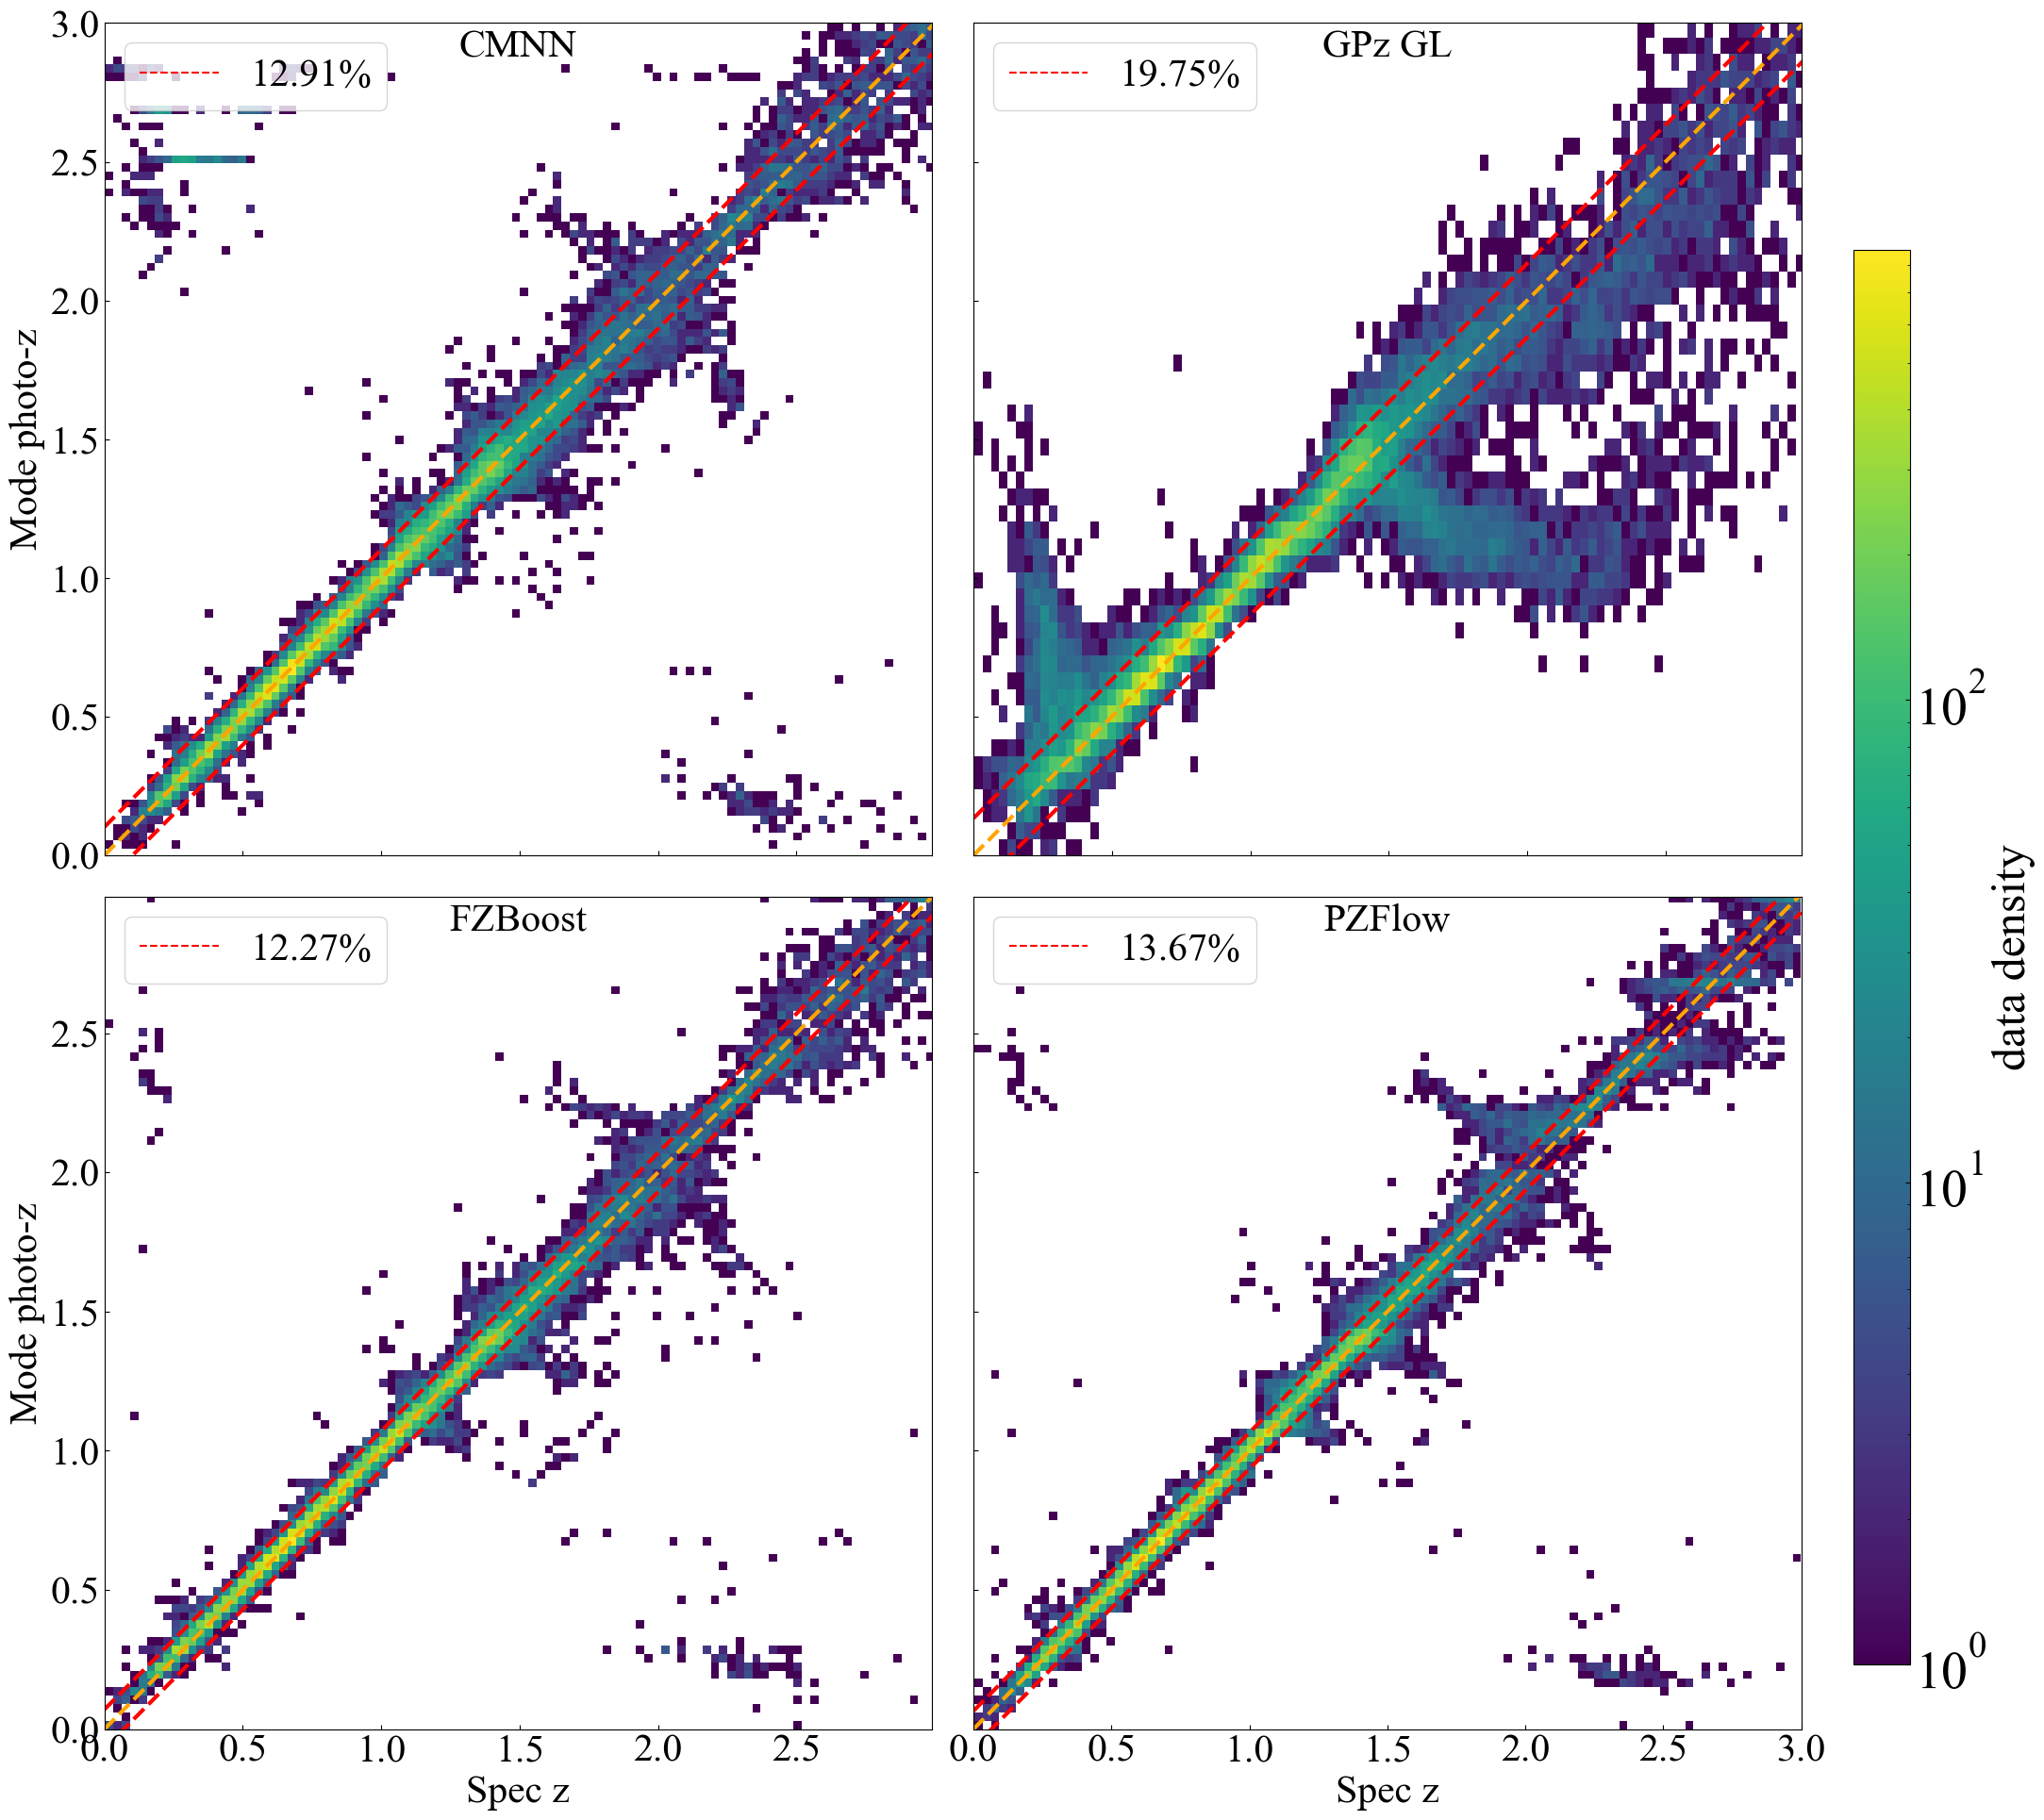
\includegraphics[width=0.8\textwidth]{Control_Modes.png}
  \caption{Mode point estimates obtained from estimator outputs under representative training conditions, versus true spectroscopic galaxy redshifts. Clustering along the diagonal is ideal case, which is shown by the dashed orange line. Red dashed lines show the 3$\sigma$ distance, calculated via outlier rejection. \texttt{TrainZ} is not shown, as the plot is not illustrative: it assigns every galaxy the same distribution, thus all modes are the same. $>3\sigma$ outlier rates are shown in the upper left corner of each panel. 
  }

  \label{fig:control modes} 
\end{figure*}

\subsection{\revone{Ensemble}{Point-to-point} Metrics}
\label{sec:pointestmets}

%\begin{description}
  %  \item[%Outlier \revone{Rejection}{Identification}]
    \refresponsetwo{One approach to quantitatively characterizing catastrophic outliers in the photo-$z$ point estimates is to statistically identify outliers and exclude the flagged outliers from further analysis.  Here we use the following algorithm:} 
    For a set of numbers, its mean and standard deviation are calculated. 
    Any elements greater than 3 standard deviations from the mean of the dataset are then \revone{labelled}{labeled} as catastrophic outliers and `rejected'. 
    The mean and standard deviation of the remaining dataset is then recalculated, and the process repeated recursively until convergence is reached and no more points are being rejected. 
    The rejected points are the catastrophic outliers of the dataset.
    We have implemented this metric by hand. 
    
    We use outlier \revone{rejection}{identification} to assess the mode point estimates obtained from estimator output PDFs. 
    For each data point in the plots of photo-$z$ mode versus spec-$z$ (for example, see Figure~\ref{fig:control modes}), its distance from the diagonal was calculated, and outlier \revone{rejection}{identification} was then performed on this set of distances in order to obtain a catastrophic outlier rate. 
    Though this metric is helpful in quantifying cases of extreme error, it is important to note that it can be easily biased by datasets with very large standard deviations, and the result will be artificially low in such cases. 
    \texttt{trainZ} is a prime example of this; as every point estimate for \texttt{trainZ} is the same, the standard deviation of the set of their distances from the diagonal is very large, thus nearly all points fall within $3\sigma$ of the diagonal. 
    We see this also in some cases of catastrophically poor estimation. 
    \label{sec:outlier rejection}

%\rachel{How was this implemented?  Did you use a standard package for this or implement it by hand?}

    %\aim{This is a good place to mention that when the point estimates are all way far from the truth (\trainz), the standard deviation is very large so the outlier rate will appear to be low, even though a high outlier rate is considered the sign of something being wrong \textemdash this is very counterintuitive to folks who've been using the $3\sigma$ outlier rate as a metric of point estimates for the past couple decades.}
    %\aim{On that note, I think readers familiar with the $3\sigma$ outlier rate might have the following thought: 
    %``huh, I never tried it with anything other than 3 and see that 5 is telling a different story from the intuition I built using 3.
    % I wonder what happens if you use other values in between."
    %So, it might be worth showing 1, 2, and 4 as well so they get an answer to that question of whether the other values tell us something different in terms of the connection between the plots like Figure~\ref{fig:control modes} for all the test cases and those like Figure~\ref{fig:invz rej}.}

%\end{description}


\begin{figure*}
  \centering
  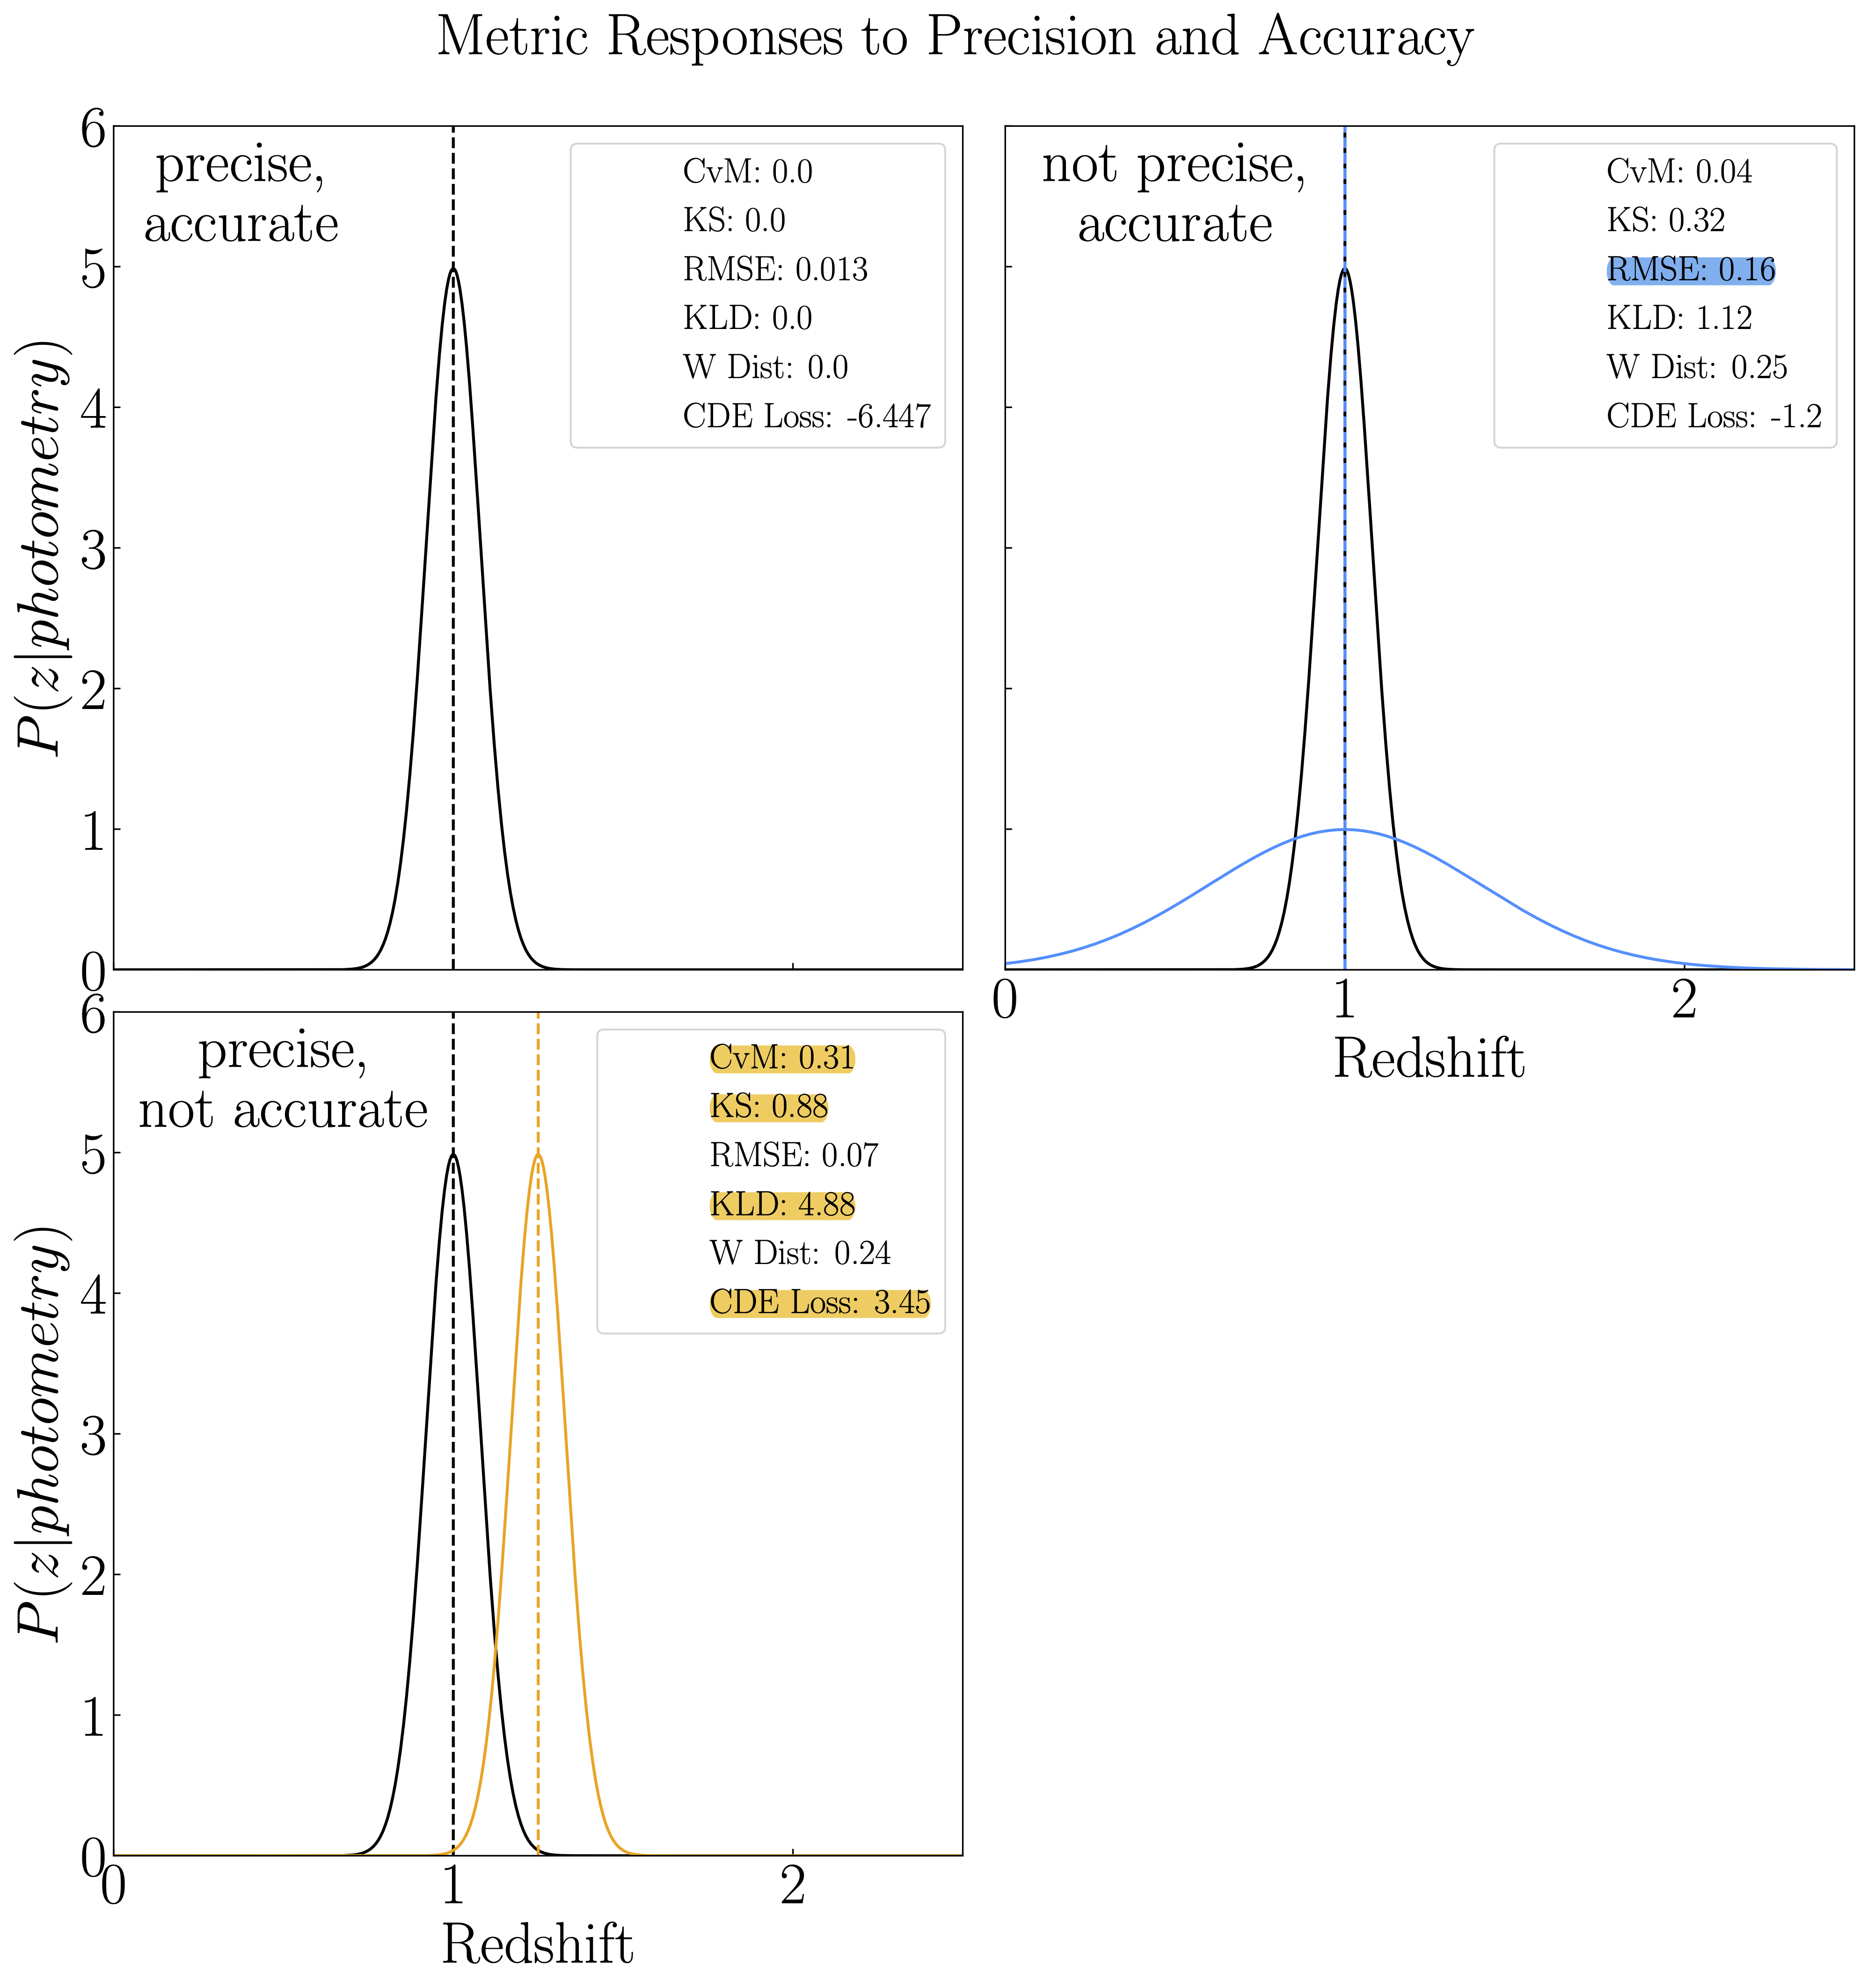
\includegraphics[width=0.65\textwidth]{distribution_stats_plot.png}
  % \caption{Here, example distributions are shown as a comparison of the effects of distribution shape on our five examined distribution-to-distribution statistics and two of our point-to-distribution statistics. All distributions shown here are gaussian. In the top left panel, distances between the black curve and itself are shown. The other panels show the distances between the black curve and each of the colored curves, providing an illustration of how each statistic behaves under accurate but imprecise, inaccurate but precise, and both inaccurate and imprecise conditions.
  % In the distribution-to-point statistics (CDF and CDE Loss), the mean of the black distribution (black dashed line) is used as the truth. We note the significant variation across the different cases in the majority of our statistics, many of which behave in different or opposite ways under shifts in distribution shape, illustrating the need for multiple metrics. The  }
\caption{Illustration of distribution-to-distribution metric responses to bias on the centroid and width of the distribution. 
Each panel shows the reference redshift distribution (black) alongside an altered version, representing scenarios with increasing scatter (top right), and biased centroid (bottom left). 
The numerical values of these statistics are shown in each panel to illustrate how they respond to different types of distributional changes. \cwr{The Wasserstein distance responds similarly to imprecision as to inaccuracy. The highlighted metrics in the legend indicate the cases where a metric is more sensitive to inaccuracy or to imprecision.} }
% The scenario\revone{s where}{ to which each} metric\revone{s are}{ is} most sensitive to \revone{are}{is} highlighted.}


 
  \label{fig:stdev fx} 
\end{figure*}

\subsection{Understanding the Metrics}
\label{sec:distshape}

% In our analysis, we find that several of our examined statistics are \refresponse{highly sensitive to the shape of the output $p(z)$ distributions, evincing a richness inherent to the distribution-based metrics relative to point estimate metrics}.  
% Despite producing mode point estimates that can be very close to true redshift values, excessively narrow output distributions often result in large values of the CvM, KLD, and CDE loss, while a distribution's CDF can be skewed towards being either very large or very small, depending on its location.
% This is illustrated in Figure~\ref{fig:stdev fx}\revone{}{ by evaluating the metrics for approximating distributions to a toy true distribution to build intuition for the behavior of the metrics, where the PIT is reduced to a single CDF value since there is only one approximation to a single fiducial distribution to consider; 
% PIT distributions are distributions of CDF values, thus we show the CDF of the approximating distributions at the mean of the black distribution, taken to be our ``truth''}.

\revone{}{In Figure~\ref{fig:stdev fx}, we illustrate how the distribution-based metrics react to two types of mischaracterization of the true PDF -- (a) overall bias in the distribution, (b) difference in the width of the distribution. }

\revone{}{The top left panel of Figure~\ref{fig:stdev fx} shows the distribution-based metrics comparing the PDF to itself. In this case, the CvM, KS, KLD, and Wasserstein distance are exactly zero. The RMSE is approximately $2 {\rm Var}[X]$, as predicted by its definition, which in this case is $2\times (0.08^2) = 0.0128$. The CDELoss is a negative value. }

\refresponse{Moving to the bottom left panel, w}e see that \revone{}{bias} between distributions is penalized heavily in the CvM, KS, KLD and CDELoss. 
It is penalized less in the RMSE, which is expected given the findings in \citet{malz_approximating_2018} \revone{which}{that} indicate relative insensitivity of the RMSE to distribution tails when compared with the KLD. 
Conversely in the KS test, similarity in shape rather than overlap results in a lower value\revone{}{, which makes sense since it is sensitive to the largest discrepancy in ECDF.  In the inaccurate case, that will just be a constant shift related to the area under one distribution where the other has zero probability, whereas in the imprecise case, it will depend on the slope of the CDF that comes from how much broader the approximating distribution is}. 

\revone{}{Overall, \cwr{the illustrated cases of inaccuracy and imprecision result in roughly the same Wasserstein distance, while the RMSE is more sensitive to an incorrect width of the distribution (top right panel), and the CvM, KS, KLD and CDELoss are more sensitive to biases (bottom left).
Furthermore, the dynamic range of each metric varies significantly, as the PIT/CDF, and KS are limited to [0,1], and the CvM, KLD, RMSE, and CDELoss have far more freedom.}
We also note that RMSE and Wasserstein distance have dimensions of redshift, while others are dimensionless, which makes the level of significance further incomparable between the metrics.}
This \cwr{figure} illustrates well the need for several different metrics to assess performance\revone{}{, and shows that any attempt to construct a ``super-metric" from a combination of these metrics should be done with extreme care if at all}. 

%% Rachel commented this out because it seemed to be talking about another figure (not sure which one) or an old version of this figure.  But it wasn't related to the rest of the section.
%\revone{}{PIT distributions are distributions of CDF values, thus we show the CDF of colorful distributions at the mean of the black distribution, taken to be our ``truth''.} 
%The \revone{orange}{inaccurate but precise approximating} distribution would end up in a ``side spike'' (see Sec.~\ref{sec:PIT}) on a PIT distribution, deviating far from uniformity. 
%With the CDE loss metric, again we see that very narrow, shifted distributions inflate the value of the statistic, despite being very close to the target distribution. 
%Conversely, for the CvM and KLD statistics, wide, flat distributions may produce a low statistic value, yet \revone{contain little to no information about an estimated redshift distribution and produce very inaccurate point estimates}{are relatively uninformative about redshift, with the potential for high variability in point estimates}. 

%\alice{read and cite \citet{malz_approximating_2018} to motivate this and back up observation that RMSE is not useful}

\section{Results \& Discussion} \label{sec:results}

%\aim{These next two paragraphs should go in the metrics section (\ref{sec:metrics}) because they're establishing intuition for the behavior/sensitivity of the metrics rather than analyzing the results of your experiments with data.}

Below we examine in detail the \revone{results}{values} obtained for \revone{each estimator using}{} each metric \revone{}{as evaluated over each estimator's $p(z)$ results for many cases of training set imperfection}. 
\revone{We divide our analysis into two sections, considering inverse redshift incompleteness and spectroscopic degraders separately.}{}
We discuss which metrics expose (or do not expose) particular trends in performance, and which are systematically biased (or unbiased) by distribution shape. 
We ultimately seek to identify which \refresponse{set of} metrics provide the most complete picture of photo-$z$ algorithm performance in our examined cases, rather than to identify (or tune) a ``best'' algorithm. 
Our list of photo-$z$ algorithms is not exhaustive, nor do we manipulate any algorithmic tuning parameters, thus we wish to emphasize that our work serves as an exploration of how one should evaluate estimators under various data challenge conditions. 
\revone{}{We divide our analysis into two sections, considering inverse redshift incompleteness and spectroscopic degraders separately.}

%\aim{You can just outline which questions will be answered in each of the subsections in this section.
%This is particularly important in setting the tone for how your results should be interpreted.
%You can take this opportunity to remind them that this is not a data challenge about choosing a ``best" estimator (when these are not an exhaustive list, you're not optimizing the parameters of the estimators, and the data isn't hyper-realistic) but rather an exploration of how one should evaluate estimators under data challenge conditions to make that assessment.}

%\subsection{Experimental Controls}
%\label{sec:res-controls}

%In order to understand baseline algorithm performance, multiple experimental controls were used in this analysis. 
%As discussed in \ref{sec:TrainZ}, the TrainZ algorithm makes estimations without considering at all the photometry of the data on which it is being tested. The hope is that all other algorithms significantly outperform TrainZ in reproducing true posteriors. 

%\aim{I think it's okay to only say this in Section~\ref{sec:TrainZ}.}

%In addition to an algorithmic control, training set controls were also used. 

%\aim{I think it's okay to only say this in Section~\ref{sec:lssterrmod}.}


\subsection{Inverse Redshift Incompleteness Effects}

We begin by examining the effects of the inverse redshift incompleteness degradation stage, as a toy example of spectroscopic degradation. As the effects of this stage have been examined before, we perform this analysis largely with the goal of reproducing conclusions drawn in previous work. In \citet{Stylianou22}, the authors analyze the performance of \texttt{GPz} under inverse redshift incompleteness degradation. We reproduce this analysis, as well as examining the performance of our other estimators under this form of degradation. 

%\aim{(Apologies if this comment is irrelevant because it's stated elsewhere \textemdash I'm reading out of order.) Before diving into the results, this is a good place to say you looked at this toy degrader to check consistency with a case that has been investigated before for one of the same estimators, as a reason for readers to be very confident in the rest of your results.}

\begin{figure*}
  \centering
  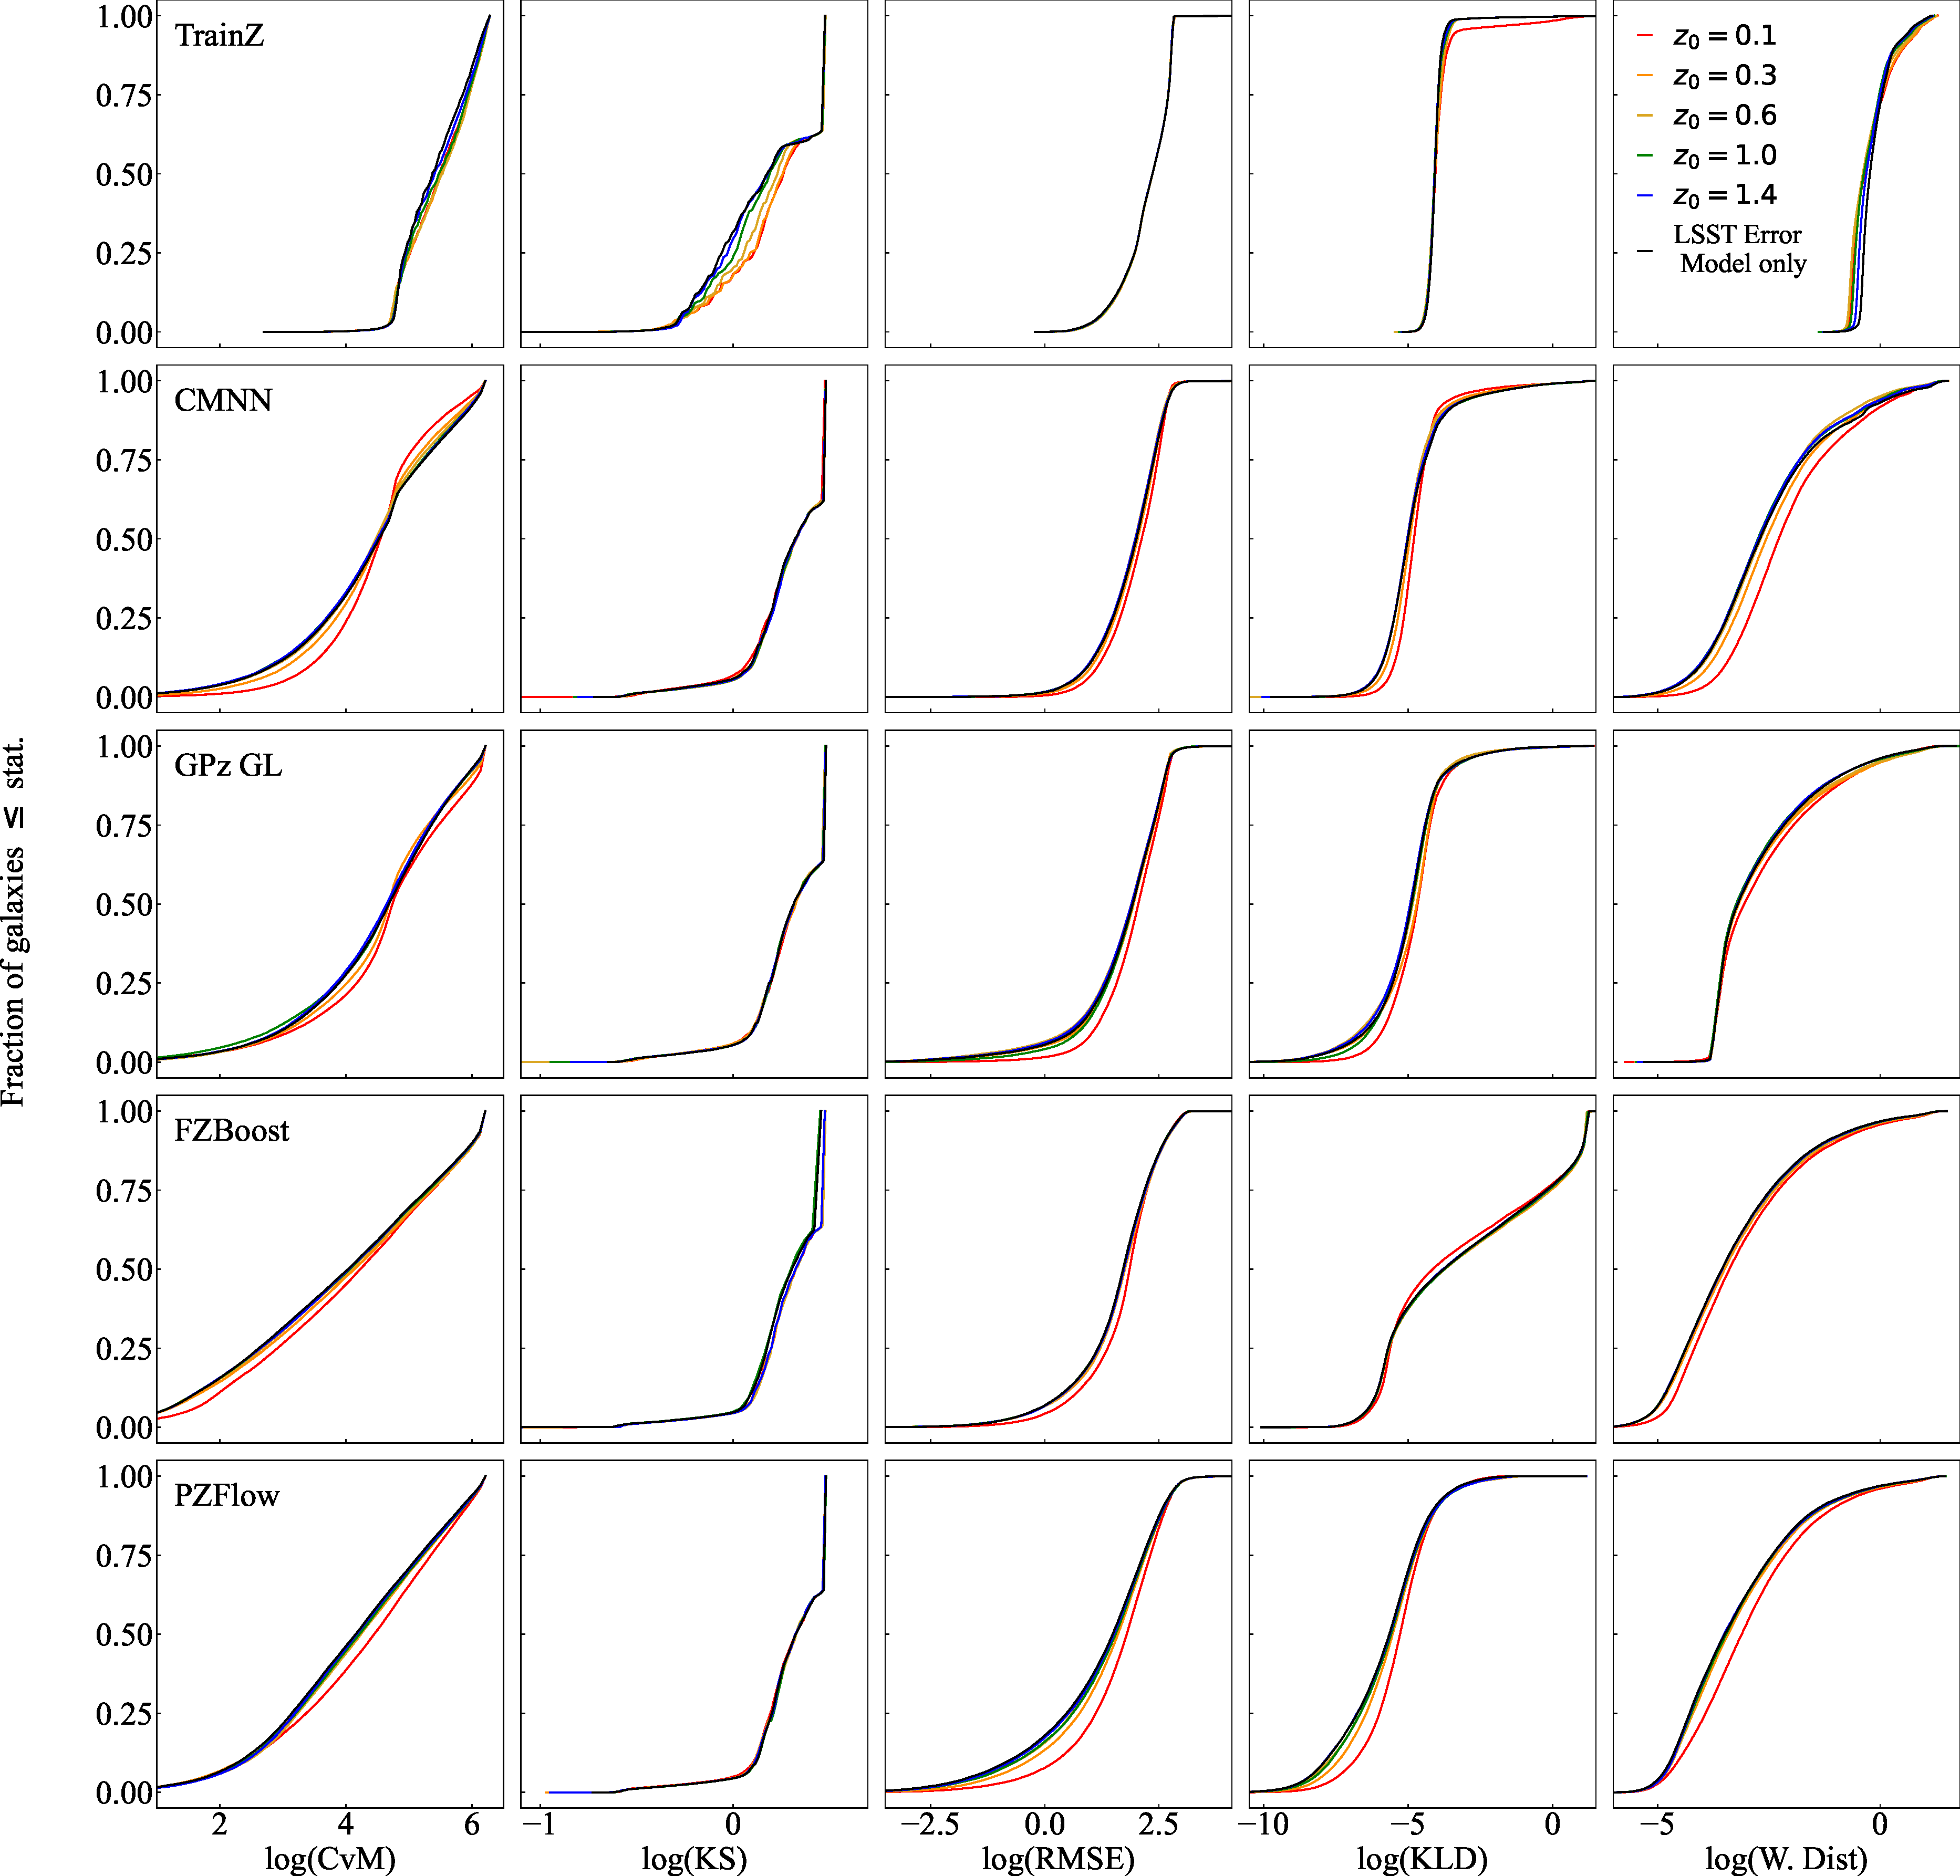
\includegraphics[width=1.0\textwidth]{Invz_D2D.pdf}
  \caption{Quantile plots of the distributions of logarithmic CvM, KS, RMSE, KLD, and Wasserstein Distance statistics (columns) for each photo-$z$ estimation algorithm (row), under various degrees of inverse redshift incompleteness severity (different colored curves in each panel). 
  The $y$ value for each point on a curve is the fraction of outputs with a statistic value less than or equal to its corresponding $x$ value. 
  Rapid increases in slope correspond to a large number of galaxies having the same statistic value. 
  We expect cases with more severe degradation to have higher overall statistic values, and thus steeper slopes towards the right side of their axes. We note that these metrics expose very little difference in performance as $z_0$ is varied, with the exception of the most severe cases of $z_0=0.1$.
  %\aim{might remake as difference from error model only?} \alice{Sorry, I don't quite understand what you mean here @alex} \rachel{Alex means that instead of plotting all CDFs, plot the difference between each CDF and the `LSST Error Only' CDF.  That way, instead of plotting a lot of curves that all look fairly similar, you are plotting something that makes differences evident.  In the context of the `LSST Error Only` curve being an experimental control, I think this makes a lot of sense.}
  }
  \label{fig:invz d2d} 
\end{figure*}

\subsubsection{CvM, KS, RMSE, KLD, W.\ Distance}

We find that the effects of inverse redshift incompleteness degradation on the majority of distribution-to-distribution statistics are minimal, across all photo-$z$ estimators. 
Our distribution-to-distribution statistic results are summarized in Figure~\ref{fig:invz d2d}, which shows the CDF of the distribution of per-galaxy values for each metric and photo-$z$ estimator. 
Comparing across \revone{panels in a fixed}{each} row \revone{provides a comparison between the results of different statistical tests}{shows the behavior of each metric} for a \revone{particular}{given} algorithm\revone{}{, whereas comparing down each column shows how a single metric differs between algorithms}. 
\revone{}{At first glance, Figure~\ref{fig:invz d2d} shows that for most metrics, there is greater sensitivity to photometric redshift algorithm than to the degree of inverse redshift completeness degradation of the training set.}

% \aim{Just a suggestion to highlight that this isn't a competition: Comparing across rows isn't as significant as comparing across columns in the same row.}

%Examining row 4, we see that FlexZBoost statistics are negligibly affected in all but the most severe case of $z=0.1$. 

%In row 5, PzFlow results are similar, with slightly more variation in the KS statistic. 
%We see a slight separation of the curves, with those corresponding to lower values of $z_0$ found preferentially towards the right, as expected. 

%\aim{I would recommend moving the last three sentences of this paragraph to the end of this subsection.}

%\aim{It might be good to rearrange (and just break up) this long paragraph by starting with what you see for the experimental control of TrainZ, then move on to how the real estimators differ.}

Examining row 1, we see how the different statistics \revone{examined}{considered} here characterize \texttt{TrainZ} performance. Little variation across different values of $z_0$ is seen, with only the most severe cases (low $z_0$) causing notable deviation in the \revone{CvM}{KS test}. Comparing the top row against other rows, we see that as we expect, statistic values for \texttt{TrainZ} are higher overall than those of our non-control estimators in the \revone{KS}{CvM}, RMSE, KLD, and W.\ Distance, but surprisingly slightly lower in the KS test. \texttt{TrainZ}'s apparent `good' performance in this statistic is a prime example of why using multiple performance metrics is important in assessing photo-$z$ estimator performance. 

%\alice{Since the new results have such limited differentiation between different values of $z_0$ and even between different estimators, I really don't think it makes sense to have an individual paragraph for each estimator. I'm going to pick out some features that are noticeably different and discuss those instead.}

\revone{}{Across our other estimation algorithms, shown in rows 2-5, these metrics illustrate remarkably little difference in performance for different $z_0$ values, with only the most extreme cases of degradation being distinguished.  The KS test appears to hardly differentiate at all between any levels of inverse redshift incompleteness. We note the significant spike at high KS values, indicating a pileup of cases in which this statistic indicates poor performance. This spike likely contains a combination of true catastrophic outliers and distributions that are narrow and slightly offset from the truth and thus yield artificially high KS test values. 
As both situations result in output distributions with little to no overlap with the truth, they both yield near-maximum KS values.}

% RM: I commented out the paragraph below because it was more about the estimators than the ability of the metrics to serve as useful diagnostics.
%\revone{}{Little else shown by these metrics distinguishes our test cases and estimators from each other. We note that the CvM distributions for CMNN and GPz appear to have inflection points, unlike the distributions for the other estimators. We also note the unique shapes of FlexZBoost's KLD curve and GPz's W. Distance curve when compared with the more sigmoid curves for other estimators in these two statistics. Aside from these few exceptions, these metrics show that our estimators are remarkably little affected by inverse redshift incompleteness, and that our non-control estimators perform similarly to each other across these metrics. }  
%Our Gaussian estimators, \texttt{CMNN} and \texttt{GPz} (rows 2 and 3), show minor variations between $z_0$ values across most metrics (with the exception of the KS test), though again these tests are only sensitive to the most severe degradation. Aside from this, differentiation between We note the significant spike at high values, indicating a pileup of large CvM values. This spike likely contains a combination of true catastrophic outliers and distributions that are narrow and slightly offset from the truth and thus yielding artificially high CvM's. As both situations result in output distributions with little to no overlap with the truth, they both yield near-maximum CvM values, despite the fact that catastrophic outliers are much more distant from the true distribution. 

%With \texttt{CMNN}, we see that all CvM distributions have very similar shapes, yet some of the cases where we expect poor performance are shifted towards lower values. When examining the effects of different toy Gaussian distribution shapes on the CvM statistic, we find that widening a distribution without shifting its mean with respect to our ``truth'' distribution results in a slightly lower CvM value, as this results in more tail overlap. When examining \texttt{CMNN} outputs by eye, we see that a primary difference between output distributions as $z_0$ is changed is their standard deviation, with lower values of $z_0$ corresponding to wider distributions. The CvM statistic reflects this shift effectively, yet gives a misleading representation of overall success. 

%In the case of \texttt{GPz}, we also see differentiation between $z_0$ cases in the CvM test, though the trend is largely as expected. We agree with \citet{Stylianou22} that we see a trend in increasing CvM values for more severe degradation, though it is mild. As cases with less severe degradation exhibit a spike at high CvM values, we conclude that narrow, slightly offset output distributions are common under these conditions, and less so in cases of more severe degradation. We also agree that there are mild trends of worsening performance as $z_0$ is decreased in the other statistics, though none is extreme. Consistency with prior results for \texttt{GPz} is encouraging, and lends credibility to the methods used to obtain our newer results. 


%\aim{This is also a good place to say, ``And now that we've shown consistency with prior results, you can trust us on the rest of this that has never been done before."}


%\aim{Explain what this means in terms of the CDF, i.e. how a distribution (PDF) with or without a spike looks.}

%Examining row 4, we see that \texttt{FlexZBoost} appears to be  affected remarkably little by inverse redshift incompleteness degradation. None of the distribution-to-distribution statistics examined here reflect much worsening in performance as $z_0$ is decreased, with the exception of very slight separation of the curve corresponding to the most severe case from the others. 

%\texttt{PzFlow} also exhibits little variation across test cases, particularly in the CvM test, which reflects very little change in performance for either \texttt{FlexZBoost} or \texttt{PzFlow}. Across the other statistics, the only case showing significant deviation from the others is the most severe $z_0 = 0.1$ case. 




\begin{figure*}
  \centering
  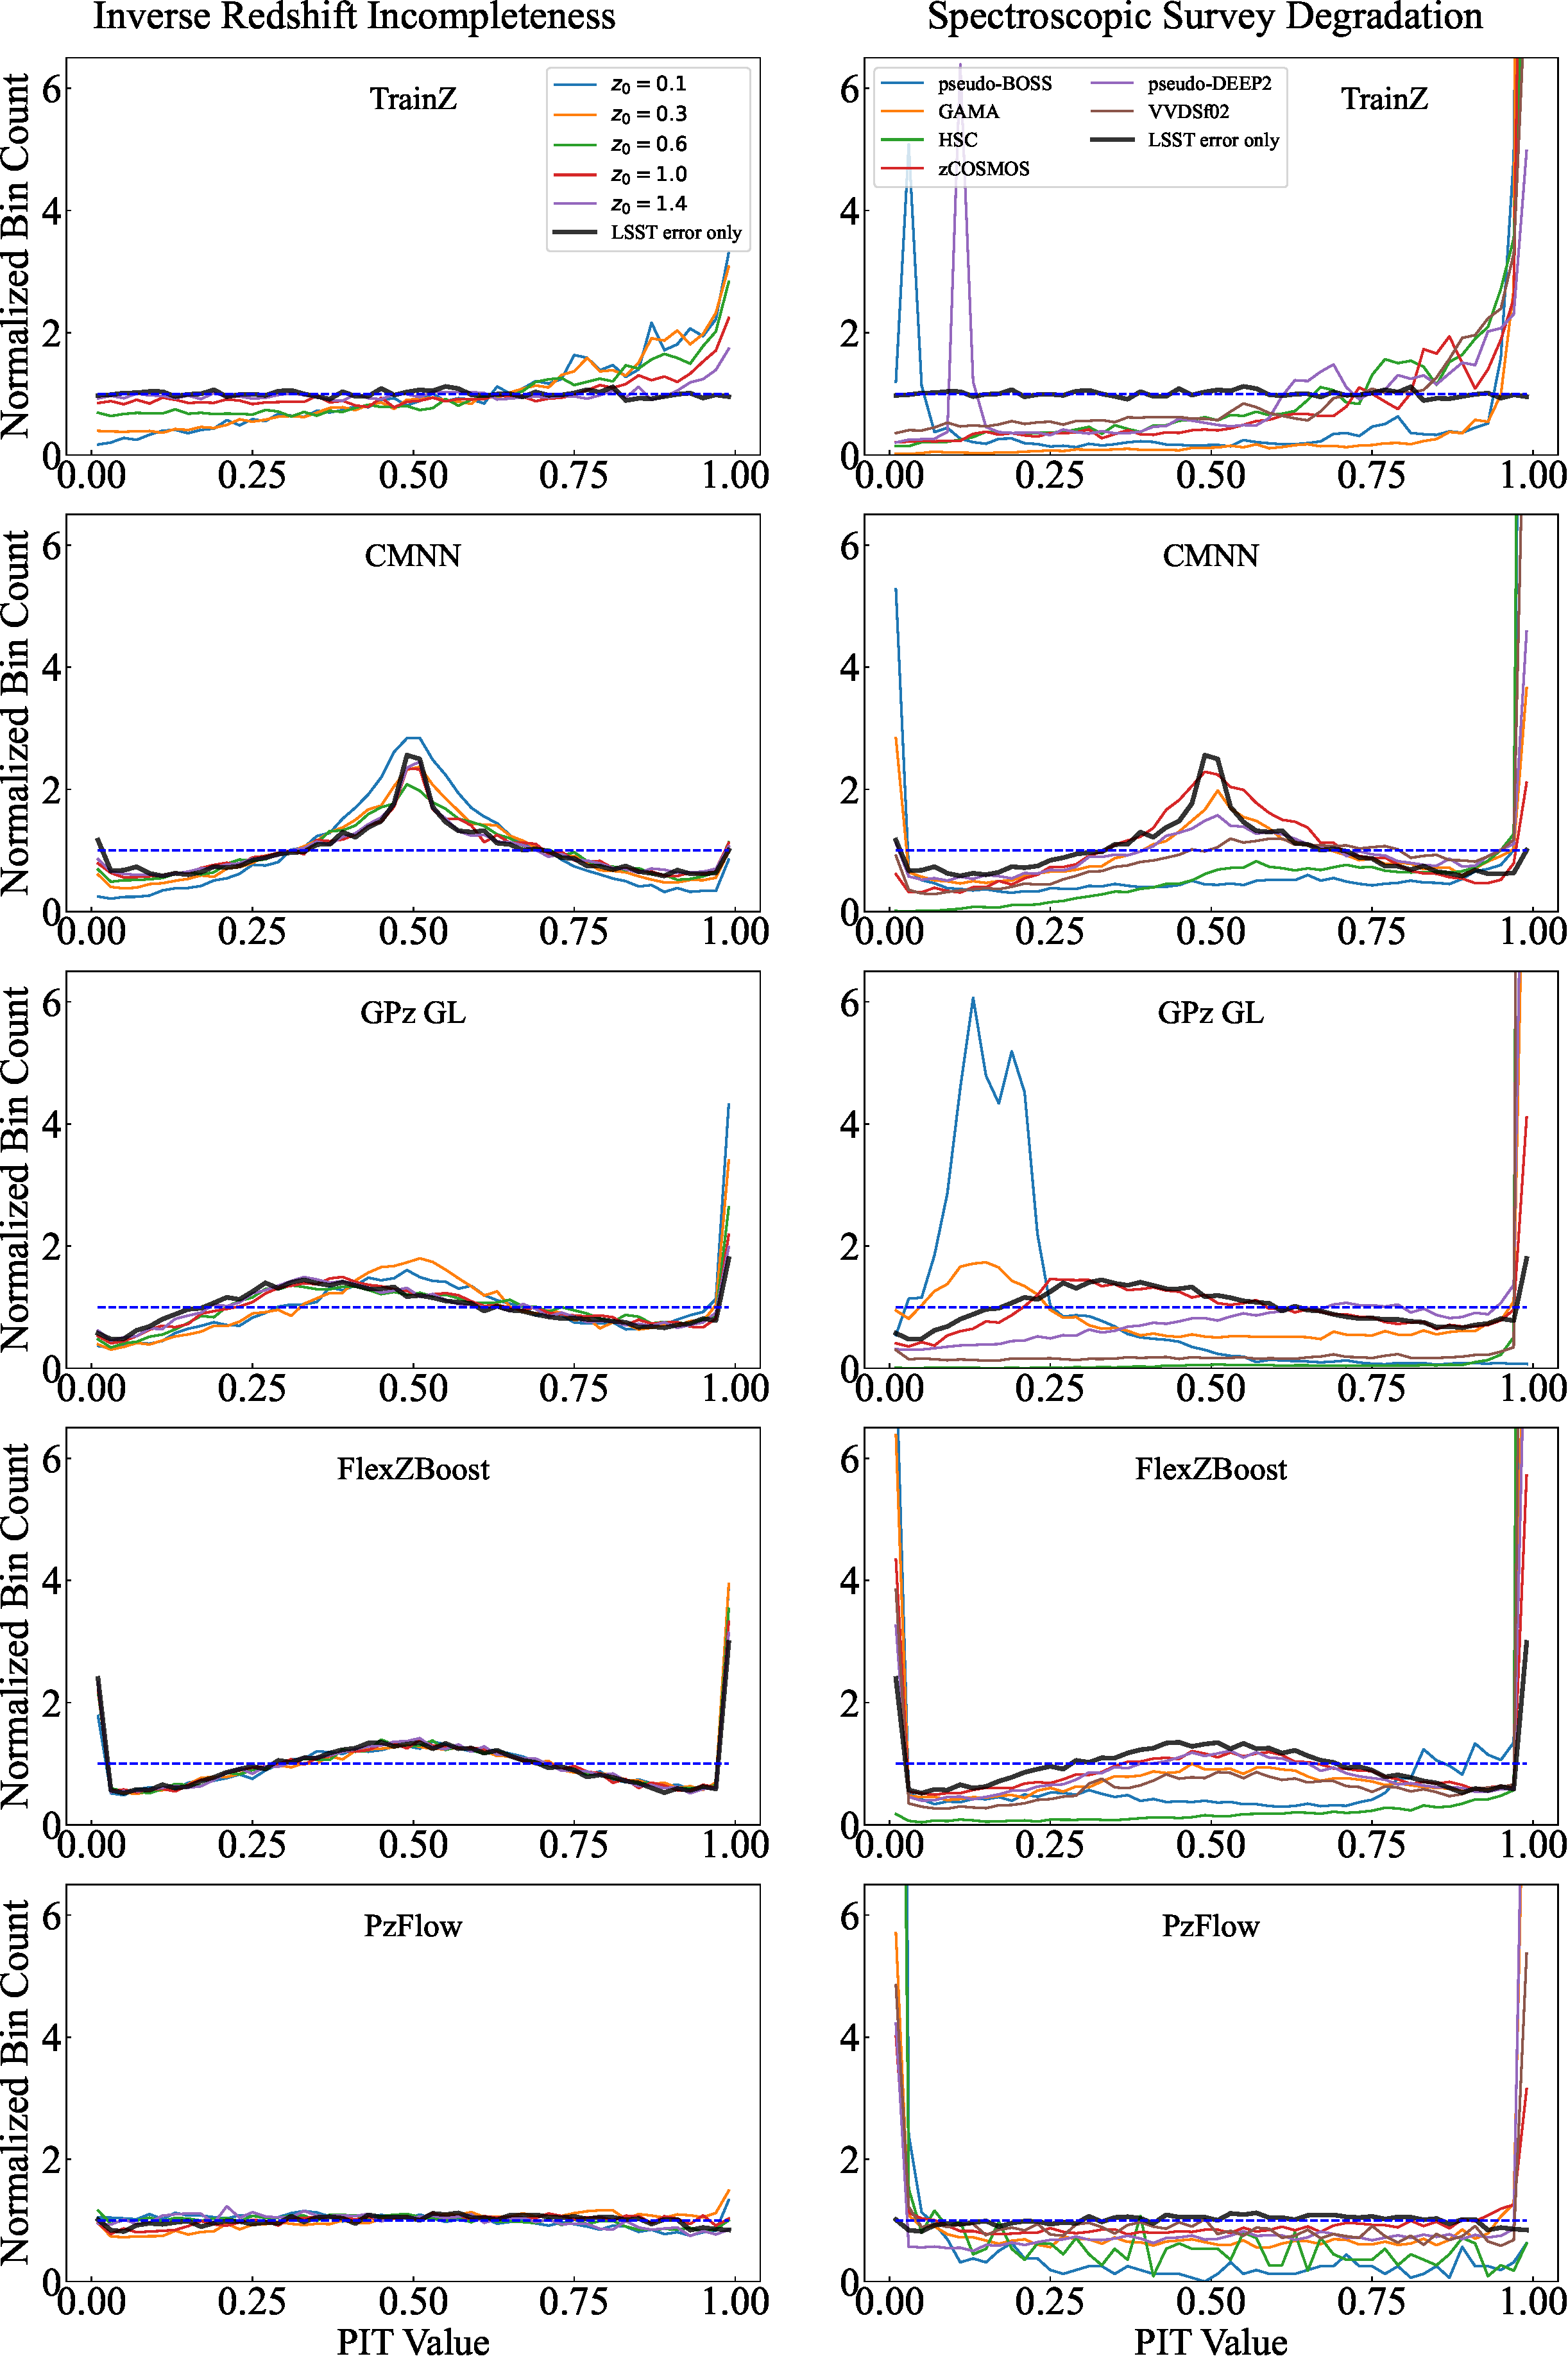
\includegraphics[width=0.7\textwidth]{PIT_lin.pdf}
  \caption{Probability integral transform distributions for inverse redshift incompleteness (left) and spectroscopic survey degradation (right). 
  A uniform distribution (ideal) is shown as a dashed line. We observe that each photo-$z$ estimator (shown in separate rows) has a distinctive and identifiable PIT shape. Shifts in this shape as degradation conditions are varied are more noticeable for Gaussian estimators than for \texttt{FlexZBoost} or \texttt{PzFlow}, though all experience a marked increase in side spike height under severe degradation, as expected. %\rachel{Once this is in review I'd like to work on making the legends easier to read, and on displaying the TrainZ label in the top row.}
  %\aim{Also the axis ticks/numbers can be omitted by squishing the panels closer.}
  }
  \label{fig:pit} 
\end{figure*}

\subsubsection{PIT}

In \citeDCt, the PIT and metrics thereof provided the most striking demonstration of the necessity of experimental controls like \texttt{TrainZ}, which consistently outperformed other estimation algorithms by the PIT under ideal conditions. As seen in the top left panel of Figure~\ref{fig:pit}, under biased training conditions \texttt{TrainZ}'s PIT curve is markedly shifted towards higher values. Thus in the presence of incomplete training data, \texttt{TrainZ} is no longer as useful as a control designed to optimize the PIT statistic. 
%\aim{Describe how TrainZ looks by the PIT under imperfect conditions.
%(This has never been done before and is a big deal for understanding the utility of this control case vs. the need for additional controls that tell us if our experiments overall are testing what we care about.)}

%\aim{The rest of this subsubsection also reads like it's a competition between estimators so should be reframed to highlight how the curves for a given estimator change, thus defining the kinds of behavior of the PIT we can anticipate with real imperfect training sets.
%(This is a very nice place to point out the qualitiatively different sensitivities of the gaussian estimators as opposed to the more flexible ones.)}

At all levels of degradation, \texttt{CMNN} (row 2) exhibits a clear middle bump, indicating that a disproportionate amount of its output $p(z)$ distributions are wider than the truth $p(z)$. 
%\rachel{could we say `wider than the truth $p(z)$' since it's a comparative metric?}\alice{Yes definitely!}
The bump becomes more pronounced as degradation becomes more severe, without shifting to the left or the right. This again indicates that the primary effect of increasing the inverse redshift degradation on \texttt{CMNN} outputs is increased standard deviation. 

The \texttt{GPz} PIT distributions in the left column exhibit both a middle bump and a right side spike, indicating a variety of distribution shapes in its outputs. The right spike implies a large fraction of underestimated distributions, while the middle bump again indicates an excess of distributions that are wider than the truth $p(z)$. As $z_0$ is increased and degradation becomes less severe, the right side spike decreases. This makes sense: since higher redshift data are becoming more complete as $z_0$ increases, the algorithm is less likely to underestimate the redshift. However, it is interesting to note the lack of any left spike; this indicates that under inverse redshift incompleteness, \texttt{GPz} produces virtually no catastrophically high outliers compared to low ones. Decreasing $z_0$ also shifts the middle bump downwards from $0.5$, indicating that broad, slightly under-estimated distributions may be common under idealized training conditions. We note also that for $z_0 \gtrsim 0.6$, little further shift in distributions is observed, again indicating that increasing $z_0$ beyond this approximate value yields diminishing returns on photo-$z$ estimation improvement.

\texttt{FlexZBoost} and \texttt{PzFlow} exhibit  remarkably robust PIT behavior for a variety of levels of inverse redshift incompleteness; decreasing $z_0$ has hardly any affect on the PIT distribution shape for either estimator. \refresponse{This example illustrates that the PIT's utility as a diagnostic for redshift incompleteness depends on the photometric \refresponsetwo{redshift} algorithm, and the PIT needs to be used alongside other, complementary metrics.} \texttt{FlexZBoost} exhibits pronounced spikes on both sides, as well as a modest middle bump. The presence of spikes on both sides indicates that narrow, slightly offset distributions are common for \texttt{FlexZBoost}. The middle bump implies that diffuse distributions, or potentially distributions that are bimodal about the truth, are also prevalent. \texttt{PzFlow}'s PIT distribution is remarkably featureless, closely approaching a uniform distribution in all cases, with only minor deviations as degradation worsens. 

As \texttt{GPz} and \texttt{CMNN} are both restricted to Gaussian output distributions, the effects of degraded data on their outputs will be qualitatively quite different than in the cases of \texttt{FlexZBoost} and \texttt{PzFlow}. In \texttt{GPz} and \texttt{CMNN} outputs, there are only two tuneable output distribution parameters: mean and standard deviation. The PIT exposes how these are influenced effectively: lack of horizontal shifts in the \texttt{CMNN} PIT distribution, yet continuous increase in middle bump height as degradation worsens, indicates a trend in widening standard deviations with little shift in means, whereas with \texttt{GPz}, change in side spike size as well as shifts in the overall distribution likely indicate a combination of the two. 

%\aim{And notably \cmnn and \gpz don't even share the same trends of severity, like \gpz is differently affected by low pivot redshifts but once they're higher than around 0.5 it doesn't get worse between those more severe cases, while with \cmnn we can see the trend of deviation for all values of pivot redshift, which is also true for the control case; it's definitely interesting to see that there are possibilities between ``totally insensitive to any redshift incompleteness" and ``gets worse as redshift incompleteness gets more severe."} 

\begin{figure*}
  \centering
  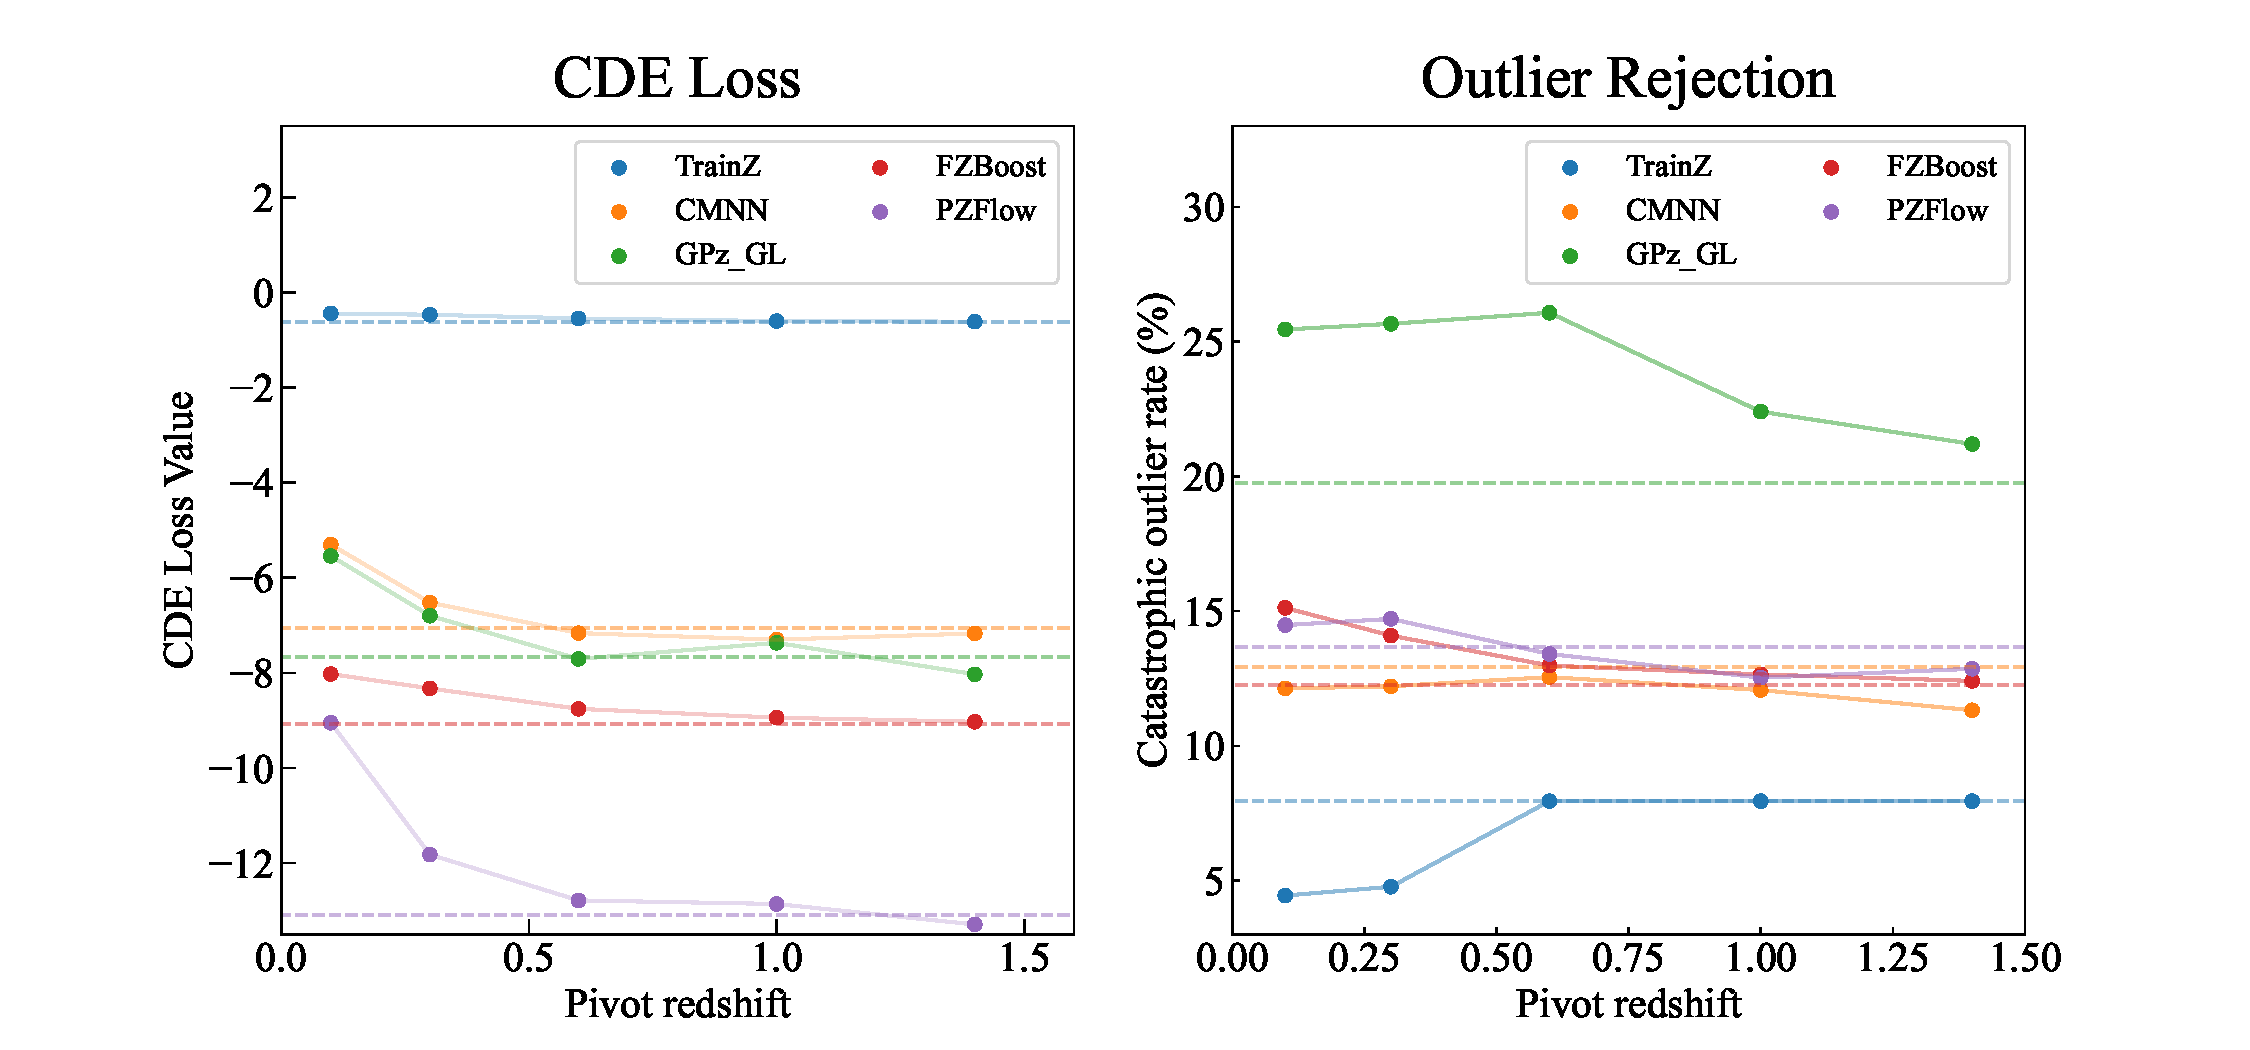
\includegraphics[width=0.95\textwidth]{Invz_CDE_OR.pdf}
  \caption{Plots of CDE loss values (left) and catastrophic outlier rates (right) as functions of the inverse redshift incompleteness pivot parameter, shown as solid lines. 
  Values for each estimator calculated under our control conditions (no inverse redshift incompleteness) are shown as dashed lines. We note that the CDE loss typically decreases as $z_0$ is increased, though we observe that the metric is far more sensitive to the estimator used than to the training set degradation. The catastrophic outlier rate decreases with increasing $z_0$ in some cases, but we see that this statistic is easily biased by scatter in point estimates, as the control estimator \texttt{TrainZ} appears to have done well.}
  \label{fig:invz CDE_OR} 
\end{figure*}

\subsubsection{CDE Loss}

The left panel of Figure~\ref{fig:invz CDE_OR} illustrates how the severity of inverse redshift incompleteness degradation affects the CDE loss metric. From examining the blue curve, we see that \texttt{TrainZ} has very weak evolution in the CDE loss as $z_0$ changes. Fortunately, the \texttt{TrainZ} CDE loss values are much higher (i.e., worse) than those for our non-control estimators, indicating that this statistic reflects galaxy-by-galaxy accuracy reasonably well. 

Results for \texttt{CMNN} and \texttt{GPz} (orange and green curves) are very similar to each other, with notable improvements as $z_0$ is increased, up to $z_0 \sim 0.6$. Though the trend is less pronounced, \texttt{FlexZBoost} exhibits mild improvements as $z_0$ increases. For lower values of $z_0$, \texttt{PzFlow} improvements are quite significant for increasing $z_0$. Though all non-control estimators exhibit some level of improvement in this statistic as degradation severity is decreased, results appear largely unaffected as $z_0$ is increased beyond $\sim$0.6 for all estimators. This suggests that increasing a theoretical pivot redshift beyond $z_0 \sim 0.6$ will result in minimal further improvements in the aspects of photo-$z$ estimation to which the CDE loss is sensitive. We also note that while the CDE loss is marginally sensitive to this form of training set degradation, it appears to be far more sensitive to the choice of estimator than to training set properties. 

\subsubsection{Outlier \revone{Rejection}{Identification}}

The right panel of Figure~\ref{fig:invz CDE_OR} shows trends in the catastrophic outlier rate as $z_0$ is increased for each of our photo-$z$ estimators. As discussed in Section~\ref{sec:outlier rejection}, this statistic is artificially low and not particularly meaningful for \texttt{TrainZ}. Our non-control algorithms provide more interesting results. \texttt{CMNN} and \texttt{PzFlow} show only weak trends here, as outlier rates fluctuate with respect to the baseline determined in the representative control case. For \texttt{FlexZBoost}, though the trend is slight, there is a clear decrease in outlier rate as $z_0$ is increased. 

As with its PIT and CDE loss, \texttt{GPz} seems to exhibit two distinctively different behaviors for $z_0\lesssim 0.6$ and $z_0 \gtrsim 0.6$. At low $z_0$, outlier rates are high, and approximately constant with $z_0$. However, there appears to be a decreasing trend in outlier rate as $z_0$ is increased past $0.6$. Unlike for the CDE loss, this statistic indicates that for \texttt{GPz}, there is continued improvement in performance as $z_0$ continues to increase past $0.6$. 
% \aim{This is a good place to contrast \gpz with the others \textemdash we can see the same unexpected behavior as in the PIT, where it treats $z_{0} > 0.5$ and $z_{0} < 0.5$ differently, to the extent that it's getting into the realm of the control case where this metric doesn't really tell us what we care about. }
% Also, you can make the general statement that the others have higher rates at low pivot redshift and only improve slightly with higher pivot redshift.
% (And repeating general statements like this in the captions is also good.)}

% \aim{Agreed!
% It's always hard to know where to put the kinds of things in the next paragraph\dots
% Maybe @Rachel has some thoughts on it?}
%\newline

\subsubsection{Summary of metric results for inverse redshift incompleteness}

Overall, the effects of inverse redshift incompleteness degradation are small in comparison with the effects of spectroscopic survey degradation across all algorithms (see Section~\ref{sec:spec}). 
However, some metrics illustrate these small differences more effectively than others, and different photo-$z$ algorithms have differing sensitivity modes. The KS test, RMSE, and KLD reflect little in terms of the difference in performance across different $z_0$ cases, yet provide a helpful picture of overall estimation accuracy. The CvM test exposes small differences in performance across $z_0$ cases in the Gaussian photo-$z$ estimators, yet shows very little change for others. The PIT provides valuable insights into shifts in distribution shapes, particularly for Gaussian estimators, and illustrates two different behaviors for \texttt{GPz} in cases where $z_0 \lesssim 0.6$ and $z_0 \gtrsim 0.6$. The CDE loss illustrates clear performance improvement for all estimators up to $z_0 \sim 0.6$, yet shows little further improvement as $z_0$ continues to increase. Outlier rejection results are scattered for \texttt{CMNN} and \texttt{PzFlow}, while showing clear improvement for \texttt{FlexZBoost} as $z_0$ increases, and also capturing \texttt{GPz}'s differing behavior for $z_0 < 0.6$ and $z_0 > 0.6$ 


% \aim{This is another place to refocus on metrics rather than algorithm comparisons.}



\subsection{Spectroscopic Survey Degradation Effects}
\label{sec:spec}

As anticipated, we find that the more varied and severe forms of incompleteness introduced with spectroscopic survey degradation have more significant effects on photo-$z$ estimation results than the toy form of degradation created by the inverse redshift incompleteness degrader.  
%
We naturally expect that more severe degradation should correspond to worse photo-$z$ performance that would be reflected in our metrics. As pseudo-BOSS is catastrophically incomplete, we expect it to fail more catastrophically than all other training sets, and produce both inaccurate and imprecise results. We  expect similarly poor performance from GAMA, though perhaps to a lesser degree as it is larger, and potentially biased performance under zCOSMOS and pseudo-DEEP2 degradation, placing precise estimates preferentially in the regions of redshift-magnitude space they cover with low accuracy for uncovered regions. 
%\rachel{I was wondering what distinction is meant by `very poor performance' versus `biased' - is one about precision and the other about accuracy?  I think we should use more specific adjectives in this paragraph.} 
As coverage is high under VVDSf02 and HSC degradation, we expect performance under these conditions to be both more accurate and more precise. 
We examine below the correlation between algorithmic performance across our various metrics and training set coverage of redshift-magnitude space and/or training set size.

\begin{figure*}
  \centering
  
\includegraphics[width=1.0\textwidth]{Spec_Dist-to-dist.pdf}
  \caption{Quantile plots of the \refresponse{logarithmic} CvM, KS, RMSE,  KLD, and Wasserstein Distance statistics (columns) for each photo-$z$ estimation algorithm (rows), under each case of spectroscopic survey degradation (colors indicated in legend). Lines \refresponse{curving to the bottom right} indicate a larger proportion of high statistic values, and thus poorer performance. \refresponse{Galaxies with invalid \texttt{PzFlow} estimates are discarded to normalize the curves to unity.}  We see significant differentiation between the curves for \refresponse{different degraders for all metrics except for the KS test, and the performance patterns under degradation are mostly consistent across different photo-$z$ algorithms. We note that the BOSS and GAMA degraders result in particularly bad photo-$z$s, which is consistent with our expectation since these degraders only select bright training galaxies with a particular color cut. }
  % \aim{Let's order these by number of galaxies for all the survey-specific cases.}
  }
  \label{fig:spec d2d} 
\end{figure*}

\subsubsection{CvM, KS, RMSE, KLD, W.\ Distance}

% \alice{@alex if you could take a look at this part and leave any specific feedback you have that would be great!}

Figure~\ref{fig:spec d2d} summarizes the distribution-to-distribution statistics for each spectroscopic degrader and photo-$z$ estimator. 
In contrast with the inverse redshift incompleteness degradation, we see significant variation between the different degraders in practically every case, and the metrics have differing sensitivity to the different degraders' impact on each estimator. 
% A common trend is that a subset of (but not all of) our statistics reflect poor performance in the BOSS and GAMA cases. 
% In some cases, performance with the zCOSMOS degrader is also particularly poor. 

\texttt{TrainZ} performance (shown in row 1) seems to be strongly correlated with the number of galaxies in its training set (provided in Figure~\ref{fig:spec CDE plot} \cwr{and Table}~\ref{tab:spec rej}) and affected minimally by training set coverage, as indicated by \refresponse{similar} performance in the pseudo-DEEP2 and VVDSf02 cases \refresponse{as for} the HSC case in several metrics. 
The CvM and KLD show this particularly clearly. 
The RMSE provides no means of differentiating between different forms of incompleteness for \texttt{TrainZ}, while the KS test and Wasserstein Distance show little variation except in the cases of pseudo-BOSS and \refresponse{GAMA}, where large fractions of redshift-magnitude space are missing from the training data. 


\texttt{CMNN} results are provided in row 2. 
We see that all  metrics \refresponse{except for the KS test} can discriminate between the two catastrophically incomplete training sets (with the pseudo-BOSS and GAMA degraders) and the other four. 
Low CvM values for these two cases are likely explained by wide output distributions, i.e.~the effect illustrated in Figure~\ref{fig:stdev fx}. 
There is \refresponse{less} variation in photo-$z$ performance when applying the pseudo-DEEP2, HSC, VVDSf02, and zCOSMOS degraders as quantified with any of the other metrics, though \refresponse{all but the KS test reveal some differences between the degraders}. 
The relatively minor effect on performance in the zCOSMOS case indicates that \texttt{CMNN} is successful at interpolating to regions of redshift-magnitude space that are only minimally covered by training data. 

\texttt{GPz} results are provided in row 3. 
The distributions of metric values shift significantly across our training sets, though the RMSE is \refresponse{the least sensitive of the metrics shown}. 
The other statistics, however, capture well the surprisingly poor performance of \texttt{GPz} on the zCOSMOS training set. 
Notably, the Wasserstein Distance captures a clear correlation with average training set coverage, as seen by examining the left-to-right ordering of the curves. 
As expected, estimation was largely unsuccessful on the pseudo-BOSS and GAMA cases, as shown by the significant deviation of the blue and green curves from the rest, which is particularly obvious in the KLD and Wasserstein distance.
%\aim{Which metrics showed the previous statement?}
It may be surprising how little the two cases differ from each other, but in fact the vast majority of estimates for both cases are what we may consider to be `failures' (see Section~\ref{sec:failure rates}): 
when a test galaxy is inadequately represented in training data, \texttt{GPz} returns so large a variance that the distribution is broad enough to appear to be a nearly flat line at $p(z) = 0$ for all $z$.
%\aim{Do you mean $p(z)=0\forall z$ or $z=0$?}
Thus the localized spike for pseudo-BOSS and GAMA distributions present across most of our statistics corresponds to the value each takes on in the case of a ``flat'' distribution compared with a narrow, unimodal distribution. 
The fact that zCOSMOS has under-performed or performed similarly when compared with these cases indicates that a significant fraction of its outputs are truly incorrect estimates not flagged by the algorithm as failures. 
This demonstrates the need for multiple metrics, specifically the interpretation of outlier/failure rates in addition to the distribution-to-distribution metrics.

\texttt{FlexZBoost} results are presented in row 4. 
Again results are split between pseudo-BOSS and GAMA versus the other four surveys, though the two catastrophically incomplete cases differ significantly from each other in several metrics. 
Perhaps surprisingly, GAMA estimation appears less successful than pseudo-BOSS estimation according to most metrics. GAMA curves (green) are shifted notably to the right in the \refresponse{CvM}, KS test, KLD, and Wasserstein distance when compared with pseudo-BOSS curves, indicating a larger proportion of high statistic values.
%\aim{Tell the reader which metrics show this and how you know it.}
Though \texttt{FlexZBoost} does not have a well-defined notion of failure, distributions corresponding to galaxies that are not well-represented in training data are often very broad or multi-modal, appropriately indicating uncertainty. 
The vast majority of pseudo-BOSS outputs are such distributions, whereas a larger proportion of GAMA outputs are likely truly inaccurate estimations, similar to the zCOSMOS case with \texttt{GPz}. 
\texttt{FlexZBoost} estimates with the zCOSMOS degrader appear mildly worse than those for HSC, VVDSf02, or pseudo-DEEP2 degraders, particularly in the Wasserstein Distance, though the difference is not extreme.  

Row 5 presents \texttt{PzFlow} results. \refresponse{As noted in the caption, galaxies with invalid \texttt{PzFlow} estimates are discarded so the curves normalize to unity.}
%Distributions of metric values appear starkly different than for all other estimators, as \texttt{PzFlow} fails to produce estimates for most test set galaxies insufficiently represented from training sets (see Section~\ref{sec:failure rates}). 
%Thus its sensitivity to training set coverage is readily evident, and we see a direct correlation between coverage percentage and the number of test set galaxies on which successful estimates are made. 
%HSC, with approximately 79$\%$ average coverage of the test set across all bands, is the only non-control training set for which an estimate was successfully made for all galaxies. 
%Despite a difference of only approximately 7.5$\%$ in average coverage between HSC and VVDSf02, far fewer galaxies had successful photo-$z$ estimates. 
%The greatest difference between the two surveys is their coverage in the $i$, $z$, and $y$ bands, indicating that these bands may play an important role in \texttt{PzFlow}'s estimation success.
It is worth noting a distinction between the results for pseudo-BOSS and GAMA: 
\texttt{PzFlow} produced similar numbers of estimates for each case, but with much higher accuracy for the GAMA training set. 
The increase from the $\sim$$10\%$ average coverage in pseudo-BOSS to the $\sim$$25\%$ \refresponse{coverage of GAMA %did little to improve the failure rate, but 
significantly improved the accuracy}. This is clearly visible in the leftward shifts of the GAMA curve in the CvM and RMSE results shown in Row 5 of Figure \ref{fig:spec d2d}, but is made the most obvious by examining the CDE loss (see Figure \ref{fig:spec CDE plot}). 
%\aim{State what in the figure indicates the previous statement.}
%In contrast, the $\sim$$35\%$ average coverage with zCOSMOS significantly decreased the failure rate, though it still remained high. 

Across all estimators, the \refresponse{CvM}, KLD and Wasserstein Distance consistently provided an informative \refresponse{view on how algorithm performance depends on the training set incompleteness}, while the RMSE \refresponse{and KS test show little (or inconsistent)} variation across different degrees of training set degradation, except in catastrophically poor cases that are unlikely to occur in realistic data. 
Due to its sensitivity to distribution tails, the CvM test at times distinguishes differences in performance not captured by other statistics, but as it is easily biased, % \aim{What is meant by this? Just that it's easily thrown off?}, 
it does not often provide an accurate picture of photo-$z$ estimator success on its own. 
For a few of the examined estimators, the KS test is \refresponse{relatively insensitive to training set incompleteness except in truly catastrophic cases, but as noted previously, it has the advantage of being} sensitive to shifts in distribution shape in the opposite way from the CvM and KLD tests (see Figure~\ref{fig:stdev fx}). 

%\aim{Nice work reframing the focus away from comparing estimators to one another!
%Overall, this section would nonetheless be strengthened by saying which metric(s) support(s) each statement of sensitivity of an estimator to a degrader;
%you've spent a lot more time looking at Figure~\ref{fig:spec d2d} than the readers will have, so tell them what you're seeing in which curve to make you think there is or is not sensitivity.}

\subsubsection{PIT}


Comparing the left and right columns of Figure~\ref{fig:pit}, we see that overall distribution shapes and trends in the PIT curves for the spectroscopic degradation cases are similar to those in the inverse redshift incompleteness cases, with the exception of the catastrophically incomplete pseudo-BOSS and GAMA training sets, and in the case of \texttt{GPz}, zCOSMOS as well. Side spikes become more prominent in the presence of severe degradation for all estimators (note the logarithmic scaling of the vertical axis in the right column of Figure~\ref{fig:pit}), though the PIT helpfully captures whether algorithms preferentially \cwr{produce outliers to low versus high redshift} when we compare the relative sizes of the left and right size spikes. For example, similarly-sized left and right side spikes for \texttt{CMNN}, \texttt{FlexZBoost}, and \texttt{PzFlow} indicate that catastrophically high and low outliers are roughly equally common from these alorithms, whereas the lack of a left side spike for \texttt{TrainZ} and \texttt{GPz} indicates that these algorithms are prone to under-estimation under these degradation conditions. 
This is an example of the clear illustration of trends in the specific way(s) in which algorithms can be inaccurate that the PIT provides, which is not provided by other metrics. 
%\rachel{I think the commentary on the side spikes reads more like an evaluation of \texttt{TrainZ} and \texttt{GPz} rather than commentary on how informative (or not) the PIT is, so I would suggest reframing that.}
%\aim{Agreed.}


\subsubsection{CDE Loss}

\begin{figure*}
  \centering
  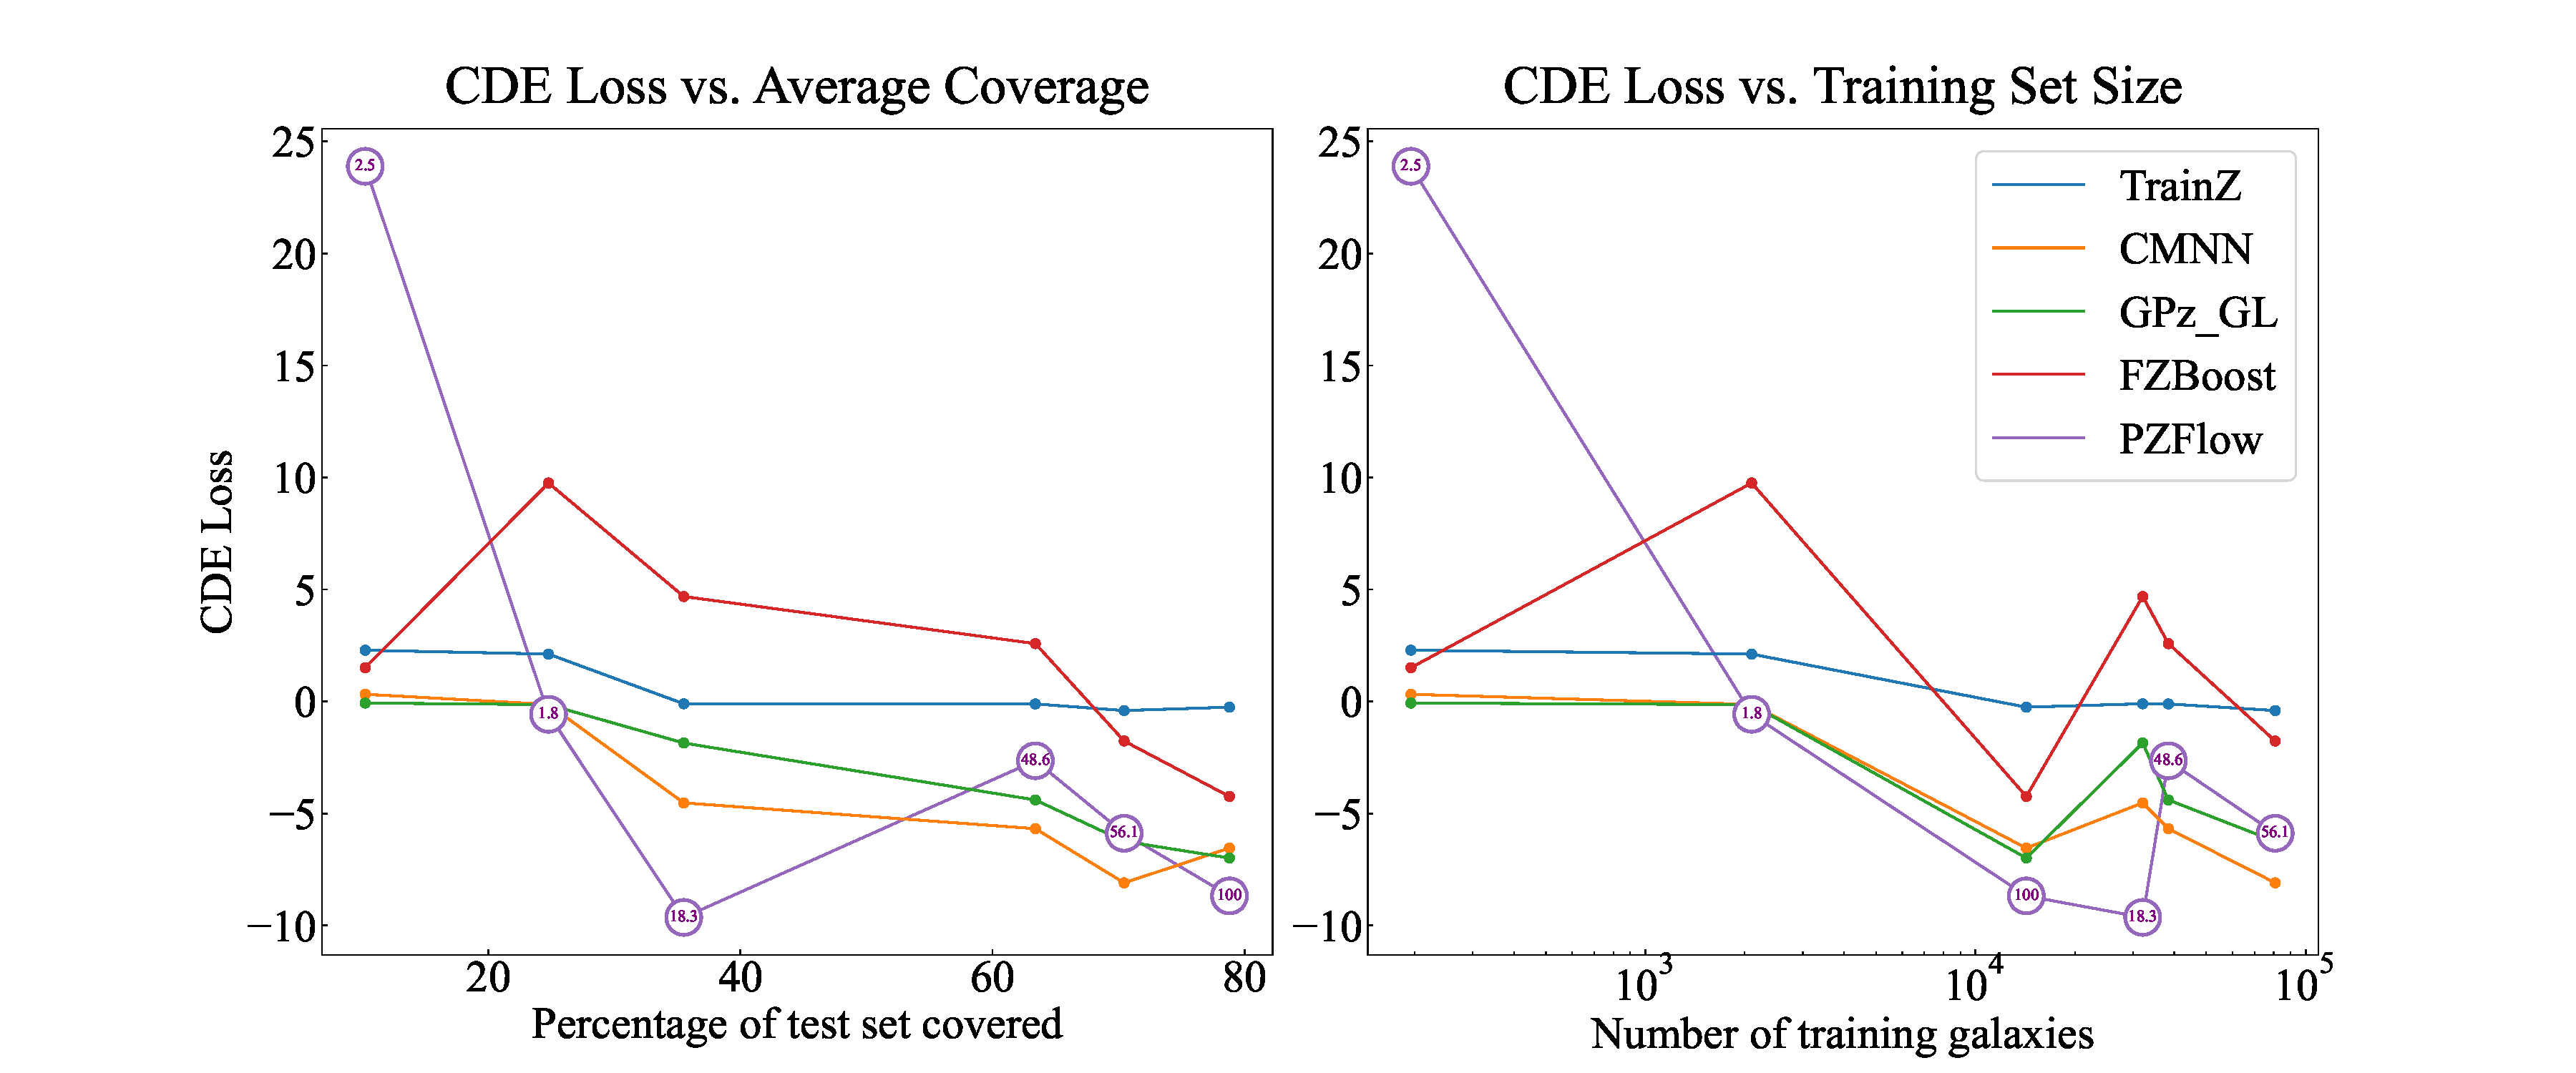
\includegraphics[width=0.9\textwidth]{Spec_CDE.pdf}
  \caption{CDE loss plotted both as a function of training set coverage of the test set (left) and training set size (right). For most estimators, we see a relatively smooth downward trend in CDE loss as coverage increases, whereas we see much more scatter when considering training set size alone. 
  %\rachel{I see similar trends in both.  Has the figure changed and does this need to be updated?} 
  Since \texttt{PzFlow} has failed to produce an estimate for large fractions of most of our training sets, this \texttt{PzFlow} data only accounts for the galaxies on which estimation successfully occurred. We have included the \texttt{PzFlow} success rate for each training set in the center of each \texttt{PzFlow} data point. } 


\label{fig:spec CDE plot} 
\end{figure*}


Examining Figure~\ref{fig:spec CDE plot}, we see that many results shown in Figure~\ref{fig:spec d2d} are corroborated. 
Examining the left panel of Figure~\ref{fig:spec CDE plot}, we see a clear anti-correlation between training set coverage and CDE loss value for \texttt{CMNN} and \texttt{GPz}. \texttt{TrainZ} shows very weak evolution as training set coverage increases past around $25\%$. With the surprising exception of the pseudo-BOSS case, \texttt{FlexZBoost} also shows a clear decrease in CDE loss as coverage is increased. The trend in \texttt{PzFlow} results is not as clear, though note that only galaxies for which successful estimation was performed contribute to this statistic. Nevertheless, with the exception of the GAMA case, a monotonically decreasing trend in CDE loss appears as coverage is increased. The surprisingly low zCOSMOS value is likely due to high accuracy in the smaller number of estimates made, but does not reflect the failure rate of over $80\%$. 

Examining both coverage and training set size, performance is obviously poor in our catastrophically incomplete cases. Though there is a downward trend as both coverage and training set size are increased, the coverage trend is much clearer, showing monotonic or nearly monotonic decreases in all but the \texttt{PzFlow} case. Though there is also a decreasing trend in CDE loss as we increase training set size, the scatter is much more significant. 
%\rachel{I see monotonic decreases for CMNN, PZFlow, and net decrease with a bit of scatter for FZBoost and GPz.  To me it seems like the trend is there, albeit with more scatter than the trend with coverage.} 
All non-control algorithms show the most significant scatter among the larger training sets, indicating that training set size alone is not an necessarily an accurate indicator of potential performance success without also considering coverage of redshift-magnitude space.

Finally we also note that, similar to the inverse redshift incompleteness case, in many instances differences between estimators are exposed more starkly by this metric than differences across training sets. While this metric may be successful at distinguishing estimators from one another, it is not as indicative of the effects of training set imperfections as some others examined here. 

\subsubsection{Outlier Rejection}

\begin{table*}
\begin{center}
\begin{tabular}{||c c c c c c||} 
 \hline
 Degradation Type: & \texttt{TrainZ} & \texttt{CMNN} & \texttt{GPz} GL & \texttt{FlexZBoost} & \texttt{PzFlow}\\ [0.5ex] 
 \hline\hline
 pseudo-BOSS (195 galaxies): & 7.133 & 10.19 & 25.45 & 15.97  & 2.644 $\&$ 97.45 $\rightarrow$ 97.51\\
 \hline
 GAMA (2,099 galaxies): & 4.410 & 3.778 & 26.07 &  3.049 & 0.535 $\&$ 98.21 $\rightarrow$ 98.22\\
 \hline
 HSC (14,253 galaxies): & 4.432 & 16.03 & 26.25 & 17.60 & 19.78 $\&$ 0.0 $\rightarrow$ 19.78\\  
 \hline
 zCOSMOS (32,089 galaxies): & 5.504 & 25.97 & 0.0 & 24.57 & 16.05 $\&$ 81.67 $\rightarrow$ 84.61\\  
 \hline
 pseudo-DEEP2 (38,385 galaxies): & 7.027 & 15.43 & 25.66 & 15.68 & 41.78 $\&$ 51.38 $\rightarrow$ 71.61\\
 \hline
 VVDSf02 (80,845 galaxies): & 8.186 & 21.17 & 39.62 & 20.68 & 37.88 $\&$ 43.86 $\rightarrow$ 65.13\\
 \hline\hline
 LSST Error Model only (30,953 galaxies): & 7.949 & 12.91 & 19.75 & 12.27 & 13.67 $\&$ 0.0 $\rightarrow$ 13.67\\ [1ex] 
 \hline
\end{tabular}
\caption{Table showing percentage of estimates considered catastrophic outliers via outlier rejection for estimators trained on spectroscopic survey degraded data. For \texttt{PzFlow}, two numbers are shown: the first is the catastrophic outlier rate among successful estimates, the second is the percentage of the test data for which no estimate was made. The third number is the percentage of the test set that either produced a catastrophic outlier or a failed estimation. It is clear that outlier rate does not display a reliable correlation with the variation of training set perfection, either as size or coverage are changed. }
%\aim{``It is clear that the outlier rate does not display a correlation with the variation of training set perfection\dots"}}
\label{tab:spec rej} 
\end{center}
\end{table*}

As discussed in Section~\ref{sec:outlier rejection}, the outlier rejection metric is easily biased low by large standard deviations in output point estimates. Examining \refresponse{Table}~\ref{tab:spec rej}, we do see this reflected in our results. The outlier rejection metric produces low values for several cases in which we would expect poor performance, due to very large scatter in the results.
%\rachel{By `indeed', do you mean this is evidence of the bias referred to previously?(low = good and we expected poor performance)} 
\texttt{TrainZ} values differ little from those in the inverse redshift incompleteness case, as we expect. This effect also explains some surprisingly low pseudo-BOSS and GAMA results, and the `0.0' for \texttt{GPz}'s zCOSMOS case. 
However, we do not simply see an inverse correlation with outlier rate and performance either, as in some cases this metric appears high where we would expect it to be low, or does indeed perform as expected. 
Due to the multiple features of the distributions of outputs that affect this statistic, we do not find a simple relationship between outlier rate calculated via this method and either training set coverage or size. In cases where the distribution of mode estimates is supposed {\em a priori} to be a narrow cluster about the diagonal, this statistic provides an informative description of catastrophic outlier rate. However, in cases of poor estimation, this statistic is easily biased towards being unrealistically low, and therefore is not a reliable indicator of performance in such cases. 

\subsection{Failure Rates}
\label{sec:failure rates}

% \alice{@alex what thoughts do you have on this part?}
% \aim{It's great! 
% I added a couple sentences to clarify the line of reasoning up front.}
If an algorithm is tested on data that it judges to be far enough from its training set as to make its predictions unreliable, it would be preferable for it to fail to perform any estimation or return a distribution that adequately indicates this uncertainty, as opposed to taking a wild guess. 
Indicators of unreliability are in a sense a metric that an algorithm can deliver to users, and different algorithms do this to varying degrees.
Here we discuss some of the ways such flags manifest among the algorithms we tested and how effective we found those indicators to be.


As seen in the rightmost column of \cwr{Table}~\ref{tab:spec rej}, \texttt{PzFlow} rarely produces estimates for data that is not well-represented in its training set, with the exception of small gaps. 
This would make \texttt{PzFlow} an ideal choice in situations where accuracy is prioritized over completeness of photo-$z$ estimation.

For the other examined algorithms, quantifying a `failure rate' is not as straightforward, and would necessitate further work. With \texttt{GPz} for example, a certain mean or standard deviation could be used to establish a cutoff above (or below) which an estimate is considered a `failure', as \texttt{GPz} returns distributions with identifiably %\alice{spelling??}\rachel{it's fine} 
extreme parameters under poor training set representation. This leaves the judgment of success somewhat up to the user, though it may necessitate further post-estimation data processing. 

\texttt{FlexZBoost}'s notion of `failure' seems nebulous, though distribution multimodality may serve as a useful metric in cases of extremely poor training. Severely multimodal distributions could be chosen to constitute failures, but again this requires additional data examination after estimation is complete, and identifying multimodal distributions is not as easily implementable as a mean or standard deviation cutoff in the case of \texttt{GPz}. Given that even under GAMA training set conditions, such multimodal distributions were rare, \texttt{FlexZBoost} is ineffective at identifying when it cannot make an accurate estimate.

\texttt{CMNN} has little to no notion of estimation ``failures'' in its outputs: most distributions have passably reasonable parameters, so `failed' estimations cannot be identified as those with means of $\sim$$200$ or standard deviations of $\sim$$50$ for example, as in the case of \texttt{GPz}. This hinders accuracy under poor training set conditions, without making this obvious to the user. 

\texttt{TrainZ}, by definition, never reports a notion of unreliability. 


\section{Conclusion}
\label{sec:conclusion}


\refresponse{Incompleteness and non-representativeness of spectroscopic training sets are common problems for photometric redshift estimation with deep imaging surveys.  In this work, we have investigated how a variety of metrics commonly used to quantify the performance of photometric redshift algorithms in RAIL react to (and can serve as diagnostics of) imperfections in spectroscopic training samples.  We considered the case of inverse redshift incompleteness, and non-representativeness associated with a variety of spectroscopic surveys.  The photo-$z$ performance metrics were applied to multiple different photo-$z$ algorithms -- without attempting to optimize or fine-tune their hyper-parameters -- as a demonstration of how these metrics react to training set imperfections.}

It is clear from our work that spectroscopic non-representativity effects have more severe consequences for \refresponse{photo-$z$} estimation accuracy than incompleteness effects, regardless of the algorithm being used. We conclude that, as expected, inverse redshift incompleteness degradation alone does not realistically approximate the complexity of real training data.
We also clearly demonstrate the need for multiple metrics in order to make a complete and accurate assessment of an algorithm's performance. {Here we recapitulate our conclusions for individual metrics:}

\begin{itemize}
\item The RMSE is affected comparatively little by the kinds of degradation we have examined. Only in the cases of catastrophically incomplete spectroscopic survey degradation is it significantly affected. It provides little information on algorithm performance in comparison with the other metrics examined here. As is examined in \citet{malz_approximating_2018}, the RMSE lacks sensitivity to distribution tails, and horizontal shifts of output distributions (which significantly affect tails) are very common under our degradation conditions. Thus the RMSE misses much of the changes in estimation behavior. 
\item The CvM test is quite sensitive to changes in training data, likely due to its high sensitivity to distribution tails. However, it is heavily biased by distribution shape, and often gives an inaccurate representation of performance. In several cases CvM values are (misleadingly) lower for instances of poor performance (such as when training with the pseudo-BOSS/GAMA surveys), and high where we know estimation is more accurate. It is an effective tool for picking up small variation in output distributions as training data are changed, but does not reflect estimator accuracy well on its own. 
\item Though the KS test is also susceptible to biases induced by distribution shape, we note that it may be informative when combined with other metrics, as it responds differently to systematic bias than either the CvM or KLD, as shown in Figure \ref{fig:stdev fx}. 
\item The KLD adequately \refresponse{reflects} differences in performance between spectroscopically degraded training sets. There is an obvious correlation between KLD value distributions and training set coverage, and we note that this statistic has also successfully identified some cases with high rates of inaccurate estimation. 
\item The Wasserstein Distance is also reliably representative of algorithm performance. It illustrates a clear correlation between training set coverage and performance for several algorithms, which is not shown as clearly by other metrics. 
\item The PIT reveals valuable information about distribution shapes not necessarily captured by other performance metrics, as it illustrates whether distributions are characteristically too wide (``middle bumps'') or too narrow (``side spikes''). %Combined with distribution-to-distribution statistics, the PIT provides a more complete picture of performance than either would alone. 
\item The CDE loss metric shows modest correlation with training set coverage for most estimators, and provides a ``single number evaluation'' of performance. Though it does not necessarily provide a reliable picture of performance in instances of high failure rates, it provides a concise assessment of performance and is quick to implement. However, it seems to be more sensitive to differences between algorithms than training set imperfections. 
\item While catastrophic outlier rate is a very helpful metric with which to assess algorithm performance, implementing it via outlier rejection produces varied results. In cases of very poor estimation, outlier rejection produces an artificially low outlier rate, thus giving an inaccurate picture of performance. We recommend using a different method to identify catastrophic outliers in such cases. However, in cases where estimation produces a relatively tight distribution of point estimates, outlier rejection can be a valuable technique for identifying catastrophic outliers. 
\end{itemize}

We also note that further work on the quantification of failed estimation with \texttt{CMNN} and \texttt{FlexZBoost} is necessary in order to make their results optimally useful. %\alice{more here?} \rachel{I would just add this:}  
This will be especially interesting in future work that considers estimation method optimization and different sample selections, which could be quite relevant to estimation failures.

\cwr{Future work could also employ these metrics in the context of statistical approaches to understand the impact of covariate shifts due to mismatches between training and testing sets, for example the stratified learning approach of \cite{https://doi.org/10.1002/sam.11643} and \cite{2025OJAp....8E..50M} that relies on analysis of subsets of the training and test sets prior to considering the full sample.}

%\alice{can I end this here? or should I have another short paragraph} \rachel{It's good to have something about the future outlook at the end of this section.  I've drafted something here; please see what you think --}

In this work, we have shown the strengths of various statistical metrics to quantify the performance of photo-$z$ algorithms in the context of relatively simple test cases: a handful of photo-$z$ algorithms with default parameter settings, and with a limited illustrative set of training set imperfections.  The outcomes demonstrated here can serve as the basis for future work that will be important to carry out before analysis of LSST data using photo-$z$.  For example, a more thorough method comparison while allowing for estimation method parameter tuning will be an essential exercise.  In this work, we considered 10-year LSST depth, but studies prior to early LSST analyses will need to consider more shallow and less homogeneous datasets such as those that will be acquired in the first year of the survey. Here we considered a \refresponse{fixed} test set, but in reality it will be useful to explore how sample selection might usefully be varied to accommodate the performance of photo-$z$ estimation algorithms.  It will also be important to consider the impact of blending of galaxy light profiles, which requires a study based on simulated or real imaging rather than the extragalactic catalogs used in this work.  \cwr{Finally, we note that the models for the extragalactic galaxy sample in \citet{2025MNRAS.544.3799O}, as used for this work, have continued to evolve after publication of that work, and tests on a future version with updated matching of galaxy color-redshift relations would be valuable. } For all of these cases, however, the intuition developed in this work about how statistical metrics can be used to understand photo-$z$ performance will be an important starting point. 


\section*{Acknowledgments}
AC led the analysis including most code implementation with guidance and contributions from co-authors, drafted initial paper version, participated in subsequent editing. AIM advised the lead author, contributed to conceptualization, methodology, project administration, resources, validation, and writing; DESC Builder for past contributions to RAIL codebase.  TZ implemented distribution metrics, advised RAIL running and analysis, edited the manuscript. RM advised on project progress and presentation, edited paper. OL contributed to RAIL and to project development and execution. FB assisted with data selection and pruning.  SJS contributed to RAIL code, assisted in some RAIL implementation details.  JFC contributed to RAIL, assisted with use of PZFlow.  IM wrote HSC degrader used to generate one of the training samples.  DO contributed to RAIL and to project development and execution. QH and JC-T contributed to RAIL.

%\aim{Need contribution statements from all authors}

This paper has undergone internal review in the LSST Dark Energy Science Collaboration. % REQUIRED
The internal reviewers were Chad Schafer and Chihway Chang. % Optional but recommended
We thank Jeff Newman for helpful feedback on the details of the spectroscopic surveys we emulated and Tom Loredo for the suggestion to evaluate the Wasserstein metric. \cwr{We also thank Roberto Trotta for helpful feedback on the manuscript.}

AC was supported by an LSST-DA grant funding student travel to the 2023 Rubin Project and Community Workshop.
AIM, RM, TZ, OL, and DO are supported by Schmidt Sciences. 
RM is supported in part by the Department of Energy Cosmic Frontier program, grant DE-SC0010118. FB is supported for this work by NASA under JPL Contract Task 70-711320, ``Maximizing Science Exploitation of Simulated Cosmological Survey Data Across Surveys''. IM is supported by the U.S.\ Department of Energy, Office of Science, Office of High Energy Physics Cosmic Frontier Research program under Award Number DE-SC0010008.  QH is supported by STFC grant ST/W001721/1.
%\rachel{Other funding acknowledgments here!}

The DESC acknowledges ongoing support from the Institut National de 
Physique Nucl\'eaire et de Physique des Particules in France; the 
Science \& Technology Facilities Council in the United Kingdom; and the
Department of Energy and the LSST Discovery Alliance
in the United States.  DESC uses resources of the IN2P3 
Computing Center (CC-IN2P3--Lyon/Villeurbanne - France) funded by the 
Centre National de la Recherche Scientifique; the National Energy 
Research Scientific Computing Center, a DOE Office of Science User 
Facility supported by the Office of Science of the U.S.\ Department of
Energy under Contract No.\ DE-AC02-05CH11231; STFC DiRAC HPC Facilities, 
funded by UK BEIS National E-infrastructure capital grants; and the UK 
particle physics grid, supported by the GridPP Collaboration.  This 
work was performed in part under DOE Contract DE-AC02-76SF00515.

\bibliography{references}{}
\bibliographystyle{mnras}


\appendix

\section{Detailed calculation of metrics}\label{app:metrics}

\subsection{Distribution-to-Distribution Metrics}
\label{app:distdist}

%\aim{A brief preamble here is also a good place to reiterate where the notion of true PDFs came from.
%It would also be a good place to introduce the notation for true vs. estimated PDFs that's used in the definitions below.
%Also, you might want to make these equations on separate lines using the (commented out here) equation
% \begin{equation}
% \dots
% \end{equation}
%environment since they do get referred to again in \S~\ref{sec:pointdist}.}


%\aim{@alex how does this look for a preamble?}

%Since we are able to generate true posterior distributions for our test data (see Section \ref{sec:truthcat}), it is valuable to compare \revone{}{each estimator's} output distributions to these true posteriors. 
%Comparing \revone{distributions}{probability densities} to \revone{distributions}{probability densities} gives us the most complete picture of true algorithm performance, as whole distributions encode significantly more information than point estimates do. 
%Though in some instances we may use point redshifts as our ``truth'' (see Section \ref{sec:pointdist}\revone{}{)}, under cases of realistic complexity it is rare that we will have access to spectroscopic point redshifts for all of our test data. 
%\revone{It is also valuable to employ \texttt{RAIL}'s \texttt{FlowPosterior} stage in our work, as this new capability has not been explored much in previous work.}{}

% In our descriptions of distribution-to-distribution metrics below, we have used the notation $X_i(z)$ and $ x_i(z)$ to refer respectively to the PDFs in redshift space of our true posterior and estimated distributions, and $F_i(z)$ and $f_i(z)$ to refer to their CDFs. 
%Both PDFs and \revone{}{their cumulative distribution functions (}CDFs\revone{}{)} may be obtained easily and efficiently from array-like statistical ensembles with the Python library \texttt{qp} \citep{malz_approximating_2018}.
%\revone{}{It was also valuable to put into use \texttt{RAIL}'s \texttt{FlowPosterior} stage in our work, as this new capability has not been explored much in previous work.}

\begin{description}

    \item[\textbf{Root Mean Square Error (RMSE):}]
    The Root Mean Square Error, or Root Mean Square Deviation, is the quadratic mean of a set of differences between true values and predicted values. 
    For a set \revone{$n$ of }{of $\{z_{k}\},\ k = 1, 2, \dots, n$ redshifts at which } true values \revone{$X_i(z)$}{$p(z | x_{i})$ have been evaluated} and a set of $n$ predicted values \revone{$x_i(z)$}{$p(z | x_{i}, \pi_{j})$ at the same $\{z_{k}\}$}, the RMSE \revone{}{of the $i$th galaxy under the $j$th estimator} is defined as 
   \begin{equation} 
   % \revone{\sqrt{\frac{1}{n}\sum_{i=1}^{n}(X_i(z) - x_i(z))^2 }}{   
   \mathrm{RMSE}_{i, j} = \sqrt{\frac{1}{n}\sum_{k=1}^{n}\left(p(z_{k} | x_{i}) - p(z_{k} | x_{i}, \pi_{j})\right)^{2}}
   % }
   . 
    \end{equation}
    \revone{In our case, we have computed this statistic galaxy-wise, with the $X_i(z)$ corresponding to the true posteriors for each galaxy evaluated on a grid of redshift values, the $x_i(z)$ corresponding to our estimator outputs for each galaxy evaluated on the same grid, and $n$ corresponding to the number of redshift grid points.}{}
    We implemented this with the mean squared error function in \texttt{sklearn.metrics.mean\_squared\_error}, comparing true PDFs to estimated PDFs. 

    \item[\textbf{Kullback-Leibler Divergence (KLD):}]
    The KLD is another statistical \revone{distance}{measure of discrepancy}, used to measure the \revone{difference}{divergence} between a reference (true) probability distribution and \revone{a second}{an approximating} (estimated) distribution\revone{}{, in the form of the information lost by using the approximation instead of the truth}. 
    \revone{Borrowing the notation from above, i}{I}t is defined point-wise for each \revone{$i$}{$k$} as 
    \begin{equation}
    % \revone{X_i(z) \log\left(\frac{X_i(z)}{x_i(z)}\right)}{
    \mathrm{KLD}_{i,j,k} = p(z_{k} | x_{i}) \ln\left[\frac{p(z_{k} | x_{i})}{p(z_{k} | x_{i}, \pi_{j})}\right]
    % }
    ,
    \end{equation}
    though precise functional forms may vary slightly in different implementations of the statistic. 
    \revone{}{It should be noted that, unlike the RMSE, the KLD is asymmetric, meaning the value would be different if we switched the positions of the true and approximating distributions;
    further detail may be found in the appendix of \citet{malz_approximating_2018}.}
    
    We employed the \revone{KL-Divergence}{KLD} function with \texttt{scipy.special.kl\_div} (\citealt{KLD}), comparing true PDFs evaluated on a discrete redshift grid to  estimated PDFs, evaluated on the same grid. 
    Since the \revone{KL divergence}{KLD} is only defined for nonzero values \revone{}{$p(\cdot)$} with \texttt{scipy.special}, all zeros resulting in evaluating the PDFs over the chosen grid were set to $10^{-300}$ . 
    For each galaxy, this provided us with a \revone{set $K$ of KLD values at each of our $n$ grid points.
    We then performed a continuum approximation over our $n$ grid points,}{grid of $n$ KLD values summed as $\mathrm{KLD}_{i,j} = \sum_{k=1}^{n}\mathrm{KLD}_{i,j,k}$ to report a final value.}
    % \begin{equation}
    %  % \revone{
    %  % \frac{\text{max}(K)-\text{min}(K)}{n} \sum{K}  = \frac{\text{max}(K)-\text{min}(K)}{n} \sum_{i=1}^{n}X_i(z) \  \log\left(\frac{X_i(z)}{x_i(z)}\right)
    %  % }{
    %  \mathrm{KLD}_{i,j} = %\frac{\max_{k}\mathrm{KLD}_{i,j,k} - \min_{k}\mathrm{KLD}_{i,j,k}}{n} 
    %  \sum_{k=1}^{n} p(z_{k} | x_{i}) \ln\left[\frac{p(z_{k} | x_{i})}{p(z_{k} | x_{i}, \pi_{j})}\right]
    %  % }
    %  .
    %  \end{equation}
    %\aim{I took out something I didn't understand about the minima and maxima of the KLD values that I didn't understand but we should talk about before finalizing a resubmission.}
    % \begin{equation}
    %  % \revone{
    %  % \frac{\text{max}(K)-\text{min}(K)}{n} \sum{K}  = \frac{\text{max}(K)-\text{min}(K)}{n} \sum_{i=1}^{n}X_i(z) \  \log\left(\frac{X_i(z)}{x_i(z)}\right)
    %  % }{
    %  \mathrm{KLD}_{i,j} = \frac{1}{n}\left(\max_{k}\mathrm{KLD}_{i,j,k} - \min_{k}\mathrm{KLD}_{i,j,k}\right) .
    %  % \sum_{k=1}^{n} p(z_{k} | x_{i}) \ln\left[\frac{p(z_{k} | x_{i})}{p(z_{k} | x_{i}, \pi_{j})}\right]
    %  % }
     % \end{equation}
\subsection{CDF-based metrics}
     
% \aim{these are dist-to-dist but get used for individual galaxies and ensembles.} \alice{?}

\revone{}{In our descriptions of metrics based on the cumulative distribution function (CDF), the integral of a PDF, we denote the CDF of each galaxy $i$'s true and estimated posterior as $F_i(z)$ and $f_i(z)$ respectively.
When the CDF is estimated from samples, it is technically an empirical CDF (ECDF), which we denote as $\hat{F}(z)$ if it is derived from the true redshift posteriors and $\hat{f}_{j}(z)$ if derived from the $j$th estimator's redshift posteriors.
Both CDFs and ECDFs are obtained from the statistical ensembles output by RAIL stages using \texttt{qp} \citep{malz_approximating_2018}.}
    
    \item[\textbf{Kolmogorov-Smirnov \revone{}{(KS)} Test Statistic: \revone{(KS)}{}}] 
    The KS defines a distance between a \revone{cumulative distribution function}{CDF}, in our case \revone{the CDF}{that} of the true posterior generated for the test data, and an \revone{empirical distribution function}{ECDF}, in our case an estimator's output.
    %\aim{I just edited this for notation, but I'm not sure that the KS between true and estimated posteriors is an ECDF?
    %ECDF should show up when the PDF in question is encapsulated by samples, like what happens for the PIT.
    %I wrote the equation as if it pertained to individual galaxy CDFs being compared, but if it was an ECDF from samples then I should edit it.}
    \revone{In our case, both such distributions have been obtained from the statistical ensembles output by RAIL stages using \texttt{qp}.}{}
    % \alice{This needs citing. Also is this an okay sentence? (Can I assume readers are familiar enough with this for it to make sense) }
    \revone{For a cumulative distribution function $F_i(z)$ and an empirical distribution $f_{i,n}(z)$, t}{T}he KS is defined as 
    \begin{equation}
    % D_n = \mathrm{sup_z} |f_{i,n}(z) - F_i(z)|, 
    \mathrm{KS}_{i,j} = \sup_{k} |f_{i,j}(z_{k}) - F_{i}(z_{k})|.
    \end{equation} 
    \revone{where for $n$ independent identically distributed observations,
    \begin{equation}
    f_{i,n}(z) = \frac{\mathrm{number\ of\ observations\ \leq \ }z}{n}. 
    \end{equation}
    Again our indices $\{ i \}$ refer to each galaxy and our indices $\{ k \}$ refer to our redshift grid points, over which we evaluate our empirical distribution functions $f_{i, j}(z_{k})$.}{%\aim{I took out something that looked like it pertained to the ECDF of the PIT, now described elsewhere, but it could be replaced if I was mistaken.}
    }
    The KS can take on values between 0 and 1, with values closer to 0 indicating a more uniform PIT distribution (see Sec.~\ref{sec:pointdist}).  %\rachel{(Note that PIT hasn't been defined yet.)}
    % \aim{Since these were also calculated for the individual PDFs, I added a space under the description of the PIT for the metrics applied to the PIT as opposed to true vs. estimated PDFs.} 
    % \alice{I'm not sure we actually did this... to my knowledge we did not calculate any other metrics on PIT distributions. Does this need to happen now?}
    % \aim{Oh, we should do that!}
    We calculated this statistic using \texttt{scipy.stats.kstest}, comparing the true CDF evaluated on a discrete grid to the estimated CDF, evaluated on the same grid.
    Therefore we expect more representative and complete training sets to yield lower KS test \revone{}{statistic} values. 

    \item[\textbf{Cramér-von Mises \revone{Criterion}{} (CvM) \revone{}{Criterion}:}]
    The Cramér-von Mises criterion is an alternative to the KS Test\revone{,}{ Statistic} in which the mean square distance between distribution functions is obtained according to
    \begin{equation}
    \mathrm{CvM}_{i,j} = 
    % \int_{-\infty}^{+\infty} [f_{i,n}(z) - F_i(z)]^2 \mathrm{d}F_i(z),
    \int_{-\infty}^{+\infty} [f_{i,j}(z) - F_{i}(z)]^2 \mathrm{d}F_{i}(z) .
    \end{equation}
    \revone{using the same notation as above.}{}We calculated \revone{this statistic}{the CvM criterion} using \texttt{scipy.stats.cramervonmises} (\citealt{CvM}) to compare the true CDF evaluated on a discrete grid \revone{}{$\{z_{k}\}$} to the estimated CDF.
    We also expect higher-quality training data to yield lower CvM values. 

    \item[\textbf{Earth-Mover's Distance (First Order Wasserstein Distance):}]
    The Wasserstein Distance is a measure of the distance-weighted integrated probability density of one distribution with respect to another distribution.
    % , essentially a maximum difference between expectation values of the two distributions, i.e. $\sup\limits_{0\leq x\leq 1} \, \mathbb{E}_{z \sim x_{i}}[x_{i}(z)] - \mathbb{E}_{z \sim X_{i}}[X_{i}(z)]$.
    In one dimension, the Wasserstein Distance becomes the same as the Earth Mover's Distance (EMD). 
    This unique name is in fact very illustrative of what the metric seeks to convey: 
    imagining the two probability distributions being compared as piles of sand (or earth), the EMD is designed to quantify the minimum cost of building the \revone{smaller}{second} pile out of sand taken from the \revone{larger}{first}. 
    This ``cost'' is defined as the amount of sand moved, multiplied by the distance it is moved by\revone{}{, quantified by the EMD, which reduces to the L1 norm of the distance between the CDFs of the distributions}. 
    %\aim{Same as KLD, it would be nice to see the definition from Wikipedia (URL commented out here
    % https://en.wikipedia.org/wiki/Earth_mover%27s_distance) in your notation. }
    %\alice{In all honesty, I'm struggling to understand this one. Differing sources (i.e. Wikipedia, Scipy documentation, Google) all have very different definitions of this metric, most of which are expressed using poorly explained notation and several concepts that are new to me.}

    %\aim{Also, please add implementation details if you can!}
    The \texttt{scipy.stats.wasserstein$\_$distance} (\citealt{wass_dist_scipy}) implementation of this metric was used to calculate the distance between the PDFs of each galaxy's true posterior and estimator output, evaluated over a discrete redshift grid. 
    The implementation in question evaluates the EMD \revone{}{recursively} as \revone{$\text{EMD} = \sum_{j}\text{EMD}_{j}$ for $\text{EMD}_{j} = x_{i}(z_{j}) + \text{EMD}_{j-1} - X_{i}(z_{j})$ and $\text{EMD}_{0} = 0$.}{$\text{EMD}_{i,j} = \sum_{k}\text{EMD}_{i,j,kk}$ where
    \begin{equation}
        \mathrm{EMD}_{i,j,k} = p(z_{k} | x_{i}, \pi_{j}) + |\mathrm{EMD}_{i,j,k-1}| - p(z_{k} | x_{i})
    \end{equation}
    for $\text{EMD}_{i,j,0} = 0$.
    }
    Formally, we should then multiply by a constant $\mathrm{d}z$.  
    However, we used a discretized implementation without that factor (which is the same for each galaxy\revone{}{, estimator, and training set}) and so this quantity is only defined up to a constant.  
    Since we are only using it as a comparative metric, this is an acceptable choice.
%    \aim{This means we should multiply by a constant $dz$ at the end to account for our regular grid!} \alice{@alex to Prof. Mandelbaum's comment in the Slack, do you think I need to recalculate this, or can we just say we used the discrete python implementataion and this is only defined up to multiplication by a constant?}
\end{description}


%\subsubsection{Kolmogorov-Smirnov (KS) Test} \label{ks}
%The Kolmogorov-Smirnov test defines a distance between an empirical distribution function, in our case the true posteriors generated for the test data, and a cumulative distribution function, in our case an estimator output. 
%For a cumulative distribution function $F(x)$ and an empirical distribution $F_n(x)$, the Kolmogorov-Smirnov Test is defined as: 
%$D_n = \mathrm{sup_x} |F_n(x) - F(x)|$, 
%where for $n$ i.i.d. observations, $F_n(x) = \frac{\mathrm{number\ of\ observations\ \leq \ x}}{n}$ . 

%The KS test can take on values between 0 and 1, with values closer to 0 indicating a more uniform PIT distribution. Therefore we expect more representative and complete training sets to yield lower KS test values. 

%We calculated this statistic using scipy.stats.kstest to compare the true CDF evaluated on a discrete grid to the estimated CDF, evaluated on the same grid. 

%\subsubsection{Cramér-von Mises (CvM) Criterion}
%The Cramér-von Mises criterion is an alternative to the KS Test, in which the mean square distance between distribution functions is used. Thus we also expect higher-quality training data to yield lower CvM values. Using the notation in Section \ref{ks}, the CvM criterion is defined as: 

%$\int_{-\infty}^{+\infty} [F_n(x) - F(x)]^2 \mathrm{d}F(x)$

%We calculated this statistic using scipy.stats.cramervonmises to compare the true CDF evaluated on a discrete grid to the estimated CDF.

% \subsubsection{Root Mean Square Error (RMSE)}

% \aim{fill in some technical info here}

% We used the mean squared error function in sklearn.metrics to compare the true PDF evaluated on a discrete grid to the estimated PDF, evaluated on the same grid. 

% \subsubsection{Kullback-Leibler Divergence (KLD)}

% \aim{fill in some technical info here}

% We used the KL-Divergence function form scipy.special to compare the true PDF evaluated on a discrete grid to the estimated PDF, evaluated on the same grid, element by element. Since the KL divergence is only defined for nonzero values, all zeros resulting in evaluating the PDFs over the chosen grid were set to $1\times10^{-300}$ . This resulted in a set $K$ of KL divergences for each galaxy. A continuity approximation was then made by hand via $\frac{max(K)-min(K)}{n} \sum{K} $, where $n$ is the number of elements in $K$. 

% \subsubsection{Wasserstein Distance}
% \aim{fill in some technical info here}
% \aim{This one wasn't included in RAIL, was it?}

\subsection{Distribution-to-Point Metrics}
\label{app:pointdist}

%Distribution-to-point metrics may be employed when true galactic redshifts are known to high enough precision that point estimates are appropriate, or in the absence of true posteriors with which to calculate distribution-to-distribution statistics. 
%We examine two distribution-to-point metrics commonly referenced in previous literature. 
%\revone{In the descriptions below, we no longer employ the notation used in the previous section.}{\aim{I'm going to try to use the same notation as the previous section though there is a note here saying the notation will change.}}
%\aim{Briefly explain that the ``point" here is the truth and the estimates are PDFs, any new notation (z didn't appear above so some consistency should be enforced), and that the dist-to-dist metrics will be used again as meta-metrics.}

\begin{description}
    \item [\textbf{Probability Integral Transform (PIT):}]
    \label{sec:PIT}

    \revone{For some random variable $X$ with a cumulative distribution function $F_{X}$, the}{The CDF $F_{Z}(z') = \int_{-\infty}^{z'} p_{Z}(z) \mathrm{d}z$ of a random variable $Z$ is itself a} random variable \revone{$Y := F_{X}(x)$ has a uniform distribution}{$Y:= F_{Z}(z')$}. 
    In our case, estimators output Bayesian posteriors of the form \revone{$p = p(z\ |\ \mathrm{photometry})$}{$p(z | x_{i}, \pi_{j})$}, where the redshift $z$ is our random variable, from which \revone{cumulative distribution functions $F_z$}{per-galaxy CDFs $F_{Z_{i}}(z'_{i})$} may be obtained. 
    If these posteriors are perfectly consistent with \revone{}{their corresponding population of} true redshift values, \revone{we may replace $z \rightarrow z_\text{true}$}{evaluation of each CDF at $z' = z_{\text{true}}$ yields values $y_{i}\sim Y_{i}$}, \revone{and}{where} the distribution of the random variable \revone{$Y := F_{z}(z_\text{true})$}{$Y$, known as the probability integral transform,} will be uniform. 
    \revone{Thus we define a CDF for a single galaxy's distribution as\revone{: $ \int_{-\infty}^{z_\text{true}} {p(z\ |\ \text{photometry})\ } \mathrm{d}z$}{$\int_{0}^{z_\text{true}} p(z | x_{i}, \pi_{j}) \mathrm{d}z$},
   and the distribution of such CDFs to be the PIT.}{} 

    %We expect the PIT distribution for more representative and complete training sets to more closely resemble a uniform distribution. 
    %Common features of non-representative PIT distributions are ``side spikes'' and ``middle bumps''\revone{: ``s}{.
   % ``S}ide spikes'' indicate an over-abundance of instances where the truth is entirely on one side or the other of an output distribution, indicating that either \revone{estimates are wildly incorrect}{the bulk of the probability density is far from the true value} or that output distributions are too narrow. 
    %``Middle bumps'' indicate that the truth divides the output probability density roughly in half too often, indicating that an estimator may be over-fitting to training data or that output distributions are too \revone{narrow}{broad}. 
% \aim{A bit late for it, but science-wise, I think it would be valuable to evaluate the quantitative metrics below on the PIT curves relative to uniform to make more quantitative statements about the trends (and I think reviewers might ask for the same).}
   % PIT distributions are compared to the uniform distribution using all the metrics of Section~\ref{sec:distdist}.
    
    
    \item [\textbf{Conditional Density Estimate (CDE) Loss:}]
The CDE Loss is an extension of the RMSE for PDFs;
instead of comparing true \revone{$X_{i}(z)$}{$p(z | x_{i})$} and estimated \revone{$x_{i}(z)$}{$p(z | x_{i}, \pi_{j})$} PDF values pointwise over $z$, the CDE loss evaluates expectations of the posterior PDFs of $z$ conditioned on photometric data \revone{$\xi$}{$x_{i}$} with respect to the \revone{}{population of} photometry \revone{$\Xi$}{$X = \{x_{i}\}$} and redshifts $Z$\revone{}{$= \{z_{i}\}$} of the test set data,
\begin{equation}
% \mathcal{L} \equiv \mathbb{E}_{\Xi}\left[\int (x_{i}(z | \Xi))^{2} dz\right] - 2\mathbb{E}_{\Xi, Z}\left[x_{i}(Z | \Xi)\right] + K_{X_{i}} ,
\mathcal{L}_{\mathrm{CDE}} \equiv \mathbb{E}_{X}\left[\int (p(z | x_{i}, \pi_{j}))^{2} dz\right] - 2\mathbb{E}_{X, Z}\left[p(Z | X)\right] + K ,
\label{eqn:cde}
\end{equation}
%\aim{I'd appreciate if someone could sanity check the above translation of notation!}
for constant $K$ dependent on the true PDFs (which is thus dropped in calculation since it is the same across estimates).
A more complete exposition of this metric can be found in \citet{Izbicki17}.
    % \aim{Big TODO for Alex: fill in technical info here}

\end{description}

% \subsubsection{Probability Integral Transform (PIT)}
% \label{sec:PIT}

% For some random variable $X$ with a cumulative distribution function $F_{X}$, the random variable $Y := F_{X}(X)$ has a uniform distribution. In our case, estimators output Bayesian posteriors of the form $p = \mathrm{p(z\ |\ photometry)}$, where the redshift $z$ is our random variable, from which cumulative distribution functions $F_z$ may be obtained. If these posteriors are perfectly consistent with true redshift values, we may replace $z \rightarrow z_{true}$, and the distribution of the random variable $W := F_{z}(z_{true})$ will be uniform. 

% Thus we define a CDF for a single galaxy's distribution as: 
% $ \int_{-\infty}^{z_{true}} \mathrm{p(z\ |\ photometry)\ } dz$, and the distribution of such CDF's to be the PIT. 

% We expect the PIT distribution for more representative and complete training sets to more closely resemble a uniform distribution. Common features of non-representative PIT distributions are "side spikes" and "middle bumps": "side spikes" indicate an over-abundance of instances where the truth is entirely on one side or the other of an output distribution, indicating that either estimates are wildly incorrect or that output distributions are too narrow. "Middle bumps" indicate that the truth divides the output probability density roughly in half too often, indicating that an estimator may be over-fitting to training data or that output distributions are too narrow. 

% \aim{A bit late for it, but science-wise, I think it would be valuable to evaluate the quantitative metrics below on the PIT curves relative to uniform to make more quantitative statements about the trends (and I think reviewers might ask for the same).}

% \subsubsection{Conditional Density Estimate (CDE) Loss}

% \aim{fill in some technical info here}



% \subsection{}

% \subsection{Tables} \label{subsec:tables}

% Tables can be constructed with \latex's standard table environment or the
% \aastex's deluxetable environment. The deluxetable construct handles long
% tables better but has a larger overhead due to the greater amount of
% defined mark up used set up and manipulate the table structure.  The choice
% of which to use is up to the author. 

% Tables longer than 250 data lines and complex tables should only have a
% short example table with the full data set available in the machine
% readable format.  The machine readable table will be available in the HTML
% version of the article with just a short example in the PDF. Authors are
% required to indicate in the table comments that the data in machine 
% readable format in the full article.
% Authors are encouraged to create their own machine
% readable tables using the online tool at
% \url{http://authortools.aas.org/MRT/upload.html} but the data editors will review and edit all submissions prior to publication.

% Full details on how to create the different types of tables are given in the AASTeX guidelines at \url{http://journals.aas.org/authors/aastex.html}

% \subsubsection{Splitting a table into multiple horizontal components}

% Since the AAS Journals are now all electronic with no print version there is
% no reason why tables can not be as wide as authors need them to be.
% % However, there are some artificial limitations based on the width of a
% % print page.  The old way around this limitation was to rotate into 
% % landscape mode and use the smallest available table font
% % sizes, e.g. {\tt\string\tablewidth}, to get the table to fit.
% % Unfortunately, this was not always enough but now there is a new way to break
% % a table into two or three components so that it flows down a page by
% invoking a new table type, splittabular or splitdeluxetable. Within these
% tables a new ``B'' column separator is introduced.  Much like the vertical
% bar option, ``$\vert$'', that produces a vertical table lines 
% the new ``B'' separator indicates where to \underline{B}reak
% a table.  Up to two ``B''s may be included.

% Table \ref{tab:deluxesplit} 
% shows how to split a wide deluxetable into three parts with
% the {\tt\string\splitdeluxetable} command.  The {\tt\string\colnumbers}
% option is on to show how the automatic column numbering carries through the
% second table component.

% 

% \tablecomments{This is an example of how to split a deluxetable. You can
% split any table with this command into two or three parts.  The location of
% the split is given by the author based on the placement of the ``B''
% indicators in the column identifier preamble.  For more information please
% look at the new \aastex\ instructions.}
% \end{splitdeluxetable*}

% \subsection{Figures\label{subsec:figures}}

% %% The "ht!" tells LaTeX to put the figure "here" first, at the "top" next
% %% and to override the normal way of calculating a float position
% \begin{figure}[ht!]
% \plotone{samplefig.png}
% \caption{The cost for an author to publish an article has trended downward
% over time. This figure shows the average cost of an article from 1990 to 2020 in 2021 adjusted dollars. 
% \label{fig:general}}
% \end{figure}

% Authors can include a wide number of different graphics with their articles
% but encapsulated postscript (EPS) or portable document format (PDF) are
% encouraged. These range from general figures all authors are familiar with
% to new enhanced graphics that can only be fully experienced in HTML.  The
% later include figure sets, animations and interactive figures.  All
% enhanced graphics require a static two dimensional representation in the
% manuscript to serve as the example for the reader. All figures should
% include detailed and descriptive captions.  These captions are absolutely
% critical for readers for whom the enhanced figure is inaccessible either
% due to a disability or offline access.  

% Figure \ref{fig:general} shows the changes in the author publication charges (APCs) from 1990 to 2020 in the AAS Journals. The primary command for creating figures is the {\tt\string\includegraphics} command. Full details can be found \break
% \url{https://en.wikibooks.org/wiki/LaTeX/Importing\_Graphics\#Including\_graphics}.

% \subsection{Enhanced graphics}

% Enhanced graphics have an example figure to serve as an example for the
% reader and the full graphical item available in the published HTML article.
% This includes Figure sets, animations, and interactive figures. The 
% Astronomy Image Explorer (\url{http://www.astroexplorer.org/}) provides 
% access to all the figures published in the AAS Journals since they offered
% an electronic version which was in the mid 1990s. You can filter image
% searches by specific terms, year, journal, or type. The type filter is 
% particularly useful for finding all published enhanced graphics. As of
% May 2022 there are over 4500 videos, 1600 figure sets, and 125 interactive
% figures. Authors should review the AASTeX guidebook at \url{http://journals.aas.org/authors/aastex/aasguide.html} to see how to represent these enhanced graphics in their own manuscripts.

% \section{Software and third party data repository citations} \label{sec:cite}

% The AAS Journals would like to encourage authors to change software and
% third party data repository references from the current standard of a
% footnote to a first class citation in the bibliography.  As a bibliographic
% citation these important references will be more easily captured and credit
% will be given to the appropriate people.

% The first step to making this happen is to have the data or software in
% a long term repository that has made these items available via a persistent
% identifier like a Digital Object Identifier (DOI).  A list of repositories
% that satisfy this criteria plus each one's pros and cons are given at \break
% \url{https://github.com/AASJournals/Tutorials/tree/master/Repositories}.

% In the bibliography the format for data or code follows this format: \\

% \noindent author year, title, version, publisher, prefix:identifier\\

% \citet{2015ApJ...805...23C} provides a example of how the citation in the
% article references the external code at
% \doi{10.5281/zenodo.15991}.  Unfortunately, bibtex does
% not have specific bibtex entries for these types of references so the
% ``@misc'' type should be used.  The Repository tutorial explains how to
% code the ``@misc'' type correctly.  The most recent aasjournal.bst file,
% available with \aastex\ v6, will output bibtex ``@misc'' type properly.

% %% IMPORTANT! The old "\acknowledgment" command has be depreciated. It was
% %% not robust enough to handle our new dual anonymous review requirements and
% %% thus been replaced with the acknowledgment environment. If you try to 
% %% compile with \acknowledgment you will get an error print to the screen
% %% and in the compiled pdf.
% %% 
% %% Also note that the akcnowlodgment environment does not support long amounts of text. If you have a lot of people and institutions to acknowledge, do not use this command. Instead, create a new \section{Acknowledgments}.
% \begin{acknowledgments}
% We thank all the people that have made this AASTeX what it is today.  This
% includes but not limited to Bob Hanisch, Chris Biemesderfer, Lee Brotzman,
% Pierre Landau, Arthur Ogawa, Maxim Markevitch, Alexey Vikhlinin and Amy
% Hendrickson. Also special thanks to David Hogg and Daniel Foreman-Mackey
% for the new "modern" style design. Considerable help was provided via bug
% reports and hacks from numerous people including Patricio Cubillos, Alex
% Drlica-Wagner, Sean Lake, Michele Bannister, Peter Williams, and Jonathan
% Gagne.
% \end{acknowledgments}

%% To help institutions obtain information on the effectiveness of their 
%% telescopes the AAS Journals has created a group of keywords for telescope 
%% facilities.
%
%% Following the acknowledgments section, use the following syntax and the
%% \facility{} or \facilities{} macros to list the keywords of facilities used 
%% in the research for the paper.  Each keyword is check against the master 
%% list during copy editing.  Individual instruments can be provided in 
%% parentheses, after the keyword, but they are not verified.

% \vspace{5mm}
% \facilities{HST(STIS), Swift(XRT and UVOT), AAVSO, CTIO:1.3m,
% CTIO:1.5m,CXO}

%% Similar to \facility{}, there is the optional \software command to allow 
%% authors a place to specify which programs were used during the creation of 
%% the manuscript. Authors should list each code and include either a
%% citation or url to the code inside ()s when available.

% \software{astropy \citep{2013A&A...558A..33A,2018AJ....156..123A},  
%           Cloudy \citep{2013RMxAA..49..137F}, 
%           Source Extractor \citep{1996A&AS..117..393B}
%           }

%% Appendix material should be preceded with a single \appendix command.
%% There should be a \section command for each appendix. Mark appendix
%% subsections with the same markup you use in the main body of the paper.

%% Each Appendix (indicated with \section) will be lettered A, B, C, etc.
%% The equation counter will reset when it encounters the \appendix
%% command and will number appendix equations (A1), (A2), etc. The
%% Figure and Table counter will not reset.

% \appendix

% \section{Appendix information}

% Appendices can be broken into separate sections just like in the main text.
% The only difference is that each appendix section is indexed by a letter
% (A, B, C, etc.) instead of a number.  Likewise numbered equations have
% the section letter appended.  Here is an equation as an example.
% \begin{equation}
% I = \frac{1}{1 + d_{1}^{P (1 + d_{2} )}}
% \end{equation}
% Appendix tables and figures should not be numbered like equations. Instead
% they should continue the sequence from the main article body.

% \section{Gold Open Access}

% As of January 1st, 2022, all of the AAS Journals articles became open access, meaning that all content, past, present and future, is available to anyone to read and download. A page containing frequently asked questions is available at \url{https://journals.aas.org/oa/}.


% \section{Rotating tables} \label{sec:rotate}

% The process of rotating tables into landscape mode is slightly different in
% \aastex v6.31. Instead of the {\tt\string\rotate} command, a new environment
% has been created to handle this task. To place a single page table in a
% landscape mode start the table portion with
% {\tt\string\begin\{rotatetable\}} and end with
% {\tt\string\end\{rotatetable\}}.

% Tables that exceed a print page take a slightly different environment since
% both rotation and long table printing are required. In these cases start
% with {\tt\string\begin\{longrotatetable\}} and end with
% {\tt\string\end\{longrotatetable\}}. Table \ref{chartable} is an
% example of a multi-page, rotated table. The {\tt\string\movetabledown}
% command can be used to help center extremely wide, landscape tables. The
% command {\tt\string\movetabledown=1in} will move any rotated table down 1
% inch. 

% A handy "cheat sheet" that provides the necessary \latex\ to produce 17 
% different types of tables is available at \url{http://journals.aas.org/authors/aastex/aasguide.html#table_cheat_sheet}.




%% This command is needed to show the entire author+affiliation list when
%% the collaboration and author truncation commands are used.  It has to
%% go at the end of the manuscript.
%\allauthors

%% Include this line if you are using the \added, \replaced, \deleted
%% commands to see a summary list of all changes at the end of the article.
%\listofchanges

\end{document}

% End of file `sample631.tex'.
